\documentclass[a4paper,12pt]{article}
\usepackage[frenchb]{babel}
\usepackage[utf8]{inputenc}
\usepackage[T1]{fontenc} 
%Pour avoir un rendu plus beau
\usepackage{lmodern}
\usepackage{float}
\usepackage{graphicx}
\usepackage{geometry}
\usepackage{amsmath}
\usepackage{tikz}
\usepackage{hyperref}
\usepackage{pdfpages}
\usepackage{bigfoot}
\usetikzlibrary{trees}

\graphicspath{{graphics}{../images/}}

\geometry{margin=2cm}

\begin{document}
\begin{center}
\begin{tabular*}{\textwidth}{l @{\extracolsep{\fill}} r}

  
\includegraphics [width=40mm]{ENSEIRB-MATMECA.jpg} &
  \raisebox{0.75\height}
           {
\includegraphics [width=40mm]{logo-LaBRI-couleur.jpg}}

\end{tabular*}

\vspace{\stretch{1}}

\textsc{\Huge Des bots pour NetHack}\\[0.5cm]
\rule{0.4\textwidth}{1pt}

\vspace{\stretch{1}}

\begin{center}
  
  \begin{flushleft}
    \large
    \emph{Auteurs :}\\
    \begin{itemize}
    \item Benoît Ruelle
    \item David Bitonneau
    \item Ludovic Hofer
    \end{itemize}
  \end{flushleft}
  
  
  \begin{flushright}
    \large
    \emph{Responsables :}\\
    Pédagogique - M.~Renault\\
    Client - M.~Le Borgne\\
  \end{flushright}
\end{center}

\vspace{\stretch{1}}

{\large \url{https://github.com/medrimonia/PFA-Nethack/}}

\vspace{\stretch{1}}
                  
{\large Deuxième année, filière informatique}

~

{\large 16 octobre 2012 - 29 mars 2013}\\
                  
\end{center}
\thispagestyle{empty}
\pagebreak

\tableofcontents
\pagebreak

\section{Introduction}

NetHack est un rogue-like (jeu inspiré du jeu vidéo \emph{Rogue} - 1980)
sorti en 1987. Le joueur incarne un aventurier chargé de récupérer une
amulette dans un donjon peuplé de monstres.
Les enjeux du projet sont multiples : il s'agit tout d'abord de proposer une
base au développement de bots pour NetHack puis, dans un second temps, de
fournir des méthodes d'évaluation de ces bots. Pour cela la modification du code
de NetHack est nécessaire afin d'établir un moyen de communication entre le
noyau du jeu et les bots ; NetHack étant un jeu écrit en C et sous licence
libre, son code source est disponibles et modifiable. Afin d'évaluer les bots
différents outils de benchmarking ont été mis en place ; ces outils reposent
sur la récupération de données et le stockage de celles-ci afin d'effectuer
des statistiques et produire des graphiques de comparaison.
Par ailleurs, un certain nombre de simplifications du jeu original ont été
opérées dans le but de faciliter le développement des bots et permettre
l'étude de problèmes plus spécifiques.  

Le projet consiste donc en un ensemble de modifications du code du jeu
original, d'ajout d'outils, de fonctionnalités et d'études théorique.

\subsection*{Description du jeu}
TODO
-> Ensembles de donjons, de niveau, de cases, etc.
-> monstres, pièges, faims, quêtes, objets, personnages, etc.

\subsubsection*{Commandes principales}

Les commandes les plus utilisées pour l'exploration d'un niveau sont les suivantes :

\begin{itemize}
	\item \verb!j! (direction) vers le bas
	\item \verb!k! (direction) vers le haut
	\item \verb!h! (direction) vers la gauche
	\item \verb!l! (direction) vers la droite
	\item \verb!y! (direction) diagonale vers le haut à gauche
	\item \verb!u! (direction) diagonale vers le haut à droite
	\item \verb!b! (direction) diagonale vers le bas à gauche
	\item \verb!n! (direction) diagonale vers le bas à droite
	\item \verb!o<direction>! ouvrir la porte se trouvant dans la direction donnée
	\item \verb!^D<direction>! enfoncer la porte se trouvant dans la direction donnée
	\item \verb!<! emprunter l'escalier menant au niveau supérieur
	\item \verb!>! emprunter l'escalier menant au niveau inférieur
\end{itemize}

Bien d'autres commandes sont disponibles, se référer à la documentation du
jeu pour une liste complète.

\subsection*{Définitions}

\paragraph{Noyau (de NetHack) :}désigne de manière générale le code original de
NetHack et de façon plus précise tout ce qui concerne la logique du jeu en
faisant abstraction des diverses interfaces graphiques et portions dépendantes
de l'architecture.

\paragraph{Hook :}terme désignant un point d'entrée dans du code. Ce terme est
employé pour évoquer les appels de fonction rajoutée dans le cœur du code
de NetHack afin de pouvoir effectuer des traitements personnalisés. Les
'hooks' permettent par exemple de récupérer des statistiques issues du
déroulement d'une partie, directement depuis le noyau de NetHack.

\paragraph{Starter package :}ici au sujet des bots, désigne un bot volontairement
simpliste servant d'exemple à la création d'autres bot dans le même langage.
La gestion de la communication avec le jeu étant déjà implémentée dans le
"starter package", il suffit de reprendre le code afin de n'avoir à gérer que
la stratégie.

\paragraph{Patchs :}en général, "section de code que l'on ajoute à un
logiciel, pour y apporter des modifications
mineures"\footnote{\url{https://fr.wikipedia.org/wiki/Patch}}. Dans le cadre
de ce projet, les portions de code sont ajoutées au code original de NetHack
afin d'y ajouter des modules (via les 'hooks') et de personnaliser certaines
fonctionnalités (voir 'Les modes de jeu').

\paragraph{Mode de jeu :}cadre défini dans lequel peuvent évoluer les bots.
Cela correspond à un ensemble de modifications du jeu de base altérant
certaines fonctionnalités (désactivation des monstres et de la faim, par
exemple), d'actions autorisées pour les bots, de paramètres d'évaluation et de
conditions de fin de jeu.
Par exemple, un mode de recherche des portes secrètes est défini ; dans ce
mode les monstres, la faim, les pièges et les objets (tout ce qui peut tuer ou
encombrer le joueur) sont désactivés afin de concentrer l'intelligence des
bots sur la recherche. Les bots sont donc plus facile à développer pour un
mode de jeu donné.

\section{Architecture finale}

Bien que le développement du projet ait majoritairement suivi le schéma
défini dans le document de spécification, certaines détails ont légèrement
changé. Par exemple, un effort a été fait pour réduire autant que possible
le nombre de références à des fichiers externes dans les patchs sur le noyau
de Nethack. Pour arriver à ce résultat, nous nous sommes servis du header
{\verb|pfa_main.h|} comme point d'entrée.
\footnote{Il est facile de vérifier les dépendances ajoutées à l'aide de
  l'instruction suivante :\\
{\verb*|grep "+#include \".*\"" install/*.patch|}}
\\
Nous avons développé la majeure partie du code en {\em C}, mais certaines
parties du code se sont tout de même révélées beaucoup plus simples à
écrire en {\em bash}\footnote{Les scripts de générations de graphiques ou de
  lancement d'un grand nombre de parties} ou en {\em perl}
\footnote{Le viewer et l'outil toTikZ}, à cause de leur nature très variable
et de la nature des tâches effectuées. Cependant, après avoir acquis plus
d'expérience sur l'utilisation de gnuplot en {\em C}, il semble que transposer
les codes de génération des graphiques en {\em C} pourrait assurer une
meilleure maintenabilité\footnote{Nous n'avons pas fourni cet effort car en
discutant avec le client, nous avons compris qu'il préférait obtenir plus de
graphiques fournissant des informations que d'avoir une génération de graphe
en {\em C} mais moins complète}.

\begin{figure}[H]
  \center{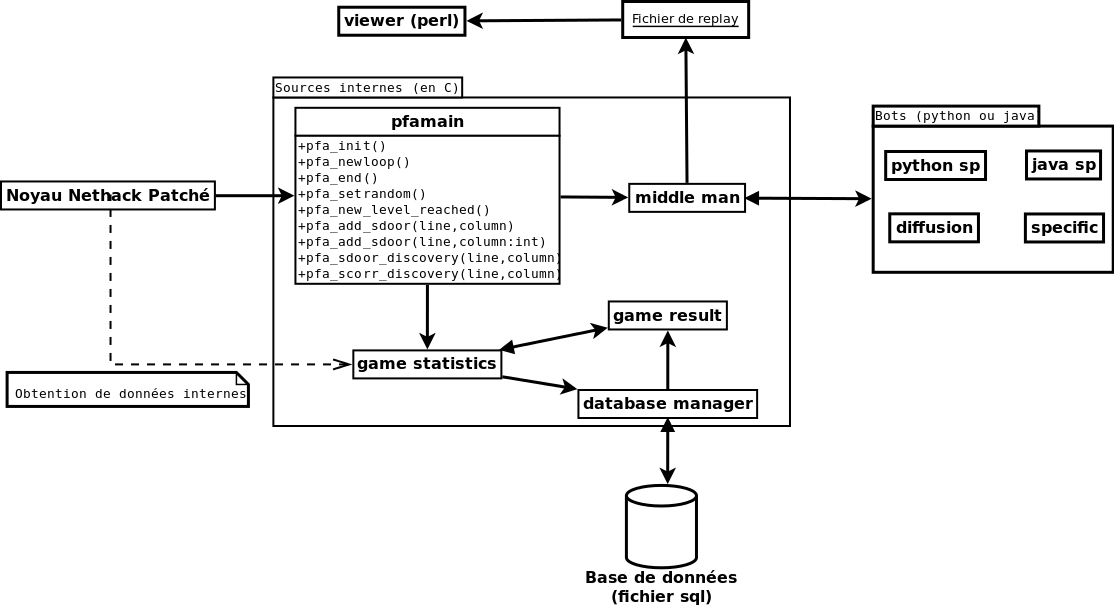
\includegraphics[width=\textwidth]{architecture-finale.png}}
	\caption{\label{fig:architecture} Diagramme de l'architecture finale.}
\end{figure}

\paragraph{Communication avec les bots :}
Les échanges entre les bots et le middle-man sont effectués à l'aide d'une
socket unix, le protocole utilisé entre eux est détaillé dans ce rapport et doit
pouvoir permettre des créer des bots dans d'autres langages.


\paragraph{Patchs :}
L'utilisation des patchs permet de visualiser facilement quels sont les
modifications apportées à nethack. Pour une plus grande facilité de
développement, mais aussi pour plus de clarté, nous avons utilisé autant que
possibles des 'hooks', ceux-ci passant tous par pfamain afin de réduire au
maximum le nombre d'include ajoutés dans les patchs.

\paragraph{Obtention de données par game statistics :}
Afin d'obtenir les données internes au jeu, game statistics doit nécessairement
se servir d'une part du code existant de nethack, afin de connaître le nombre de
cases explorables par exemple.

\paragraph{Gestion de la base de données :}
Les modules {\verb|game_result|} et {\verb|database_manager|} sont étroitement
liés, car tous deux se basent sur la description des différentes tables pour
générer leur code.

\paragraph{Fichier de replay :}
Afin de pouvoir revoir une partie qui s'est jouée, le middle-man fournit une
option permettant de sauvegarder les données envoyées au bot. Celles-ci
peuvent aussi être utilisées pour revoir une partie ou créer une
visualisation de l'exploration à l'aide du programme {\verb|toTikz.pl|}.

\paragraph{Scripts :}
Même s'ils ne sont pas présentés sur ce schéma car ils ne font pas partie
intégrante du logiciel, des scripts bash permettent de créer des graphiques à
partir de base de données qui ont été alimentées par cette version de nethack.


\section{Environnement de création de bots}

\subsection{Prototypage}

NetHack propose, dès sa première version, une interface ASCII qui représente
un donjon sous la forme suivante:

\begin{figure}[H]
\begin{verbatim}
                                           Weapons
                                           a - a blessed +1 mace (weapon in hand)
                                           Armor
   -------        ------------             b - a +0 robe (being worn)
   .......         ........>.|             c - a +0 small shield (being worn)
   |.....|        |..........|             Comestibles
   |......#       |@.........|             e - a clove of garlic
   |<....|#       |..........+             f - a sprig of wolfsbane
   |.....|#       -.---- -----             Spellbooks
   -------############                     g - a spellbook of create monster
         #############                     h - a spellbook of detect food
         # #        ##                     Potions
                                           d - 4 potions of holy water
                      .                    Tools
                      ..                   i - an oil lamp
                       ..                  (end) 
                       ...
                       ...
                       ----

JohnDoe the Aspirant          St:11 Dx:14 Co:13 In:11 Wi:15 Ch:11  Chaotic
Dlvl:1  $:0  HP:14(14) Pw:8(8) AC:7  Exp:1
\end{verbatim}
\end{figure}

Le \verb!@! désigne le joueur, les caractères \verb!|! et \verb!-! sont des
murs, les \verb!#! des couloirs, un \verb!+! symbolise une porte, etc.


\subsubsection*{Séquences d'échappement ANSI}

Cette interface fonctionne à l'aide de caractères d'échappement normalisés
\footnote{http://www.inwap.com/pdp10/ansicode.txt} permettant de contrôler la
position du curseur dans un terminal et d'afficher des caractères à l'endroit
souhaité. Par exemple, une séquence '\verb![46;50H|...+#!' affichera la chaîne
de caractères '\verb!|...+#!' en commençant à la ligne 46, colonne 50. Il est
alors facile de reconstituer une carte envoyée par le jeu: le '\verb!|!' est
aux coordonnées (46, 50), le '\verb!+!' est situé à (46, 54), etc.
	
Le projet TAEB (Tactical Amulet Extraction Bot)
\footnote{https://github.com/sartak/TAEB} utilise ce principe pour
reconstituer la carte à l'aide d'un module sachant interpréter ces séquences
de caractères \footnote{https://metacpan.org/module/Term::VT102}. Une première
approche fut donc de copier ce procédé.


\subsubsection*{Pseudo-terminal}

Pour s'assurer de la disponibilité de certaines fonctionnalités lorsqu'il est
utilisé avec son interface ASCII, NetHack procède à quelques vérifications
pour s'assurer qu'il est bien lancé depuis un terminal. Cela empêche les
redirections de son entrée/sortie car il refuse alors de s'exécuter. Les
quelques lignes de code responsables peuvent être désactivées sans conséquence
notable sur le reste du jeu mais cela nécessite de modifier le code original.
Pour rediriger à la fois l'entrée et la sortie du jeu sans modifier le jeu, il
est nécessaire de 'tromper' NetHack à l'aide d'un pseudo terminal.

Un pseudo terminal (pty) est une paire de pseudo périphériques dont l'un est
appelé 'maître' et l'autre 'esclave'. Le maître est utilisé comme un terminal
standard sur lequel on peut écrire ou lire du texte. L'esclave communique avec
l'application et sert simplement de rapporteur entre la partie 'maître' et
NetHack. Ainsi, le jeu est satisfait puisqu'il est lancé depuis un terminal et
il peut maintenant être contrôlé depuis la partie 'master' du pty sur laquelle
on souhaite brancher un bot \footnote{Plus de détails avec la page de manuel
pty(7)}.


\subsubsection*{Décomposition de l'affichage}

Lorsqu'il est lancé depuis un terminal, l'interface ASCII détecte le nombre de
lignes et de colonnes disponibles afin de faire des défilements ou des
superpositions de menus lorsque nécessaire \footnote{voir libtermcap}. Cela
pose problème avec la méthode consistant à interpréter les séquences
d'échappement car il faut être capable détecter lorsque deux éléments se
chevauchent.

\begin{figure}[h]
	\caption{Exemple d'un menu recouvrant une partie de la carte}
	\begin{verbatim}
                                     Weapons
                                     a - a blessed +1 mace (weapon in hand)
             ------                  i - a crude bow
             |...[|                  Armor
 -------     |..<..###############`  b - a +0 robe (being worn)
 |......-    .....|       ---------- c - a +0 small shield (being worn)
 |           -.----      #.........| Comestibles
              ##       ###|........| e - a clove of garlic
               #       #  |........| f - a sprig of wolfsbane
               ###   ###  |........| Spellbooks
                 #   #    |........| g - a spellbook of detect food
                 ### #    |........| h - a spellbook of clairvoyance
                ?  # #    --.------- Potions
               ----.-#      ###@#### d - 4 potions of holy water
               |....|#               j - a blessed black potion
               |....|#               (end) 
               +.....#                         |..... ..$|
               |....|                          |.........|
               ------                          |.........|
                                               -----------

JohnDoe the Aspirant          St:10 Dx:14 Co:13 In:9 Wi:18 Ch:11  Chaotic
Dlvl:1  $:0  HP:14(14) Pw:7(7) AC:7  Exp:1
	\end{verbatim}
\end{figure}

Une façon de supprimer cette difficulté est de tromper une nouvelle fois
NetHack en manipulant la taille effective du pseudo terminal qui n'est en rien
liée à sa taille réelle à l'écran. Avec une taille assez grande, il n'y a
jamais de chevauchement.

Nous pouvons ainsi séparer l'écran comme suit en forçant une taille de 24
lignes par 160 colonnes :

\begin{figure}[H]
\begin{verbatim}
               Messages line ................ --more--
               ----------------------------------------
               |                  |                   |
               |                  |                   |
               |    MAP 21x80     |     MENU 21x80    |
               |                  |                   |
               |                  |                   |
               ----------------------------------------
               Status line 1 .........................
               Status line 2 .........................
\end{verbatim}
\end{figure}

\subsubsection*{Branchement d'un bot}

Cette interface permettait à un bot de communiquer avec NetHack depuis une
machine distante (UDP ou TCP interchangeables) sans aucune modification du jeu
original. Dans la version présentée dans le premier livrable, l'intégralité de
la carte était retransmise au bot et les échanges avec le jeu souffraient de
l'overhead des packets TCP ou UDP lorsque le bot et NetHack tournaient sur la
même machine. Des améliorations alors envisagées étaient d'établir un
protocole de communication plus complexe pour n'envoyer que les éléments ayant
changé et de recourir aux sockets Unix pour des communications locales.

Les communications entre l'interface et un bot utilisaient le protocole
suivant.

\paragraph{interface vers bot:} À chaque tour, l'information envoyée par
l'interface commence par \verb!START! et se termine par \verb!END!. Pour
toutes les différentes transmissions, il existe deux possibilités différentes
:
\begin{itemize}
	\item Mono-ligne \verb!<NOM_VARIABLE> <VARIABLE_1> <VARIABLE_2> ...!
	\item Multi-ligne
		\begin{verbatim}
		START <NOM_VARIABLE>
		...
		...
		END <NOM_VARIABLE>
		\end{verbatim}
\end{itemize}
Les caractères représentant la carte sont transmis sans transformation. Exemple:
\begin{figure}[H]
\begin{verbatim}
START
DUNGEON_LEVEL 1
MAP_HEIGHT 6
MAP_WIDTH 10
START MAP
          
   ----   
  |...@+  
  |....|  
   ----   
          
END MAP
END
\end{verbatim}
\end{figure}

\paragraph{bot vers interface:} À chaque tour le bot peut accomplir une et une
seule action. Une action est définie par son type et ses paramètres (ex :
l'action d'attaquer est définie par son type 'attaque' et la direction de
l'attaque). Les actions possibles étaient définies par un langage faisant
abstraction des commandes au clavier de NetHack :
\begin{itemize}
	\item Déplacement : \verb!MOVE <direction>!
	\item Ouvrir porte : \verb!OPEN <direction>!
	\item Lancer une recherche : \verb!SEARCH!
	\item Forcer une porte : \verb!FORCE <direction>! (permet d'ouvrir les portes verrouillées)
\end{itemize}
\noindent La direction étant un élément parmi \verb!NORTH!, \verb!SOUTH!,
\verb!WEST!, \verb!EAST!, \verb!NORTH_WEST!, \verb!NORTH_EAST!,
\verb!SOUTH_WEST!, \verb!SOUTH_EAST!, \verb!UP!, \verb!DOWN!.


\subsection{Modifications de NetHack}

\subsubsection{Interface finale}

\paragraph{}À la demande du client et du responsable pédagogique,
l'utilisation d'une interface intégrée directement dans le jeu fut
implémentée. Elle permet d'économiser une étape d'entrée/sortie lors de la
communication avec un bot mais a le désavantage de rendre impossible
l'utilisation du projet sur une version originale du jeu.


Pour cela, nous avons utilisé une structure fournie par le NetHack regroupant
des pointeurs de fonction à appeler lors d'un évènement à communiquer au
joueur. C'est sur ce mécanisme que repose la plupart des interfaces graphiques
existantes pour le jeu. Les principales fonctions appelées sont les suivantes
:
\begin{itemize}
	\item \verb!int *_create_nhwindows(type)! : cette fonction est appelée
		lors de la création d'une fenêtre (afficher un menu par exemple). Le
		type donné en paramètre donne la nature de la fenêtre et sa valeur
		peut être \verb!NHW_MAP!, \verb!NHW_SATUS!, \verb!NHW_MESSAGE!,
		\verb!NHW_MENU!, \verb!NHW_TEXT!. En comparaison avec le découpage de
		l'écran de l'interface précédente, cette façon de distinguer les
		différentes fenêtres est beaucoup moins sujette à erreur et ne devrait
		pas souffrir d'un changement d'organisation des fenêtres si un jour
		NetHack devait évoluer.
	\item \verb!void *_clear_nhwindow(id)! : cette fonction ne fait qu'effacer
		le contenu d'une fenêtre mais elle est intéressante dans le cas où
		\verb!id! est l'identifiant de la fenêtre associée à la carte. En
		effet, c'est un moyen simple, bien que peu sûr, de détecter un
		changement d'étage au niveau de l'interface. La détection certaine
		d'un changement d'étage peut néanmoins se faire au niveau du client
		(le bot) qui comprendra qu'un effacement de la carte juste après une
		montée ou une descente d'une échelle correspond effectivement à un
		changement d'étage.
	\item \verb!void *_print_glyph(id, x, y, glyph)! : cette fonction sert à
		communiquer au joueur qu'un glyph dans la fenêtre d'identifiant
		\verb!id! se situe aux coordonnées \verb!(x, y)!. \verb!glyph! est un
		entier unique à chaque élément du jeu. NetHack fourni une fonction
		\verb!map_glyph! qui le transforme en un caractère qui peut être
		directement affiché à l'écran (\verb!@! pour un joueur, \verb!+! pour
		une porte, etc.). Cette dernière fonction peut retourner des
		caractères identiques pour des glyphs différents et cela est à prendre
		en compte lors de l'élaboration du protocole pour éviter des
		confusions au niveau du bot.
	\item \verb!char *_yn_function(query,resp, def)! : cette fonction est
		appelée dès lors que NetHack pose une question au client. Le nom est
		trompeur car elle ne sert pas seulement aux questions dont la réponse
		est 'yes' ou 'no'. Elle est utilisée par exemple pour savoir dans
		quelle direction frapper si le client donne l'ordre de combattre.
	\item \verb!int *_nh_poskey(x, y, mod)! : cette fonction attend une
		commande de l'utilisateur. Les paramètres ne nous concernent pas car
		ils sont utilisés dans le cas où l'interface supporte la souris.
\end{itemize}

\paragraph{}Le paramétrage se fait avec des variables d'environnement :
\begin{itemize}
\item \verb!NH_MM_SOCKPATH! : spécifier un chemin pour la socket unix
	(permettant la communication entre NetHack et les bots) à créer. Par
	défaut, le middleman créé {\verb|/tmp/mmsock|}.
\item \verb!NH_MM_DUPMSGS! : si mise à une valeur différente de 0, cette
	variable active l'enregistrement de la partie dans le fichier
	{\verb|nethackdir/replay|}. Désactivée par défaut.
\item \verb!NH_MM_LOGGING! : si mise à une valeur différente de 0, cette
	variable active l'enregistrement de logs du middleman dans le fichier
	{\verb|nethackdir/mm.log|}. Désactivée par défaut.
\item \verb!NH_MM_TIMEOUT! : spécifie le timeout en secondes pour les
	communications avec le bot. Si le bot met un temps en secondes supérieur à
	cette valeur, le middleman quitte la partie. Par défaut, cette variables
	est mise à 2 secondes.
\item \verb!NH_MAX_MOVES! :
  Ce paramètre spécifie le nombre de mouvement maximal autorisé au bot, sachant
  que le bot n'est pas sensé mourir, c'est la définition de ce paramètre qui
  spécifiera la durée de la partie. Par défaut, cette variable vaut 20000.
\item \verb!NH_DATABASE_PATH! :
  Spécifie le chemin d'accès pour la base de données à laquelle les résultats
  seront ajoutés. Par défaut, ce chemin vaut {\verb|/tmp/test.db|}.
\item \verb!NH_BOT_NAME! :
  Permet d'indiquer le nom du bot afin d'ajouter une entrée complète à la base
  de données. Par défaut : la valeur est \emph{unknown}.
\item \verb!NH_MODE_NAME! :
  Permet d'indiquer le nom du mode utilisé afin de l'ajouter correctement à la
  base de données. Par défaut : la valeur est {\verb|seek_secret|}.
\item \verb!NH_SEED! :
  Permet de donner la valeur de la graine à utiliser pour l'initialisation du
  générateur de nombres aléatoires de NetHack. Par défaut, si cette
  valeur n'est pas spécifiée, la graine utilisée est une combinaison du nombre
  de secondes et de millisecondes écoulées depuis l'epoch \footnote{$1^{er}$
  janvier 1970 à 0 heure (UTC)}.

\end{itemize}

\paragraph{} Cette nouvelle interface ne permet plus d'observer, depuis
NetHack, le comportement du bot. Le jeu propose diverses interfaces
graphiques, une solution aurait donc très bien pu être de rediriger les appels
aux fonctions de l'interface que nous avons développée vers celles d'une
interface existante. Cependant, cela pose un problème non négligeable : les
différentes interfaces graphiques s'autorisent des fonctions bloquantes
(fenêtre de dialogue propres à chacune d'elles par exemple). A moins de
supprimer ou d'adapter les fonctions gênantes pour chacune d'elles, il n'est
pas envisageable d'utiliser cette solution avec un bot.

Une autre solution aurait été de permettre un affichage simple dans le
terminal. Cela n'a pas été retenu car cela aurait consisté à faire des
traitements supplémentaires pour reconstituer la carte et cela reviendrait à
dupliquer le travail que le bot doit déjà faire de lui même.

\paragraph{} Le protocole de communication entre un bot et le jeu a été
modifié depuis le prototype. L'interface retransmet à l'identique au noyau de
NetHack les commandes transmises par le bot. C'est à dire que le client doit
utiliser les commandes originales du jeu et que le langage faisant abstraction
de celles-ci a été abandonné. Exception est faite des commandes commençant par
'\verb!#!' qui ne sont pas supportées. Ceci est dû au code original de NetHack
qui cherche à réaliser des traitements particuliers pour ce type de commande
(auto complétion, etc.) que nous n'avons pas jugé utile d'implémenter.

Un bot peut envoyer plusieurs commandes à la fois ce qui peut se montrer utile
pour diminuer le nombre d'échanges avec le jeu et ou d'appels systèmes pour un
gain de performances. Les commandes à envoyer en une seule fois est toutefois
limitée à 64 octets. Par exemple, envoyer les commandes '\verb!jjkl!' aura le
même effet que d'envoyer chacune des lettres séparément et fera bouger le
joueur deux fois vers le bas, une fois vers le haut et une fois vers la
droite. Il est donc recommandé au développeur d'un bot de prendre en charge
des patterns : '\verb!oj!' pour ouvrir une porte au sud, etc.

Quant au protocole concernant les échanges depuis l'interface vers le bot,
nous avons établi les règles suivantes :
\begin{itemize}
	\item \verb!S! marque le début d'une transmission
	\item \verb!E! marque la fin d'une transmission et indique que l'interface
		attend une commande du client.
	\item \verb!g<x><y><glyph><code>! indique qu'un élément du jeu représenté
		par le caractère \verb!glyph! et ayant pour code identificateur
		\verb!code! \footnote{Voir annexe pour les différents codes
		importants} se trouve aux coordonnées \verb!(x, y)!.
	\item \verb!C! indique que la carte doit être effacée. Un bot peut
		interpréter cette information comme étant un changement d'étage réussi
		s'il venait d'envoyer une commande descente ou montée d'escalier.
\end{itemize}


\subsubsection{Développement par les patchs}

\paragraph{} L'un de nos objectifs était d'adapter NetHack en ayant la plus
petite empreinte possible sur le code existant. C'est dans ce but que nous
avons opté pour l'installation de 'hooks' dans le code source faisant appels à
nos fonctions définies dans leur propre emplacement, dans un répertoire
séparé. Ces points d'entrés sont placés à des endroits stratégiques :
\begin{itemize}
	\item Le premier est installé dans la fonction \verb!moveloop()! de
		\verb!allmain.c! du jeu qui est exécutée par toutes les architectures
		supportées. Elle fait alors appel à \verb!pfa_init()! du fichier
		\verb!pfamain.c! et se situe juste avant la boucle principale.
		\verb!pfa_init()! regroupe toutes les procédures d'initialisation
		nécessaires au modules que nous avons développés.
	\item Le second se trouve au début la boucle principale de
		\verb!moveloop()! pour nous permettre d'effectuer des traitements à
		chaque tour de jeu. Il fait appel à \verb!pfa_newloop()!.
	\item Le dernier est placé dans la fonction \verb!terminate(status)! du
		fichier \verb!end.c! appelée lorsque NetHack quitte afin de nous
		donner l'occasion de terminer proprement (libération de la mémoire,
		fermeture des fichiers, etc.). Il fait appel à \verb!pfa_end()!.
\end{itemize}

\paragraph{} Nous souhaitions également pouvoir livrer nos modifications
indépendamment du jeu lui même. Nous avons donc utilisé un système de patchs
installant les points d'entrée aux endroits voulus. Ce même procédé est
utilisé pour les modifications correspondant aux 'modes' (suppression des
monstres, suppression des objets, etc.). Le processus d'installation a été
automatisé pour qu'à partir d'une archive originale de NetHack le code source
soit patché pour prendre en compte nos ajouts et modifications.

\paragraph{} 
\textbf{TODO David: configuration des patchs à appliquer pour chaque mode et
	expliquer ce que ces patchs font + donner un exemple de patch avec détail
	des lignes changées et l'effet sur le jeu.}
Nous avons définis deux catégories de patchs : nécessaires ou facultatifs.
Des patchs sont nécessaires lorsqu'ils permettent le fonctionnement des
modules que nous avons ajoutés (ce sont notamment les patchs ajoutant des
points d'entrée). Les patchs facultatifs sont majoritairement ceux qui
définissent les modes de jeu or il est tout à fait possible de faire jouer les
bots sur une version de nethack dans laquelle aucun danger n'est désactivé,
ces derniers mourront plus rapidement.

Les patchs nécessaires sont automatiquement appliqués au code de NetHack lors
de la compilation du projet et sont regroupés dans le dossier \verb!install/!.
Si de nouveaux modules devaient être ajoutés au projet, il faudrait donc créer
les patchs correspondant (la création d'un patch est expliquée plus loin) et
les placer dans le dossier \verb!install!. Le nom de ces patchs doit être de
la forme \verb!<nom_du_patch>.patch! afin d'être automatiquement détectés par
le script d'installation \verb!nh-setup.sh!. 

\paragraph{Création de patchs :}

\subsection{Développement de bots.}

\subsubsection{'Bot' contrôlé à la main}

L'interface développée ne permet plus de jouer au jeu à la main et donc de
tester nous même les modifications apportées au jeu. Nous avons donc développé
un client adapté au protocole mis en place. Il s'agit du programme
\verb!bots/dummy-client.pl!. Il accepte les mêmes commandes que le jeu original et
nous a permis, entre autre, de tester l'effet des patchs sur une partie.


\subsubsection{Le starter package java}
Afin de pouvoir rapidement commencer à coder des bots, un \emph{starter package}
en java est fourni, les fonctionnalités fournies sont principalement la lecture
de la carte et la vérification de la validité des mouvements.
\\
Ce bot se contente de lister les actions possibles et d'en choisir une de façon
aléatoire, avec tout de même certaines actions prioritaires. Cette base permet
de pouvoir tester différentes stratégie sans avoir à implémenter à nouveau la
réception et l'envoi de message aux bots.

\subsubsection{Le bot diffusion}
Le principe de ce bot est d'établir des scores pour chaque cases et de diffuser
ensuite les valeurs à tous les voisins, ainsi la principale différence avec les
autres bots est que la complexité est bien plus élevée étant donnée que pour
choisir la prochaine action, il n'y a pas que le voisinage immédiat qui est
observé. Ce surcoût de temps permet en revanche d'avoir des meilleurs résultats
et la possibilité de modifier les scores facilement permet de changer les
objectifs en changeant uniquement des constantes.
\\
Une fois tous les scores calculés et la diffusion effectuée, l'action choisie
est celle ayant le score le plus élevé parmi celles qui sont autorisées. Ce bot
est donc totalement déterministe. Quelques attentions ont été portées à
l'optimisation afin de réduire légèrement le temps d'exécution, cependant, il
est certainement possible d'améliorer encore grandement les performances en
optimisant certaines parties du code.

\subsubsection{Le starter package python}

Ce bot propose un squelette pour l'interprétation des messages venant du jeu
et un algorithme simple pour l'exploration 'rapide' d'un niveau en maintenant
un compteur pour chaque case visitée. Le bot se déplace en priorité sur les
cases les moins visitées.

\subsubsection{Le bot spécialisé}

Ce bot, écrit en python, n'a pas vocation à être utilisé dans des conditions
"normales" de jeu. C'est un bot dédié à la résolution optimale d'un problème
particulier : trouver, en un nombre de tours minimal, la porte secrète cachée
de façon aléatoire dans une salle carrée de taille 10x10. Une étude théorique
de ce problème a été réalisée et ce bot a pour but de s'approcher de la
solution optimale. Ceci permet d'effectuer une comparaison avec les autres
bots qui sont plus "généralistes".

Afin d'utiliser ce bot dans les bonnes conditions, il est nécessaire d'avoir
compilé une version du jeu dans laquelle le patch
{\verb|patches/create_level.patch|} a été appliqué. Ce patch modifie le donjon
de telle sorte que le premier niveau ne contienne qu'une seule salle de la
forme décrite précédemment (ce niveau ne contient pas d'escalier pour
descendre dans les niveaux suivants).

\subsubsection{Ajouter un bot}

Plusieurs facilités ont été offertes pour de futurs ajouts de bots. La
première est la possibilité d'intégrer automatiquement la compilation de ce
nouveau bots à celle des autres. En effet, un \verb!Makefile! se trouve dans le
dossier \verb!bots/! et permet de compiler l'ensemble des bots pour lesquels
cela est nécessaire (par exemple les bots écris en Java). Lorsque la
commande \verb!make! est exécutée depuis dossier, l'ensemble des sous dossiers
est exploré automatiquement afin de repérer ceux possédant un fichier nommé
\verb!Makefile!. Dans chacun de ces dossiers (correspondant à un bot
particulier) est exécutée la commande \verb!make! afin de compiler les sources
du bot en question.

Ainsi, lors de la création d'un nouveau bot, il suffit de créer un dossier
dédié à ce bot dans \verb!bots/! et d'écrire le fichier \verb!Makefile! qui
permet de compiler ses sources, si besoin\footnote{Un bot écrit dans un
langage interprété tel que Python n'aura pas besoin du \verb!Makefile!.}.

TODO David : décrire le fichier bots.conf

\subsection{Outils d'analyse et de deboguage}

Plusieurs outils ont été mis à disposition pour faciliter le développement des
bots et l'analyse de leurs performances.

\subsubsection{Rejouer une partie}

\textbf{TODO: David} Parler de l'extraction de la graine.

\subsubsection{Voir ou revoir une partie}

\paragraph{}
En mettant la variable d'environnement \verb!NH_MM_DUPMSGS! à une valeur
différente de 0 lors du lancement du jeu, le middleman dupliquera tous les
messages envoyées au bot vers la sortie standard. Cette sortie peut être
redirigée vers le programme \verb!bots/dummy-client.pl! qui s'exécutera alors en
'lecture seule' \footnote{\verb!bots/dummy-client.pl! a plusieurs modes
d'exécution} et interprétera le flux pour afficher la carte correspondante à
la partie en cours.

En redirigeant cette sortie vers un fichier (ou en lançant le script
\verb!game_runner.sh! avec l'option \verb!-r!), le déroulement de la partie
peut être sauvegardée.  Le programme \verb!viewer/viewer.pl! permet
d'exploiter cette sauvegarde afin de visualiser la partie a posteriori. Ses fonctionnalités sont :
\begin{itemize}
	\item reconstitution tour par tour
	\item revenir en arrière tour par tour
	\item saut direct à un numéro de tour donné
	\item 'diaporama' par incrémentation ou décrémentation d'un nombre de
		tours par seconde donné
\end{itemize}

\paragraph{}
Un échange entre l'interface et le bot au tour $N$ ne permet pas de
reconstituer l'état de la partie au tour $N$ car seules les mises à jour sont
transmises. Il est donc nécessaire de traiter tous les échanges depuis le
début de la partie pour connaître l'état du jeu à un tour donné. La
reconstitution de longues parties peut alors devenir lente pour des opérations
simples. Par exemple, passer du tour 2000 au tour 1999 nécessiterait de
rejouer 1999 tours pour faire un simple saut en arrière.

Une meilleure exploitation des informations contenues dans le fichier de
replay est de calculer l'inverse des mises à jour qu'il contient et/ou de
stocker des états paliers du jeu (tous les 100 tours par exemple). Dans
\verb!viewer.pl! seule la méthode des mises à jour inverses est implémentée.
Elles permettent de revenir en arrière rapidement et un passage d'un tour $N$
à un tour $M$ se fait simplement en traitant tous les tours de $N$ à $M$ si
$|N-M| < M$ ou de $0$ à $M$ sinon. Certains paliers sont tout de même utilisés
lors du changement de niveaux pour ne pas avoir à retracer les salles des
niveaux inférieurs qui seront de toute manière effacées lors d'un retour en
arrière.

\subsubsection{Aperçu du nombre de visites sur chaque case}

\paragraph{}
Une sauvegarde peut également être utilisé dans d'autres buts.
Par exemple, un simple programme comptant le nombre de visite sur chaque
coordonnée permet de produire les images suivantes à l'aide de TikZ :

\begin{figure}[H]
	\caption{Nombre de visites sur chaque case sur deux niveaux du starter
	package java. En blanc les cases non visitées, en jaune clair les cases
visitées peu de fois, en rouge les cases visitées un grand nombre de fois.}
	\resizebox{\columnwidth}{!}{\begin{tikzpicture}[scale=0.3]
\node at (2, -27) {\verb!-!};
\node at (3, -27) {\verb!-!};
\node at (4, -27) {\verb!-!};
\node at (5, -27) {\verb!-!};
\node at (6, -27) {\verb!-!};
\node at (7, -27) {\verb!-!};
\node at (8, -27) {\verb!-!};
\node at (9, -27) {\verb!-!};
\node at (10, -27) {\verb!-!};
\node at (11, -27) {\verb!-!};
\node at (21, -27) {\verb!-!};
\node at (22, -27) {\verb!-!};
\node at (23, -27) {\verb!-!};
\node at (24, -27) {\verb!-!};
\node at (25, -27) {\verb!-!};
\node at (26, -27) {\verb!-!};
\node at (27, -27) {\verb!-!};
\node at (28, -27) {\verb!-!};
\node at (29, -27) {\verb!-!};
\node at (30, -27) {\verb!-!};
\node at (31, -27) {\verb!-!};
\node at (32, -27) {\verb!-!};
\node at (33, -27) {\verb!-!};
\node at (34, -27) {\verb!-!};
\node at (35, -27) {\verb!-!};
\node at (2, -28) {\verb!|!};
\node [fill=red!44!yellow] at (3, -28) {\verb!.!};
\node [fill=red!57!yellow] at (4, -28) {\verb!.!};
\node [fill=red!51!yellow] at (5, -28) {\verb!.!};
\node [fill=red!53!yellow] at (6, -28) {\verb!.!};
\node [fill=red!56!yellow] at (7, -28) {\verb!.!};
\node [fill=red!57!yellow] at (8, -28) {\verb!.!};
\node [fill=red!49!yellow] at (9, -28) {\verb!.!};
\node [fill=red!33!yellow] at (10, -28) {\verb!.!};
\node at (11, -28) {\verb!|!};
\node at (21, -28) {\verb!|!};
\node [fill=red!11!yellow] at (22, -28) {\verb!.!};
\node [fill=red!11!yellow] at (23, -28) {\verb!.!};
\node [fill=red!13!yellow] at (24, -28) {\verb!.!};
\node [fill=red!7!yellow] at (25, -28) {\verb!.!};
\node [fill=red!6!yellow] at (26, -28) {\verb!.!};
\node [fill=red!6!yellow] at (27, -28) {\verb!.!};
\node [fill=red!6!yellow] at (28, -28) {\verb!.!};
\node [fill=red!4!yellow] at (29, -28) {\verb!.!};
\node [fill=red!3!yellow] at (30, -28) {\verb!.!};
\node [fill=red!9!yellow] at (31, -28) {\verb!.!};
\node [fill=red!6!yellow] at (32, -28) {\verb!.!};
\node [fill=red!4!yellow] at (33, -28) {\verb!.!};
\node [fill=red!3!yellow] at (34, -28) {\verb!.!};
\node at (35, -28) {\verb!|!};
\node at (2, -29) {\verb!|!};
\node [fill=red!68!yellow] at (3, -29) {\verb!.!};
\node [fill=red!79!yellow] at (4, -29) {\verb!.!};
\node [fill=red!95!yellow] at (5, -29) {\verb!.!};
\node [fill=red!97!yellow] at (6, -29) {\verb!.!};
\node [fill=red!83!yellow] at (7, -29) {\verb!.!};
\node [fill=red!100!yellow] at (8, -29) {\verb!.!};
\node [fill=red!69!yellow] at (9, -29) {\verb!.!};
\node [fill=red!59!yellow] at (10, -29) {\verb!.!};
\node [fill=red!36!yellow] at (11, -29) {\verb!.!};
\node [fill=red!16!yellow] at (12, -29) {\verb!#!};
\node [fill=red!15!yellow] at (13, -29) {\verb!#!};
\node [fill=red!13!yellow] at (14, -29) {\verb!#!};
\node at (21, -29) {\verb!|!};
\node [fill=red!16!yellow] at (22, -29) {\verb!.!};
\node [fill=red!20!yellow] at (23, -29) {\verb!.!};
\node [fill=red!14!yellow] at (24, -29) {\verb!.!};
\node [fill=red!16!yellow] at (25, -29) {\verb!.!};
\node [fill=red!12!yellow] at (26, -29) {\verb!.!};
\node [fill=red!10!yellow] at (27, -29) {\verb!.!};
\node [fill=red!6!yellow] at (28, -29) {\verb!.!};
\node [fill=red!6!yellow] at (29, -29) {\verb!.!};
\node [fill=red!8!yellow] at (30, -29) {\verb!.!};
\node [fill=red!8!yellow] at (31, -29) {\verb!.!};
\node [fill=red!10!yellow] at (32, -29) {\verb!.!};
\node [fill=red!8!yellow] at (33, -29) {\verb!.!};
\node [fill=red!6!yellow] at (34, -29) {\verb!.!};
\node at (35, -29) {\verb!|!};
\node at (2, -30) {\verb!|!};
\node [fill=red!60!yellow] at (3, -30) {\verb!.!};
\node [fill=red!94!yellow] at (4, -30) {\verb!.!};
\node [fill=red!75!yellow] at (5, -30) {\verb!.!};
\node [fill=red!86!yellow] at (6, -30) {\verb!.!};
\node [fill=red!89!yellow] at (7, -30) {\verb!.!};
\node [fill=red!92!yellow] at (8, -30) {\verb!.!};
\node [fill=red!89!yellow] at (9, -30) {\verb!.!};
\node [fill=red!58!yellow] at (10, -30) {\verb!.!};
\node at (11, -30) {\verb!|!};
\node [fill=red!25!yellow] at (14, -30) {\verb!#!};
\node [fill=red!16!yellow] at (20, -30) {\verb!#!};
\node [fill=red!22!yellow] at (21, -30) {\verb!.!};
\node [fill=red!19!yellow] at (22, -30) {\verb!.!};
\node [fill=red!16!yellow] at (23, -30) {\verb!.!};
\node [fill=red!20!yellow] at (24, -30) {\verb!.!};
\node [fill=red!13!yellow] at (25, -30) {\verb!.!};
\node [fill=red!10!yellow] at (26, -30) {\verb!.!};
\node [fill=red!10!yellow] at (27, -30) {\verb!.!};
\node [fill=red!8!yellow] at (28, -30) {\verb!.!};
\node [fill=red!8!yellow] at (29, -30) {\verb!.!};
\node [fill=red!5!yellow] at (30, -30) {\verb!.!};
\node [fill=red!8!yellow] at (31, -30) {\verb!.!};
\node [fill=red!6!yellow] at (32, -30) {\verb!.!};
\node [fill=red!13!yellow] at (33, -30) {\verb!.!};
\node [fill=red!7!yellow] at (34, -30) {\verb!.!};
\node at (35, -30) {\verb!|!};
\node at (41, -30) {\verb!-!};
\node at (42, -30) {\verb!-!};
\node at (43, -30) {\verb!-!};
\node at (44, -30) {\verb!-!};
\node at (45, -30) {\verb!-!};
\node at (2, -31) {\verb!|!};
\node [fill=red!43!yellow] at (3, -31) {\verb!.!};
\node [fill=red!63!yellow] at (4, -31) {\verb!.!};
\node [fill=red!63!yellow] at (5, -31) {\verb!.!};
\node [fill=red!54!yellow] at (6, -31) {\verb!.!};
\node [fill=red!58!yellow] at (7, -31) {\verb!.!};
\node [fill=red!62!yellow] at (8, -31) {\verb!.!};
\node [fill=red!51!yellow] at (9, -31) {\verb!.!};
\node [fill=red!29!yellow] at (10, -31) {\verb!.!};
\node at (11, -31) {\verb!|!};
\node [fill=red!18!yellow] at (14, -31) {\verb!#!};
\node [fill=red!29!yellow] at (15, -31) {\verb!#!};
\node [fill=red!18!yellow] at (16, -31) {\verb!#!};
\node [fill=red!13!yellow] at (18, -31) {\verb!#!};
\node [fill=red!27!yellow] at (19, -31) {\verb!#!};
\node [fill=red!20!yellow] at (20, -31) {\verb!#!};
\node at (21, -31) {\verb!|!};
\node [fill=red!18!yellow] at (22, -31) {\verb!.!};
\node [fill=red!20!yellow] at (23, -31) {\verb!.!};
\node [fill=red!18!yellow] at (24, -31) {\verb!.!};
\node [fill=red!9!yellow] at (25, -31) {\verb!.!};
\node [fill=red!4!yellow] at (26, -31) {\verb!.!};
\node [fill=red!4!yellow] at (27, -31) {\verb!.!};
\node [fill=red!6!yellow] at (28, -31) {\verb!.!};
\node [fill=red!4!yellow] at (29, -31) {\verb!.!};
\node [fill=red!3!yellow] at (30, -31) {\verb!.!};
\node [fill=red!2!yellow] at (31, -31) {\verb!.!};
\node [fill=red!9!yellow] at (32, -31) {\verb!.!};
\node [fill=red!6!yellow] at (33, -31) {\verb!.!};
\node [fill=red!4!yellow] at (34, -31) {\verb!.!};
\node at (35, -31) {\verb!|!};
\node at (41, -31) {\verb!|!};
\node [fill=red!7!yellow] at (42, -31) {\verb!.!};
\node [fill=red!12!yellow] at (43, -31) {\verb!.!};
\node [fill=red!10!yellow] at (44, -31) {\verb!.!};
\node at (45, -31) {\verb!|!};
\node at (2, -32) {\verb!-!};
\node at (3, -32) {\verb!-!};
\node [fill=red!41!yellow] at (4, -32) {\verb!.!};
\node at (5, -32) {\verb!-!};
\node at (6, -32) {\verb!-!};
\node at (7, -32) {\verb!-!};
\node at (8, -32) {\verb!-!};
\node at (9, -32) {\verb!-!};
\node at (10, -32) {\verb!-!};
\node at (11, -32) {\verb!-!};
\node [fill=red!31!yellow] at (16, -32) {\verb!#!};
\node [fill=red!31!yellow] at (18, -32) {\verb!#!};
\node at (21, -32) {\verb!-!};
\node at (22, -32) {\verb!-!};
\node [fill=red!12!yellow] at (23, -32) {\verb!.!};
\node at (24, -32) {\verb!-!};
\node at (25, -32) {\verb!-!};
\node at (26, -32) {\verb!-!};
\node at (27, -32) {\verb!-!};
\node at (28, -32) {\verb!-!};
\node at (29, -32) {\verb!-!};
\node at (30, -32) {\verb!-!};
\node at (31, -32) {\verb!-!};
\node at (32, -32) {\verb!-!};
\node at (33, -32) {\verb!-!};
\node at (34, -32) {\verb!-!};
\node at (35, -32) {\verb!-!};
\node at (41, -32) {\verb!|!};
\node [fill=red!10!yellow] at (42, -32) {\verb!.!};
\node [fill=red!24!yellow] at (43, -32) {\verb!.!};
\node [fill=red!17!yellow] at (44, -32) {\verb!.!};
\node at (45, -32) {\verb!|!};
\node at (72, -32) {\verb!|!};
\node [fill=red!16!yellow] at (4, -33) {\verb!#!};
\node [fill=red!24!yellow] at (5, -33) {\verb!#!};
\node [fill=red!11!yellow] at (6, -33) {\verb!#!};
\node [fill=red!9!yellow] at (7, -33) {\verb!#!};
\node [fill=red!12!yellow] at (8, -33) {\verb!#!};
\node [fill=red!6!yellow] at (9, -33) {\verb!#!};
\node [fill=red!15!yellow] at (16, -33) {\verb!#!};
\node [fill=red!40!yellow] at (17, -33) {\verb!#!};
\node [fill=red!21!yellow] at (18, -33) {\verb!#!};
\node [fill=red!3!yellow] at (23, -33) {\verb!#!};
\node [fill=red!4!yellow] at (24, -33) {\verb!#!};
\node [fill=red!4!yellow] at (25, -33) {\verb!#!};
\node [fill=red!2!yellow] at (26, -33) {\verb!#!};
\node at (39, -33) {\verb!#!};
\node at (40, -33) {\verb!#!};
\node at (41, -33) {\verb!+!};
\node [fill=red!14!yellow] at (42, -33) {\verb!.!};
\node [fill=red!21!yellow] at (43, -33) {\verb!.!};
\node [fill=red!21!yellow] at (44, -33) {\verb!.!};
\node at (45, -33) {\verb!|!};
\node [fill=red!6!yellow] at (46, -33) {\verb!#!};
\node [fill=red!8!yellow] at (47, -33) {\verb!#!};
\node [fill=red!6!yellow] at (48, -33) {\verb!#!};
\node [fill=red!1!yellow] at (49, -33) {\verb!#!};
\node [fill=red!0!yellow] at (50, -33) {\verb!#!};
\node at (51, -33) {\verb!#!};
\node at (68, -33) {\verb!.!};
\node at (69, -33) {\verb!.!};
\node at (70, -33) {\verb!.!};
\node at (71, -33) {\verb!.!};
\node at (72, -33) {\verb!|!};
\node [fill=red!17!yellow] at (9, -34) {\verb!#!};
\node [fill=red!12!yellow] at (16, -34) {\verb!#!};
\node [fill=red!30!yellow] at (18, -34) {\verb!#!};
\node [fill=red!6!yellow] at (26, -34) {\verb!#!};
\node [fill=red!0!yellow] at (39, -34) {\verb!#!};
\node at (41, -34) {\verb!|!};
\node [fill=red!8!yellow] at (42, -34) {\verb!.!};
\node [fill=red!15!yellow] at (43, -34) {\verb!.!};
\node [fill=red!12!yellow] at (44, -34) {\verb!.!};
\node [fill=red!15!yellow] at (45, -34) {\verb!.!};
\node [fill=red!16!yellow] at (46, -34) {\verb!#!};
\node [fill=red!12!yellow] at (47, -34) {\verb!#!};
\node [fill=red!6!yellow] at (48, -34) {\verb!#!};
\node [fill=red!5!yellow] at (49, -34) {\verb!#!};
\node at (72, -34) {\verb!|!};
\node [fill=red!10!yellow] at (9, -35) {\verb!#!};
\node [fill=red!24!yellow] at (10, -35) {\verb!#!};
\node [fill=red!18!yellow] at (11, -35) {\verb!#!};
\node [fill=red!6!yellow] at (16, -35) {\verb!#!};
\node [fill=red!13!yellow] at (18, -35) {\verb!#!};
\node [fill=red!25!yellow] at (19, -35) {\verb!#!};
\node [fill=red!9!yellow] at (20, -35) {\verb!#!};
\node [fill=red!6!yellow] at (26, -35) {\verb!#!};
\node [fill=red!6!yellow] at (27, -35) {\verb!#!};
\node [fill=red!1!yellow] at (28, -35) {\verb!#!};
\node [fill=red!1!yellow] at (37, -35) {\verb!#!};
\node [fill=red!5!yellow] at (38, -35) {\verb!#!};
\node [fill=red!5!yellow] at (39, -35) {\verb!#!};
\node at (41, -35) {\verb!-!};
\node at (42, -35) {\verb!-!};
\node at (43, -35) {\verb!-!};
\node at (44, -35) {\verb!-!};
\node at (45, -35) {\verb!-!};
\node [fill=red!17!yellow] at (46, -35) {\verb!#!};
\node [fill=red!7!yellow] at (49, -35) {\verb!#!};
\node [fill=red!4!yellow] at (51, -35) {\verb!#!};
\node at (58, -35) {\verb!#!};
\node [fill=red!33!yellow] at (11, -36) {\verb!#!};
\node [fill=red!4!yellow] at (16, -36) {\verb!#!};
\node [fill=red!16!yellow] at (20, -36) {\verb!#!};
\node [fill=red!8!yellow] at (23, -36) {\verb!#!};
\node [fill=red!5!yellow] at (24, -36) {\verb!#!};
\node [fill=red!4!yellow] at (25, -36) {\verb!#!};
\node [fill=red!6!yellow] at (26, -36) {\verb!#!};
\node [fill=red!10!yellow] at (27, -36) {\verb!#!};
\node [fill=red!4!yellow] at (28, -36) {\verb!#!};
\node [fill=red!2!yellow] at (29, -36) {\verb!#!};
\node [fill=red!2!yellow] at (30, -36) {\verb!#!};
\node [fill=red!1!yellow] at (31, -36) {\verb!#!};
\node [fill=red!0!yellow] at (32, -36) {\verb!#!};
\node [fill=red!0!yellow] at (33, -36) {\verb!#!};
\node [fill=red!2!yellow] at (34, -36) {\verb!#!};
\node [fill=red!2!yellow] at (35, -36) {\verb!#!};
\node [fill=red!2!yellow] at (36, -36) {\verb!#!};
\node [fill=red!5!yellow] at (37, -36) {\verb!#!};
\node [fill=red!4!yellow] at (38, -36) {\verb!#!};
\node [fill=red!3!yellow] at (39, -36) {\verb!#!};
\node [fill=red!4!yellow] at (40, -36) {\verb!#!};
\node [fill=red!4!yellow] at (41, -36) {\verb!#!};
\node [fill=red!3!yellow] at (42, -36) {\verb!#!};
\node [fill=red!3!yellow] at (43, -36) {\verb!#!};
\node [fill=red!2!yellow] at (44, -36) {\verb!#!};
\node [fill=red!4!yellow] at (45, -36) {\verb!#!};
\node [fill=red!9!yellow] at (46, -36) {\verb!#!};
\node [fill=red!5!yellow] at (47, -36) {\verb!#!};
\node [fill=red!2!yellow] at (48, -36) {\verb!#!};
\node [fill=red!3!yellow] at (49, -36) {\verb!#!};
\node [fill=red!8!yellow] at (50, -36) {\verb!#!};
\node [fill=red!4!yellow] at (51, -36) {\verb!#!};
\node [fill=red!0!yellow] at (58, -36) {\verb!#!};
\node [fill=red!14!yellow] at (11, -37) {\verb!#!};
\node [fill=red!28!yellow] at (12, -37) {\verb!#!};
\node [fill=red!13!yellow] at (13, -37) {\verb!#!};
\node [fill=red!2!yellow] at (16, -37) {\verb!#!};
\node [fill=red!9!yellow] at (20, -37) {\verb!#!};
\node [fill=red!16!yellow] at (21, -37) {\verb!#!};
\node [fill=red!13!yellow] at (22, -37) {\verb!#!};
\node [fill=red!6!yellow] at (23, -37) {\verb!#!};
\node at (24, -37) {\verb!-!};
\node at (25, -37) {\verb!-!};
\node at (26, -37) {\verb!-!};
\node at (27, -37) {\verb!-!};
\node [fill=red!8!yellow] at (28, -37) {\verb!.!};
\node at (29, -37) {\verb!-!};
\node [fill=red!3!yellow] at (35, -37) {\verb!#!};
\node [fill=red!2!yellow] at (36, -37) {\verb!#!};
\node [fill=red!0!yellow] at (37, -37) {\verb!#!};
\node [fill=red!3!yellow] at (51, -37) {\verb!#!};
\node at (53, -37) {\verb!-!};
\node at (54, -37) {\verb!-!};
\node at (55, -37) {\verb!-!};
\node at (56, -37) {\verb!-!};
\node at (57, -37) {\verb!-!};
\node [fill=red!2!yellow] at (58, -37) {\verb!#!};
\node [fill=red!1!yellow] at (9, -38) {\verb!#!};
\node [fill=red!19!yellow] at (13, -38) {\verb!#!};
\node [fill=red!4!yellow] at (16, -38) {\verb!#!};
\node [fill=red!14!yellow] at (22, -38) {\verb!#!};
\node [fill=red!10!yellow] at (23, -38) {\verb!#!};
\node at (24, -38) {\verb!|!};
\node [fill=red!1!yellow] at (25, -38) {\verb!.!};
\node [fill=red!8!yellow] at (26, -38) {\verb!.!};
\node [fill=red!8!yellow] at (27, -38) {\verb!.!};
\node [fill=red!6!yellow] at (28, -38) {\verb!.!};
\node at (29, -38) {\verb!|!};
\node at (35, -38) {\verb!#!};
\node [fill=red!0!yellow] at (51, -38) {\verb!#!};
\node [fill=red!2!yellow] at (52, -38) {\verb!#!};
\node [fill=red!4!yellow] at (53, -38) {\verb!.!};
\node [fill=red!4!yellow] at (54, -38) {\verb!.!};
\node [fill=red!2!yellow] at (55, -38) {\verb!.!};
\node at (56, -38) {\verb!.!};
\node at (57, -38) {\verb!|!};
\node [fill=red!2!yellow] at (58, -38) {\verb!#!};
\node at (6, -39) {\verb!-!};
\node at (7, -39) {\verb!-!};
\node at (8, -39) {\verb!-!};
\node [fill=red!8!yellow] at (9, -39) {\verb!.!};
\node at (10, -39) {\verb!-!};
\node at (11, -39) {\verb!-!};
\node at (12, -39) {\verb!-!};
\node [fill=red!21!yellow] at (13, -39) {\verb!.!};
\node at (14, -39) {\verb!-!};
\node at (15, -39) {\verb!-!};
\node [fill=red!18!yellow] at (16, -39) {\verb!#!};
\node [fill=red!8!yellow] at (22, -39) {\verb!#!};
\node [fill=red!10!yellow] at (23, -39) {\verb!#!};
\node [fill=red!10!yellow] at (24, -39) {\verb!.!};
\node [fill=red!6!yellow] at (25, -39) {\verb!.!};
\node [fill=red!12!yellow] at (26, -39) {\verb!.!};
\node [fill=red!18!yellow] at (27, -39) {\verb!.!};
\node [fill=red!10!yellow] at (28, -39) {\verb!.!};
\node [fill=red!3!yellow] at (29, -39) {\verb!.!};
\node [fill=red!0!yellow] at (30, -39) {\verb!#!};
\node at (31, -39) {\verb!#!};
\node at (53, -39) {\verb!|!};
\node [fill=red!2!yellow] at (54, -39) {\verb!.!};
\node [fill=red!1!yellow] at (55, -39) {\verb!.!};
\node [fill=red!1!yellow] at (56, -39) {\verb!.!};
\node at (57, -39) {\verb!|!};
\node [fill=red!2!yellow] at (58, -39) {\verb!#!};
\node at (6, -40) {\verb!|!};
\node [fill=red!8!yellow] at (7, -40) {\verb!.!};
\node [fill=red!23!yellow] at (8, -40) {\verb!.!};
\node [fill=red!22!yellow] at (9, -40) {\verb!.!};
\node [fill=red!25!yellow] at (10, -40) {\verb!.!};
\node [fill=red!22!yellow] at (11, -40) {\verb!.!};
\node [fill=red!24!yellow] at (12, -40) {\verb!.!};
\node [fill=red!28!yellow] at (13, -40) {\verb!.!};
\node [fill=red!28!yellow] at (14, -40) {\verb!.!};
\node [fill=red!26!yellow] at (15, -40) {\verb!.!};
\node [fill=red!16!yellow] at (16, -40) {\verb!#!};
\node [fill=red!6!yellow] at (23, -40) {\verb!#!};
\node at (24, -40) {\verb!|!};
\node [fill=red!12!yellow] at (25, -40) {\verb!.!};
\node [fill=red!16!yellow] at (26, -40) {\verb!.!};
\node [fill=red!14!yellow] at (27, -40) {\verb!.!};
\node [fill=red!12!yellow] at (28, -40) {\verb!.!};
\node at (29, -40) {\verb!|!};
\node at (53, -40) {\verb!|!};
\node [fill=red!1!yellow] at (54, -40) {\verb!.!};
\node [fill=red!1!yellow] at (55, -40) {\verb!.!};
\node [fill=red!0!yellow] at (56, -40) {\verb!.!};
\node at (57, -40) {\verb!|!};
\node [fill=red!4!yellow] at (58, -40) {\verb!#!};
\node at (6, -41) {\verb!|!};
\node [fill=red!16!yellow] at (7, -41) {\verb!.!};
\node [fill=red!31!yellow] at (8, -41) {\verb!.!};
\node [fill=red!33!yellow] at (9, -41) {\verb!.!};
\node [fill=red!33!yellow] at (10, -41) {\verb!.!};
\node [fill=red!39!yellow] at (11, -41) {\verb!.!};
\node [fill=red!37!yellow] at (12, -41) {\verb!<!};
\node [fill=red!39!yellow] at (13, -41) {\verb!.!};
\node [fill=red!41!yellow] at (14, -41) {\verb!.!};
\node at (15, -41) {\verb!|!};
\node [fill=red!2!yellow] at (23, -41) {\verb!#!};
\node at (24, -41) {\verb!|!};
\node [fill=red!5!yellow] at (25, -41) {\verb!.!};
\node [fill=red!9!yellow] at (26, -41) {\verb!.!};
\node [fill=red!14!yellow] at (27, -41) {\verb!.!};
\node [fill=red!8!yellow] at (28, -41) {\verb!.!};
\node [fill=red!2!yellow] at (29, -41) {\verb!.!};
\node [fill=red!2!yellow] at (30, -41) {\verb!#!};
\node at (31, -41) {\verb!#!};
\node at (53, -41) {\verb!|!};
\node [fill=red!0!yellow] at (54, -41) {\verb!.!};
\node [fill=red!0!yellow] at (55, -41) {\verb!.!};
\node [fill=red!0!yellow] at (56, -41) {\verb!.!};
\node [fill=red!3!yellow] at (57, -41) {\verb!.!};
\node [fill=red!3!yellow] at (58, -41) {\verb!#!};
\node at (6, -42) {\verb!|!};
\node [fill=red!26!yellow] at (7, -42) {\verb!.!};
\node [fill=red!37!yellow] at (8, -42) {\verb!.!};
\node [fill=red!27!yellow] at (9, -42) {\verb!.!};
\node [fill=red!35!yellow] at (10, -42) {\verb!.!};
\node [fill=red!43!yellow] at (11, -42) {\verb!.!};
\node [fill=red!40!yellow] at (12, -42) {\verb!.!};
\node [fill=red!53!yellow] at (13, -42) {\verb!.!};
\node [fill=red!35!yellow] at (14, -42) {\verb!.!};
\node [fill=red!20!yellow] at (15, -42) {\verb!.!};
\node [fill=red!6!yellow] at (16, -42) {\verb!#!};
\node [fill=red!2!yellow] at (17, -42) {\verb!#!};
\node at (18, -42) {\verb!#!};
\node at (20, -42) {\verb!#!};
\node [fill=red!0!yellow] at (21, -42) {\verb!#!};
\node [fill=red!2!yellow] at (22, -42) {\verb!#!};
\node [fill=red!0!yellow] at (23, -42) {\verb!#!};
\node at (24, -42) {\verb!-!};
\node at (25, -42) {\verb!-!};
\node at (26, -42) {\verb!-!};
\node at (27, -42) {\verb!-!};
\node at (28, -42) {\verb!-!};
\node at (29, -42) {\verb!-!};
\node at (53, -42) {\verb!.!};
\node [fill=red!0!yellow] at (54, -42) {\verb!>!};
\node at (55, -42) {\verb!.!};
\node [fill=red!2!yellow] at (56, -42) {\verb!.!};
\node at (57, -42) {\verb!|!};
\node at (6, -43) {\verb!|!};
\node [fill=red!14!yellow] at (7, -43) {\verb!.!};
\node [fill=red!17!yellow] at (8, -43) {\verb!.!};
\node [fill=red!15!yellow] at (9, -43) {\verb!.!};
\node [fill=red!25!yellow] at (10, -43) {\verb!.!};
\node [fill=red!35!yellow] at (11, -43) {\verb!.!};
\node [fill=red!39!yellow] at (12, -43) {\verb!.!};
\node [fill=red!40!yellow] at (13, -43) {\verb!.!};
\node [fill=red!29!yellow] at (14, -43) {\verb!.!};
\node at (15, -43) {\verb!|!};
\node at (53, -43) {\verb!-!};
\node at (54, -43) {\verb!-!};
\node at (55, -43) {\verb!-!};
\node at (56, -43) {\verb!-!};
\node at (57, -43) {\verb!-!};
\node at (6, -44) {\verb!-!};
\node at (7, -44) {\verb!-!};
\node at (8, -44) {\verb!-!};
\node at (9, -44) {\verb!-!};
\node at (10, -44) {\verb!-!};
\node at (11, -44) {\verb!-!};
\node at (12, -44) {\verb!-!};
\node at (13, -44) {\verb!-!};
\node at (14, -44) {\verb!-!};
\node at (15, -44) {\verb!-!};
\node at (20, -50) {\verb!#!};
\node at (18, -51) {\verb!-!};
\node at (19, -51) {\verb!-!};
\node [fill=red!1!yellow] at (20, -51) {\verb!.!};
\node at (21, -51) {\verb!-!};
\node at (22, -51) {\verb!-!};
\node at (23, -51) {\verb!-!};
\node at (24, -51) {\verb!-!};
\node at (25, -51) {\verb!-!};
\node at (26, -51) {\verb!-!};
\node at (27, -51) {\verb!-!};
\node at (28, -51) {\verb!-!};
\node at (18, -52) {\verb!|!};
\node [fill=red!6!yellow] at (19, -52) {\verb!.!};
\node [fill=red!7!yellow] at (20, -52) {\verb!.!};
\node [fill=red!4!yellow] at (21, -52) {\verb!.!};
\node [fill=red!2!yellow] at (22, -52) {\verb!.!};
\node [fill=red!3!yellow] at (23, -52) {\verb!.!};
\node [fill=red!3!yellow] at (24, -52) {\verb!.!};
\node [fill=red!8!yellow] at (25, -52) {\verb!.!};
\node [fill=red!7!yellow] at (26, -52) {\verb!.!};
\node [fill=red!6!yellow] at (27, -52) {\verb!.!};
\node at (28, -52) {\verb!|!};
\node at (17, -53) {\verb!#!};
\node [fill=red!5!yellow] at (18, -53) {\verb!.!};
\node [fill=red!8!yellow] at (19, -53) {\verb!.!};
\node [fill=red!9!yellow] at (20, -53) {\verb!<!};
\node [fill=red!3!yellow] at (21, -53) {\verb!.!};
\node [fill=red!2!yellow] at (22, -53) {\verb!.!};
\node [fill=red!6!yellow] at (23, -53) {\verb!.!};
\node [fill=red!11!yellow] at (24, -53) {\verb!.!};
\node [fill=red!14!yellow] at (25, -53) {\verb!.!};
\node [fill=red!13!yellow] at (26, -53) {\verb!.!};
\node [fill=red!10!yellow] at (27, -53) {\verb!.!};
\node at (28, -53) {\verb!|!};
\node at (39, -53) {\verb!-!};
\node at (40, -53) {\verb!-!};
\node at (41, -53) {\verb!-!};
\node at (42, -53) {\verb!-!};
\node at (43, -53) {\verb!-!};
\node at (44, -53) {\verb!-!};
\node at (45, -53) {\verb!-!};
\node at (46, -53) {\verb!-!};
\node at (47, -53) {\verb!-!};
\node at (48, -53) {\verb!-!};
\node at (49, -53) {\verb!-!};
\node at (50, -53) {\verb!-!};
\node at (51, -53) {\verb!-!};
\node at (18, -54) {\verb!|!};
\node [fill=red!4!yellow] at (19, -54) {\verb!.!};
\node [fill=red!4!yellow] at (20, -54) {\verb!.!};
\node [fill=red!3!yellow] at (21, -54) {\verb!.!};
\node [fill=red!4!yellow] at (22, -54) {\verb!.!};
\node [fill=red!3!yellow] at (23, -54) {\verb!.!};
\node [fill=red!6!yellow] at (24, -54) {\verb!.!};
\node [fill=red!4!yellow] at (25, -54) {\verb!.!};
\node [fill=red!8!yellow] at (26, -54) {\verb!.!};
\node [fill=red!6!yellow] at (27, -54) {\verb!.!};
\node at (28, -54) {\verb!|!};
\node at (37, -54) {\verb!#!};
\node [fill=red!0!yellow] at (38, -54) {\verb!#!};
\node [fill=red!4!yellow] at (39, -54) {\verb!.!};
\node [fill=red!5!yellow] at (40, -54) {\verb!.!};
\node [fill=red!2!yellow] at (41, -54) {\verb!.!};
\node [fill=red!4!yellow] at (42, -54) {\verb!.!};
\node [fill=red!5!yellow] at (43, -54) {\verb!.!};
\node [fill=red!2!yellow] at (44, -54) {\verb!.!};
\node [fill=red!4!yellow] at (45, -54) {\verb!.!};
\node [fill=red!9!yellow] at (46, -54) {\verb!.!};
\node [fill=red!7!yellow] at (47, -54) {\verb!.!};
\node [fill=red!8!yellow] at (48, -54) {\verb!.!};
\node [fill=red!6!yellow] at (49, -54) {\verb!.!};
\node [fill=red!2!yellow] at (50, -54) {\verb!.!};
\node at (51, -54) {\verb!|!};
\node at (18, -55) {\verb!-!};
\node at (19, -55) {\verb!-!};
\node at (20, -55) {\verb!-!};
\node at (21, -55) {\verb!-!};
\node at (22, -55) {\verb!-!};
\node at (23, -55) {\verb!-!};
\node at (24, -55) {\verb!-!};
\node at (25, -55) {\verb!-!};
\node at (26, -55) {\verb!-!};
\node [fill=red!3!yellow] at (27, -55) {\verb!.!};
\node at (28, -55) {\verb!-!};
\node at (39, -55) {\verb!|!};
\node [fill=red!8!yellow] at (40, -55) {\verb!.!};
\node [fill=red!9!yellow] at (41, -55) {\verb!.!};
\node [fill=red!4!yellow] at (42, -55) {\verb!.!};
\node [fill=red!3!yellow] at (43, -55) {\verb!.!};
\node [fill=red!6!yellow] at (44, -55) {\verb!.!};
\node [fill=red!8!yellow] at (45, -55) {\verb!.!};
\node [fill=red!9!yellow] at (46, -55) {\verb!.!};
\node [fill=red!16!yellow] at (47, -55) {\verb!.!};
\node [fill=red!16!yellow] at (48, -55) {\verb!.!};
\node [fill=red!11!yellow] at (49, -55) {\verb!.!};
\node [fill=red!6!yellow] at (50, -55) {\verb!.!};
\node at (51, -55) {\verb!|!};
\node [fill=red!2!yellow] at (27, -56) {\verb!#!};
\node [fill=red!1!yellow] at (38, -56) {\verb!#!};
\node [fill=red!4!yellow] at (39, -56) {\verb!.!};
\node [fill=red!0!yellow] at (40, -56) {\verb!.!};
\node [fill=red!6!yellow] at (41, -56) {\verb!.!};
\node [fill=red!6!yellow] at (42, -56) {\verb!.!};
\node [fill=red!3!yellow] at (43, -56) {\verb!.!};
\node [fill=red!4!yellow] at (44, -56) {\verb!.!};
\node [fill=red!8!yellow] at (45, -56) {\verb!.!};
\node [fill=red!12!yellow] at (46, -56) {\verb!.!};
\node [fill=red!18!yellow] at (47, -56) {\verb!.!};
\node [fill=red!15!yellow] at (48, -56) {\verb!.!};
\node [fill=red!16!yellow] at (49, -56) {\verb!.!};
\node [fill=red!4!yellow] at (50, -56) {\verb!.!};
\node at (51, -56) {\verb!+!};
\node [fill=red!3!yellow] at (27, -57) {\verb!#!};
\node [fill=red!7!yellow] at (38, -57) {\verb!#!};
\node at (39, -57) {\verb!|!};
\node [fill=red!2!yellow] at (40, -57) {\verb!.!};
\node [fill=red!4!yellow] at (41, -57) {\verb!.!};
\node [fill=red!4!yellow] at (42, -57) {\verb!.!};
\node [fill=red!0!yellow] at (43, -57) {\verb!.!};
\node [fill=red!4!yellow] at (44, -57) {\verb!.!};
\node [fill=red!7!yellow] at (45, -57) {\verb!.!};
\node [fill=red!7!yellow] at (46, -57) {\verb!.!};
\node [fill=red!12!yellow] at (47, -57) {\verb!.!};
\node [fill=red!12!yellow] at (48, -57) {\verb!.!};
\node [fill=red!6!yellow] at (49, -57) {\verb!.!};
\node [fill=red!4!yellow] at (50, -57) {\verb!.!};
\node at (51, -57) {\verb!|!};
\node [fill=red!3!yellow] at (27, -58) {\verb!#!};
\node [fill=red!8!yellow] at (38, -58) {\verb!#!};
\node at (39, -58) {\verb!-!};
\node [fill=red!2!yellow] at (40, -58) {\verb!.!};
\node at (41, -58) {\verb!-!};
\node at (42, -58) {\verb!-!};
\node at (43, -58) {\verb!-!};
\node at (44, -58) {\verb!-!};
\node at (45, -58) {\verb!-!};
\node at (46, -58) {\verb!-!};
\node at (47, -58) {\verb!-!};
\node [fill=red!8!yellow] at (48, -58) {\verb!.!};
\node at (49, -58) {\verb!-!};
\node [fill=red!2!yellow] at (50, -58) {\verb!.!};
\node at (51, -58) {\verb!-!};
\node [fill=red!2!yellow] at (27, -59) {\verb!#!};
\node [fill=red!6!yellow] at (38, -59) {\verb!#!};
\node [fill=red!1!yellow] at (40, -59) {\verb!#!};
\node [fill=red!1!yellow] at (41, -59) {\verb!#!};
\node [fill=red!4!yellow] at (48, -59) {\verb!#!};
\node [fill=red!1!yellow] at (50, -59) {\verb!#!};
\node [fill=red!0!yellow] at (51, -59) {\verb!#!};
\node at (60, -59) {\verb!#!};
\node at (64, -59) {\verb!-!};
\node at (65, -59) {\verb!-!};
\node at (66, -59) {\verb!-!};
\node at (67, -59) {\verb!-!};
\node at (68, -59) {\verb!-!};
\node at (69, -59) {\verb!-!};
\node at (70, -59) {\verb!-!};
\node at (71, -59) {\verb!-!};
\node at (72, -59) {\verb!-!};
\node at (73, -59) {\verb!-!};
\node [fill=red!2!yellow] at (27, -60) {\verb!#!};
\node [fill=red!6!yellow] at (38, -60) {\verb!#!};
\node [fill=red!0!yellow] at (41, -60) {\verb!#!};
\node [fill=red!2!yellow] at (48, -60) {\verb!#!};
\node [fill=red!2!yellow] at (51, -60) {\verb!#!};
\node [fill=red!0!yellow] at (60, -60) {\verb!#!};
\node [fill=red!10!yellow] at (63, -60) {\verb!#!};
\node [fill=red!13!yellow] at (64, -60) {\verb!.!};
\node [fill=red!14!yellow] at (65, -60) {\verb!.!};
\node [fill=red!19!yellow] at (66, -60) {\verb!.!};
\node [fill=red!22!yellow] at (67, -60) {\verb!.!};
\node [fill=red!25!yellow] at (68, -60) {\verb!.!};
\node [fill=red!21!yellow] at (69, -60) {\verb!.!};
\node [fill=red!16!yellow] at (70, -60) {\verb!.!};
\node [fill=red!14!yellow] at (71, -60) {\verb!.!};
\node [fill=red!11!yellow] at (72, -60) {\verb!.!};
\node at (73, -60) {\verb!|!};
\node [fill=red!4!yellow] at (27, -61) {\verb!#!};
\node [fill=red!6!yellow] at (38, -61) {\verb!#!};
\node at (41, -61) {\verb!#!};
\node at (42, -61) {\verb!#!};
\node [fill=red!2!yellow] at (48, -61) {\verb!#!};
\node [fill=red!2!yellow] at (51, -61) {\verb!#!};
\node [fill=red!3!yellow] at (52, -61) {\verb!#!};
\node [fill=red!0!yellow] at (53, -61) {\verb!#!};
\node [fill=red!5!yellow] at (61, -61) {\verb!#!};
\node [fill=red!12!yellow] at (62, -61) {\verb!#!};
\node [fill=red!13!yellow] at (63, -61) {\verb!#!};
\node at (64, -61) {\verb!|!};
\node [fill=red!22!yellow] at (65, -61) {\verb!.!};
\node [fill=red!35!yellow] at (66, -61) {\verb!.!};
\node [fill=red!41!yellow] at (67, -61) {\verb!.!};
\node [fill=red!40!yellow] at (68, -61) {\verb!.!};
\node [fill=red!39!yellow] at (69, -61) {\verb!.!};
\node [fill=red!32!yellow] at (70, -61) {\verb!.!};
\node [fill=red!39!yellow] at (71, -61) {\verb!.!};
\node [fill=red!20!yellow] at (72, -61) {\verb!.!};
\node at (73, -61) {\verb!|!};
\node [fill=red!2!yellow] at (25, -62) {\verb!#!};
\node [fill=red!6!yellow] at (26, -62) {\verb!#!};
\node [fill=red!4!yellow] at (27, -62) {\verb!#!};
\node [fill=red!10!yellow] at (38, -62) {\verb!#!};
\node [fill=red!6!yellow] at (48, -62) {\verb!#!};
\node [fill=red!3!yellow] at (53, -62) {\verb!#!};
\node [fill=red!12!yellow] at (61, -62) {\verb!#!};
\node at (64, -62) {\verb!|!};
\node [fill=red!9!yellow] at (65, -62) {\verb!.!};
\node [fill=red!19!yellow] at (66, -62) {\verb!.!};
\node [fill=red!24!yellow] at (67, -62) {\verb!.!};
\node [fill=red!28!yellow] at (68, -62) {\verb!.!};
\node [fill=red!30!yellow] at (69, -62) {\verb!.!};
\node [fill=red!34!yellow] at (70, -62) {\verb!.!};
\node [fill=red!29!yellow] at (71, -62) {\verb!.!};
\node [fill=red!13!yellow] at (72, -62) {\verb!.!};
\node at (73, -62) {\verb!|!};
\node [fill=red!4!yellow] at (25, -63) {\verb!#!};
\node [fill=red!14!yellow] at (38, -63) {\verb!#!};
\node at (44, -63) {\verb!#!};
\node [fill=red!0!yellow] at (45, -63) {\verb!#!};
\node [fill=red!1!yellow] at (46, -63) {\verb!#!};
\node [fill=red!2!yellow] at (47, -63) {\verb!#!};
\node [fill=red!4!yellow] at (48, -63) {\verb!#!};
\node [fill=red!9!yellow] at (49, -63) {\verb!#!};
\node [fill=red!10!yellow] at (50, -63) {\verb!#!};
\node [fill=red!4!yellow] at (51, -63) {\verb!#!};
\node [fill=red!3!yellow] at (53, -63) {\verb!#!};
\node [fill=red!4!yellow] at (59, -63) {\verb!#!};
\node [fill=red!10!yellow] at (60, -63) {\verb!#!};
\node [fill=red!6!yellow] at (61, -63) {\verb!#!};
\node at (64, -63) {\verb!-!};
\node at (65, -63) {\verb!-!};
\node at (66, -63) {\verb!-!};
\node at (67, -63) {\verb!-!};
\node at (68, -63) {\verb!-!};
\node at (69, -63) {\verb!-!};
\node at (70, -63) {\verb!-!};
\node at (71, -63) {\verb!-!};
\node at (72, -63) {\verb!-!};
\node at (73, -63) {\verb!-!};
\node at (22, -64) {\verb!-!};
\node at (23, -64) {\verb!-!};
\node at (24, -64) {\verb!-!};
\node [fill=red!13!yellow] at (25, -64) {\verb!.!};
\node at (26, -64) {\verb!-!};
\node at (27, -64) {\verb!-!};
\node at (28, -64) {\verb!-!};
\node at (29, -64) {\verb!-!};
\node at (30, -64) {\verb!-!};
\node at (31, -64) {\verb!-!};
\node at (32, -64) {\verb!-!};
\node at (33, -64) {\verb!-!};
\node at (34, -64) {\verb!-!};
\node at (35, -64) {\verb!-!};
\node at (36, -64) {\verb!-!};
\node at (37, -64) {\verb!-!};
\node [fill=red!17!yellow] at (38, -64) {\verb!#!};
\node at (47, -64) {\verb!-!};
\node at (48, -64) {\verb!-!};
\node [fill=red!12!yellow] at (49, -64) {\verb!.!};
\node at (50, -64) {\verb!-!};
\node [fill=red!6!yellow] at (51, -64) {\verb!.!};
\node at (52, -64) {\verb!-!};
\node [fill=red!7!yellow] at (53, -64) {\verb!.!};
\node at (54, -64) {\verb!-!};
\node at (55, -64) {\verb!-!};
\node at (56, -64) {\verb!-!};
\node at (57, -64) {\verb!-!};
\node at (58, -64) {\verb!-!};
\node [fill=red!7!yellow] at (59, -64) {\verb!#!};
\node at (22, -65) {\verb!|!};
\node [fill=red!17!yellow] at (23, -65) {\verb!.!};
\node [fill=red!26!yellow] at (24, -65) {\verb!.!};
\node [fill=red!22!yellow] at (25, -65) {\verb!.!};
\node [fill=red!30!yellow] at (26, -65) {\verb!.!};
\node [fill=red!29!yellow] at (27, -65) {\verb!.!};
\node [fill=red!30!yellow] at (28, -65) {\verb!.!};
\node [fill=red!20!yellow] at (29, -65) {\verb!.!};
\node [fill=red!18!yellow] at (30, -65) {\verb!.!};
\node [fill=red!24!yellow] at (31, -65) {\verb!.!};
\node [fill=red!25!yellow] at (32, -65) {\verb!.!};
\node [fill=red!27!yellow] at (33, -65) {\verb!.!};
\node [fill=red!28!yellow] at (34, -65) {\verb!.!};
\node [fill=red!26!yellow] at (35, -65) {\verb!.!};
\node [fill=red!20!yellow] at (36, -65) {\verb!.!};
\node at (37, -65) {\verb!|!};
\node [fill=red!27!yellow] at (38, -65) {\verb!#!};
\node at (47, -65) {\verb!|!};
\node [fill=red!12!yellow] at (48, -65) {\verb!.!};
\node [fill=red!19!yellow] at (49, -65) {\verb!.!};
\node [fill=red!14!yellow] at (50, -65) {\verb!.!};
\node [fill=red!16!yellow] at (51, -65) {\verb!.!};
\node [fill=red!20!yellow] at (52, -65) {\verb!.!};
\node [fill=red!12!yellow] at (53, -65) {\verb!.!};
\node [fill=red!15!yellow] at (54, -65) {\verb!.!};
\node [fill=red!13!yellow] at (55, -65) {\verb!.!};
\node [fill=red!6!yellow] at (56, -65) {\verb!.!};
\node [fill=red!6!yellow] at (57, -65) {\verb!.!};
\node at (58, -65) {\verb!|!};
\node [fill=red!4!yellow] at (59, -65) {\verb!#!};
\node at (22, -66) {\verb!|!};
\node [fill=red!27!yellow] at (23, -66) {\verb!.!};
\node [fill=red!29!yellow] at (24, -66) {\verb!.!};
\node [fill=red!31!yellow] at (25, -66) {\verb!.!};
\node [fill=red!39!yellow] at (26, -66) {\verb!.!};
\node [fill=red!41!yellow] at (27, -66) {\verb!.!};
\node [fill=red!36!yellow] at (28, -66) {\verb!.!};
\node [fill=red!33!yellow] at (29, -66) {\verb!.!};
\node [fill=red!39!yellow] at (30, -66) {\verb!.!};
\node [fill=red!37!yellow] at (31, -66) {\verb!.!};
\node [fill=red!50!yellow] at (32, -66) {\verb!.!};
\node [fill=red!41!yellow] at (33, -66) {\verb!.!};
\node [fill=red!42!yellow] at (34, -66) {\verb!.!};
\node [fill=red!40!yellow] at (35, -66) {\verb!.!};
\node [fill=red!33!yellow] at (36, -66) {\verb!.!};
\node [fill=red!32!yellow] at (37, -66) {\verb!.!};
\node [fill=red!14!yellow] at (38, -66) {\verb!#!};
\node at (47, -66) {\verb!|!};
\node [fill=red!17!yellow] at (48, -66) {\verb!.!};
\node [fill=red!30!yellow] at (49, -66) {\verb!.!};
\node [fill=red!22!yellow] at (50, -66) {\verb!.!};
\node [fill=red!22!yellow] at (51, -66) {\verb!.!};
\node [fill=red!16!yellow] at (52, -66) {\verb!.!};
\node [fill=red!18!yellow] at (53, -66) {\verb!.!};
\node [fill=red!17!yellow] at (54, -66) {\verb!.!};
\node [fill=red!20!yellow] at (55, -66) {\verb!.!};
\node [fill=red!14!yellow] at (56, -66) {\verb!.!};
\node [fill=red!6!yellow] at (57, -66) {\verb!.!};
\node [fill=red!6!yellow] at (58, -66) {\verb!.!};
\node [fill=red!2!yellow] at (59, -66) {\verb!#!};
\node at (22, -67) {\verb!|!};
\node [fill=red!16!yellow] at (23, -67) {\verb!.!};
\node [fill=red!31!yellow] at (24, -67) {\verb!.!};
\node [fill=red!40!yellow] at (25, -67) {\verb!.!};
\node [fill=red!47!yellow] at (26, -67) {\verb!.!};
\node [fill=red!38!yellow] at (27, -67) {\verb!.!};
\node [fill=red!34!yellow] at (28, -67) {\verb!.!};
\node [fill=red!33!yellow] at (29, -67) {\verb!.!};
\node [fill=red!37!yellow] at (30, -67) {\verb!.!};
\node [fill=red!48!yellow] at (31, -67) {\verb!.!};
\node [fill=red!43!yellow] at (32, -67) {\verb!.!};
\node [fill=red!42!yellow] at (33, -67) {\verb!.!};
\node [fill=red!40!yellow] at (34, -67) {\verb!.!};
\node [fill=red!43!yellow] at (35, -67) {\verb!.!};
\node [fill=red!40!yellow] at (36, -67) {\verb!.!};
\node at (37, -67) {\verb!|!};
\node [fill=red!27!yellow] at (45, -67) {\verb!#!};
\node at (47, -67) {\verb!|!};
\node [fill=red!12!yellow] at (48, -67) {\verb!.!};
\node [fill=red!16!yellow] at (49, -67) {\verb!.!};
\node [fill=red!14!yellow] at (50, -67) {\verb!.!};
\node [fill=red!12!yellow] at (51, -67) {\verb!.!};
\node [fill=red!11!yellow] at (52, -67) {\verb!.!};
\node [fill=red!6!yellow] at (53, -67) {\verb!.!};
\node [fill=red!9!yellow] at (54, -67) {\verb!.!};
\node [fill=red!7!yellow] at (55, -67) {\verb!.!};
\node [fill=red!6!yellow] at (56, -67) {\verb!.!};
\node [fill=red!3!yellow] at (57, -67) {\verb!.!};
\node at (58, -67) {\verb!|!};
\node at (22, -68) {\verb!|!};
\node [fill=red!10!yellow] at (23, -68) {\verb!.!};
\node [fill=red!26!yellow] at (24, -68) {\verb!.!};
\node [fill=red!26!yellow] at (25, -68) {\verb!.!};
\node [fill=red!30!yellow] at (26, -68) {\verb!.!};
\node [fill=red!20!yellow] at (27, -68) {\verb!.!};
\node [fill=red!20!yellow] at (28, -68) {\verb!.!};
\node [fill=red!18!yellow] at (29, -68) {\verb!.!};
\node [fill=red!16!yellow] at (30, -68) {\verb!.!};
\node [fill=red!20!yellow] at (31, -68) {\verb!.!};
\node [fill=red!24!yellow] at (32, -68) {\verb!.!};
\node [fill=red!20!yellow] at (33, -68) {\verb!.!};
\node [fill=red!24!yellow] at (34, -68) {\verb!.!};
\node [fill=red!27!yellow] at (35, -68) {\verb!.!};
\node [fill=red!25!yellow] at (36, -68) {\verb!.!};
\node [fill=red!12!yellow] at (37, -68) {\verb!.!};
\node [fill=red!11!yellow] at (38, -68) {\verb!#!};
\node [fill=red!18!yellow] at (39, -68) {\verb!#!};
\node [fill=red!25!yellow] at (40, -68) {\verb!#!};
\node [fill=red!29!yellow] at (41, -68) {\verb!#!};
\node [fill=red!34!yellow] at (42, -68) {\verb!#!};
\node [fill=red!37!yellow] at (43, -68) {\verb!#!};
\node [fill=red!44!yellow] at (44, -68) {\verb!#!};
\node [fill=red!25!yellow] at (45, -68) {\verb!#!};
\node at (47, -68) {\verb!-!};
\node at (48, -68) {\verb!-!};
\node at (49, -68) {\verb!-!};
\node at (50, -68) {\verb!-!};
\node at (51, -68) {\verb!-!};
\node at (52, -68) {\verb!-!};
\node at (53, -68) {\verb!-!};
\node at (54, -68) {\verb!-!};
\node at (55, -68) {\verb!-!};
\node at (56, -68) {\verb!-!};
\node at (57, -68) {\verb!-!};
\node at (58, -68) {\verb!-!};
\node at (22, -69) {\verb!-!};
\node at (23, -69) {\verb!-!};
\node at (24, -69) {\verb!-!};
\node [fill=red!26!yellow] at (25, -69) {\verb!.!};
\node at (26, -69) {\verb!-!};
\node at (27, -69) {\verb!-!};
\node at (28, -69) {\verb!-!};
\node at (29, -69) {\verb!-!};
\node at (30, -69) {\verb!-!};
\node at (31, -69) {\verb!-!};
\node at (32, -69) {\verb!-!};
\node at (33, -69) {\verb!-!};
\node at (34, -69) {\verb!-!};
\node at (35, -69) {\verb!-!};
\node at (36, -69) {\verb!-!};
\node at (37, -69) {\verb!-!};
\node [fill=red!6!yellow] at (25, -70) {\verb!#!};
\end{tikzpicture}
}
\end{figure}

En comparaison avec le bot diffusion, on distingue deux comportements bien
différents : l'exploration totalement aléatoire du starter package visite
toutes les cases ou presque en passant beaucoup de temps dans chaque salle,
tandis que le bot diffusion passe beaucoup de temps dans les couloirs et moins
dans les salles.

\begin{figure}[H]
	\caption{Nombre de visites sur chaque case sur deux niveaux du bot diffusion.}
	\resizebox{\columnwidth}{!}{\begin{tikzpicture}[scale=0.3]
\node at (63, -26) {\verb!-!};
\node at (64, -26) {\verb!-!};
\node at (65, -26) {\verb!-!};
\node at (66, -26) {\verb!-!};
\node at (67, -26) {\verb!-!};
\node [fill=red!12!yellow] at (36, -27) {\verb!#!};
\node at (64, -27) {\verb!.!};
\node at (65, -27) {\verb!.!};
\node at (66, -27) {\verb!.!};
\node at (4, -28) {\verb!-!};
\node at (5, -28) {\verb!-!};
\node at (6, -28) {\verb!-!};
\node at (7, -28) {\verb!-!};
\node at (8, -28) {\verb!-!};
\node [fill=red!25!yellow] at (36, -28) {\verb!#!};
\node at (43, -28) {\verb!-!};
\node at (44, -28) {\verb!-!};
\node at (45, -28) {\verb!-!};
\node at (46, -28) {\verb!-!};
\node at (47, -28) {\verb!-!};
\node at (48, -28) {\verb!-!};
\node at (49, -28) {\verb!-!};
\node at (50, -28) {\verb!-!};
\node at (51, -28) {\verb!-!};
\node at (52, -28) {\verb!-!};
\node at (53, -28) {\verb!-!};
\node at (54, -28) {\verb!-!};
\node at (55, -28) {\verb!-!};
\node at (56, -28) {\verb!-!};
\node at (57, -28) {\verb!-!};
\node at (65, -28) {\verb!.!};
\node at (66, -28) {\verb!.!};
\node at (4, -29) {\verb!|!};
\node at (5, -29) {\verb!.!};
\node at (6, -29) {\verb!.!};
\node [fill=red!12!yellow] at (7, -29) {\verb!.!};
\node [fill=red!12!yellow] at (8, -29) {\verb!.!};
\node [fill=red!12!yellow] at (9, -29) {\verb!#!};
\node [fill=red!12!yellow] at (10, -29) {\verb!#!};
\node [fill=red!12!yellow] at (11, -29) {\verb!#!};
\node [fill=red!12!yellow] at (12, -29) {\verb!#!};
\node [fill=red!12!yellow] at (13, -29) {\verb!#!};
\node [fill=red!12!yellow] at (14, -29) {\verb!#!};
\node [fill=red!12!yellow] at (15, -29) {\verb!#!};
\node [fill=red!12!yellow] at (16, -29) {\verb!#!};
\node [fill=red!12!yellow] at (17, -29) {\verb!#!};
\node [fill=red!12!yellow] at (18, -29) {\verb!#!};
\node [fill=red!12!yellow] at (19, -29) {\verb!#!};
\node [fill=red!12!yellow] at (20, -29) {\verb!#!};
\node [fill=red!12!yellow] at (21, -29) {\verb!#!};
\node [fill=red!12!yellow] at (22, -29) {\verb!#!};
\node [fill=red!12!yellow] at (23, -29) {\verb!#!};
\node [fill=red!12!yellow] at (24, -29) {\verb!#!};
\node [fill=red!12!yellow] at (25, -29) {\verb!#!};
\node [fill=red!12!yellow] at (26, -29) {\verb!#!};
\node [fill=red!12!yellow] at (27, -29) {\verb!#!};
\node at (28, -29) {\verb!#!};
\node [fill=red!25!yellow] at (36, -29) {\verb!#!};
\node at (43, -29) {\verb!.!};
\node at (44, -29) {\verb!.!};
\node at (45, -29) {\verb!.!};
\node at (46, -29) {\verb!.!};
\node at (47, -29) {\verb!.!};
\node at (48, -29) {\verb!.!};
\node at (49, -29) {\verb!.!};
\node at (50, -29) {\verb!.!};
\node at (51, -29) {\verb!.!};
\node at (52, -29) {\verb!.!};
\node at (53, -29) {\verb!.!};
\node at (54, -29) {\verb!.!};
\node at (55, -29) {\verb!.!};
\node at (56, -29) {\verb!.!};
\node at (57, -29) {\verb!|!};
\node at (65, -29) {\verb!.!};
\node at (66, -29) {\verb!.!};
\node at (4, -30) {\verb!|!};
\node at (5, -30) {\verb!.!};
\node at (6, -30) {\verb!.!};
\node [fill=red!12!yellow] at (7, -30) {\verb!.!};
\node at (8, -30) {\verb!|!};
\node [fill=red!12!yellow] at (27, -30) {\verb!#!};
\node at (29, -30) {\verb!#!};
\node [fill=red!25!yellow] at (36, -30) {\verb!#!};
\node [fill=red!12!yellow] at (41, -30) {\verb!#!};
\node at (42, -30) {\verb!.!};
\node at (43, -30) {\verb!.!};
\node at (44, -30) {\verb!.!};
\node at (45, -30) {\verb!.!};
\node at (46, -30) {\verb!.!};
\node at (47, -30) {\verb!.!};
\node at (48, -30) {\verb!.!};
\node at (49, -30) {\verb!.!};
\node at (50, -30) {\verb!.!};
\node at (51, -30) {\verb!.!};
\node at (52, -30) {\verb!.!};
\node at (53, -30) {\verb!.!};
\node at (54, -30) {\verb!.!};
\node at (55, -30) {\verb!.!};
\node at (56, -30) {\verb!.!};
\node at (57, -30) {\verb!|!};
\node at (65, -30) {\verb!.!};
\node at (4, -31) {\verb!|!};
\node at (5, -31) {\verb!.!};
\node [fill=red!12!yellow] at (6, -31) {\verb!.!};
\node at (7, -31) {\verb!.!};
\node at (8, -31) {\verb!|!};
\node [fill=red!12!yellow] at (9, -31) {\verb!#!};
\node [fill=red!25!yellow] at (10, -31) {\verb!#!};
\node [fill=red!25!yellow] at (11, -31) {\verb!#!};
\node [fill=red!25!yellow] at (12, -31) {\verb!#!};
\node [fill=red!25!yellow] at (13, -31) {\verb!#!};
\node [fill=red!25!yellow] at (14, -31) {\verb!#!};
\node [fill=red!25!yellow] at (15, -31) {\verb!#!};
\node [fill=red!25!yellow] at (16, -31) {\verb!#!};
\node [fill=red!25!yellow] at (17, -31) {\verb!#!};
\node [fill=red!25!yellow] at (18, -31) {\verb!#!};
\node [fill=red!25!yellow] at (19, -31) {\verb!#!};
\node [fill=red!25!yellow] at (20, -31) {\verb!#!};
\node [fill=red!25!yellow] at (21, -31) {\verb!#!};
\node [fill=red!25!yellow] at (22, -31) {\verb!#!};
\node [fill=red!25!yellow] at (23, -31) {\verb!#!};
\node [fill=red!25!yellow] at (24, -31) {\verb!#!};
\node [fill=red!50!yellow] at (25, -31) {\verb!#!};
\node [fill=red!37!yellow] at (26, -31) {\verb!#!};
\node [fill=red!37!yellow] at (27, -31) {\verb!#!};
\node [fill=red!25!yellow] at (28, -31) {\verb!#!};
\node [fill=red!25!yellow] at (29, -31) {\verb!#!};
\node [fill=red!25!yellow] at (30, -31) {\verb!#!};
\node [fill=red!25!yellow] at (31, -31) {\verb!#!};
\node [fill=red!25!yellow] at (32, -31) {\verb!#!};
\node [fill=red!25!yellow] at (33, -31) {\verb!#!};
\node [fill=red!25!yellow] at (34, -31) {\verb!#!};
\node [fill=red!25!yellow] at (35, -31) {\verb!#!};
\node [fill=red!50!yellow] at (36, -31) {\verb!#!};
\node [fill=red!25!yellow] at (37, -31) {\verb!#!};
\node [fill=red!25!yellow] at (38, -31) {\verb!#!};
\node [fill=red!25!yellow] at (39, -31) {\verb!#!};
\node [fill=red!25!yellow] at (40, -31) {\verb!#!};
\node [fill=red!37!yellow] at (41, -31) {\verb!#!};
\node at (44, -31) {\verb!.!};
\node at (45, -31) {\verb!.!};
\node at (46, -31) {\verb!.!};
\node at (47, -31) {\verb!.!};
\node at (48, -31) {\verb!.!};
\node at (49, -31) {\verb!.!};
\node at (50, -31) {\verb!.!};
\node at (51, -31) {\verb!.!};
\node at (52, -31) {\verb!.!};
\node at (53, -31) {\verb!.!};
\node at (54, -31) {\verb!.!};
\node at (55, -31) {\verb!.!};
\node at (56, -31) {\verb!.!};
\node at (57, -31) {\verb!|!};
\node at (65, -31) {\verb!#!};
\node at (4, -32) {\verb!|!};
\node [fill=red!12!yellow] at (5, -32) {\verb!>!};
\node at (6, -32) {\verb!.!};
\node at (7, -32) {\verb!.!};
\node at (8, -32) {\verb!|!};
\node [fill=red!37!yellow] at (25, -32) {\verb!#!};
\node [fill=red!25!yellow] at (36, -32) {\verb!#!};
\node [fill=red!25!yellow] at (41, -32) {\verb!#!};
\node at (44, -32) {\verb!-!};
\node at (45, -32) {\verb!-!};
\node at (46, -32) {\verb!-!};
\node at (47, -32) {\verb!-!};
\node at (48, -32) {\verb!+!};
\node at (49, -32) {\verb!-!};
\node at (50, -32) {\verb!.!};
\node at (51, -32) {\verb!-!};
\node at (52, -32) {\verb!-!};
\node at (53, -32) {\verb!-!};
\node at (54, -32) {\verb!-!};
\node at (55, -32) {\verb!-!};
\node at (56, -32) {\verb!-!};
\node at (57, -32) {\verb!-!};
\node at (63, -32) {\verb!#!};
\node [fill=red!12!yellow] at (64, -32) {\verb!#!};
\node [fill=red!12!yellow] at (65, -32) {\verb!#!};
\node at (4, -33) {\verb!|!};
\node at (5, -33) {\verb!.!};
\node at (6, -33) {\verb!.!};
\node at (7, -33) {\verb!.!};
\node at (8, -33) {\verb!|!};
\node [fill=red!37!yellow] at (25, -33) {\verb!#!};
\node [fill=red!25!yellow] at (36, -33) {\verb!#!};
\node [fill=red!25!yellow] at (41, -33) {\verb!#!};
\node [fill=red!25!yellow] at (42, -33) {\verb!#!};
\node [fill=red!25!yellow] at (43, -33) {\verb!#!};
\node [fill=red!25!yellow] at (44, -33) {\verb!#!};
\node [fill=red!25!yellow] at (45, -33) {\verb!#!};
\node [fill=red!25!yellow] at (46, -33) {\verb!#!};
\node [fill=red!25!yellow] at (47, -33) {\verb!#!};
\node [fill=red!25!yellow] at (48, -33) {\verb!#!};
\node [fill=red!25!yellow] at (49, -33) {\verb!#!};
\node [fill=red!25!yellow] at (50, -33) {\verb!#!};
\node [fill=red!25!yellow] at (51, -33) {\verb!#!};
\node [fill=red!25!yellow] at (52, -33) {\verb!#!};
\node [fill=red!25!yellow] at (53, -33) {\verb!#!};
\node [fill=red!25!yellow] at (54, -33) {\verb!#!};
\node [fill=red!25!yellow] at (55, -33) {\verb!#!};
\node [fill=red!25!yellow] at (56, -33) {\verb!#!};
\node [fill=red!25!yellow] at (57, -33) {\verb!#!};
\node [fill=red!25!yellow] at (58, -33) {\verb!#!};
\node [fill=red!25!yellow] at (59, -33) {\verb!#!};
\node [fill=red!25!yellow] at (60, -33) {\verb!#!};
\node [fill=red!12!yellow] at (61, -33) {\verb!#!};
\node [fill=red!12!yellow] at (62, -33) {\verb!#!};
\node [fill=red!12!yellow] at (63, -33) {\verb!#!};
\node at (64, -33) {\verb!#!};
\node [fill=red!12!yellow] at (65, -33) {\verb!#!};
\node [fill=red!12!yellow] at (66, -33) {\verb!#!};
\node [fill=red!12!yellow] at (67, -33) {\verb!#!};
\node at (4, -34) {\verb!-!};
\node at (5, -34) {\verb!-!};
\node at (6, -34) {\verb!+!};
\node at (7, -34) {\verb!-!};
\node at (8, -34) {\verb!-!};
\node [fill=red!37!yellow] at (25, -34) {\verb!#!};
\node [fill=red!25!yellow] at (36, -34) {\verb!#!};
\node at (44, -34) {\verb!#!};
\node at (51, -34) {\verb!#!};
\node [fill=red!12!yellow] at (60, -34) {\verb!#!};
\node at (61, -34) {\verb!#!};
\node at (62, -34) {\verb!#!};
\node at (63, -34) {\verb!#!};
\node [fill=red!12!yellow] at (67, -34) {\verb!#!};
\node [fill=red!25!yellow] at (6, -35) {\verb!#!};
\node [fill=red!37!yellow] at (25, -35) {\verb!#!};
\node [fill=red!25!yellow] at (36, -35) {\verb!#!};
\node at (44, -35) {\verb!#!};
\node [fill=red!12!yellow] at (51, -35) {\verb!#!};
\node [fill=red!25!yellow] at (52, -35) {\verb!#!};
\node [fill=red!25!yellow] at (53, -35) {\verb!#!};
\node [fill=red!12!yellow] at (60, -35) {\verb!#!};
\node at (61, -35) {\verb!#!};
\node [fill=red!12!yellow] at (67, -35) {\verb!#!};
\node [fill=red!12!yellow] at (68, -35) {\verb!#!};
\node [fill=red!12!yellow] at (69, -35) {\verb!#!};
\node [fill=red!50!yellow] at (6, -36) {\verb!#!};
\node at (14, -36) {\verb!-!};
\node at (15, -36) {\verb!-!};
\node at (16, -36) {\verb!-!};
\node at (17, -36) {\verb!-!};
\node at (18, -36) {\verb!-!};
\node at (19, -36) {\verb!-!};
\node at (20, -36) {\verb!-!};
\node at (21, -36) {\verb!-!};
\node at (22, -36) {\verb!-!};
\node at (23, -36) {\verb!-!};
\node at (24, -36) {\verb!-!};
\node [fill=red!37!yellow] at (25, -36) {\verb!#!};
\node [fill=red!25!yellow] at (36, -36) {\verb!#!};
\node at (43, -36) {\verb!#!};
\node [fill=red!12!yellow] at (44, -36) {\verb!#!};
\node [fill=red!25!yellow] at (53, -36) {\verb!#!};
\node [fill=red!12!yellow] at (59, -36) {\verb!#!};
\node [fill=red!12!yellow] at (60, -36) {\verb!#!};
\node at (61, -36) {\verb!#!};
\node at (62, -36) {\verb!#!};
\node [fill=red!12!yellow] at (69, -36) {\verb!#!};
\node [fill=red!50!yellow] at (6, -37) {\verb!#!};
\node [fill=red!37!yellow] at (12, -37) {\verb!#!};
\node [fill=red!37!yellow] at (13, -37) {\verb!#!};
\node [fill=red!25!yellow] at (14, -37) {\verb!.!};
\node [fill=red!12!yellow] at (15, -37) {\verb!.!};
\node at (16, -37) {\verb!.!};
\node [fill=red!12!yellow] at (17, -37) {\verb!.!};
\node [fill=red!12!yellow] at (18, -37) {\verb!.!};
\node [fill=red!12!yellow] at (19, -37) {\verb!.!};
\node [fill=red!12!yellow] at (20, -37) {\verb!.!};
\node [fill=red!12!yellow] at (21, -37) {\verb!.!};
\node at (22, -37) {\verb!.!};
\node at (23, -37) {\verb!.!};
\node at (24, -37) {\verb!|!};
\node [fill=red!37!yellow] at (25, -37) {\verb!#!};
\node [fill=red!25!yellow] at (36, -37) {\verb!#!};
\node [fill=red!25!yellow] at (44, -37) {\verb!#!};
\node [fill=red!37!yellow] at (53, -37) {\verb!#!};
\node [fill=red!25!yellow] at (54, -37) {\verb!#!};
\node [fill=red!25!yellow] at (55, -37) {\verb!#!};
\node [fill=red!25!yellow] at (56, -37) {\verb!#!};
\node [fill=red!25!yellow] at (57, -37) {\verb!#!};
\node [fill=red!25!yellow] at (58, -37) {\verb!#!};
\node [fill=red!25!yellow] at (59, -37) {\verb!#!};
\node [fill=red!25!yellow] at (60, -37) {\verb!#!};
\node [fill=red!12!yellow] at (61, -37) {\verb!#!};
\node [fill=red!12!yellow] at (62, -37) {\verb!#!};
\node [fill=red!12!yellow] at (63, -37) {\verb!#!};
\node [fill=red!12!yellow] at (64, -37) {\verb!#!};
\node [fill=red!12!yellow] at (65, -37) {\verb!#!};
\node [fill=red!12!yellow] at (66, -37) {\verb!#!};
\node [fill=red!12!yellow] at (67, -37) {\verb!#!};
\node [fill=red!12!yellow] at (68, -37) {\verb!#!};
\node [fill=red!25!yellow] at (69, -37) {\verb!#!};
\node [fill=red!25!yellow] at (70, -37) {\verb!#!};
\node [fill=red!12!yellow] at (71, -37) {\verb!#!};
\node at (72, -37) {\verb!#!};
\node [fill=red!50!yellow] at (6, -38) {\verb!#!};
\node [fill=red!37!yellow] at (12, -38) {\verb!#!};
\node at (14, -38) {\verb!|!};
\node at (15, -38) {\verb!.!};
\node [fill=red!25!yellow] at (16, -38) {\verb!.!};
\node at (17, -38) {\verb!.!};
\node at (18, -38) {\verb!.!};
\node at (19, -38) {\verb!.!};
\node at (20, -38) {\verb!.!};
\node at (21, -38) {\verb!.!};
\node [fill=red!12!yellow] at (22, -38) {\verb!.!};
\node at (23, -38) {\verb!.!};
\node at (24, -38) {\verb!|!};
\node [fill=red!37!yellow] at (25, -38) {\verb!#!};
\node [fill=red!25!yellow] at (36, -38) {\verb!#!};
\node [fill=red!37!yellow] at (44, -38) {\verb!#!};
\node [fill=red!25!yellow] at (45, -38) {\verb!#!};
\node [fill=red!25!yellow] at (46, -38) {\verb!#!};
\node [fill=red!25!yellow] at (47, -38) {\verb!#!};
\node [fill=red!25!yellow] at (48, -38) {\verb!#!};
\node [fill=red!25!yellow] at (49, -38) {\verb!#!};
\node [fill=red!25!yellow] at (50, -38) {\verb!#!};
\node [fill=red!25!yellow] at (51, -38) {\verb!#!};
\node [fill=red!25!yellow] at (52, -38) {\verb!#!};
\node [fill=red!25!yellow] at (53, -38) {\verb!#!};
\node [fill=red!12!yellow] at (58, -38) {\verb!#!};
\node at (59, -38) {\verb!#!};
\node [fill=red!12!yellow] at (60, -38) {\verb!#!};
\node at (64, -38) {\verb!#!};
\node at (71, -38) {\verb!#!};
\node at (72, -38) {\verb!#!};
\node at (4, -39) {\verb!-!};
\node at (5, -39) {\verb!-!};
\node [fill=red!50!yellow] at (6, -39) {\verb!.!};
\node at (7, -39) {\verb!-!};
\node at (8, -39) {\verb!-!};
\node [fill=red!37!yellow] at (10, -39) {\verb!#!};
\node [fill=red!37!yellow] at (11, -39) {\verb!#!};
\node [fill=red!37!yellow] at (12, -39) {\verb!#!};
\node at (14, -39) {\verb!|!};
\node [fill=red!12!yellow] at (15, -39) {\verb!.!};
\node at (16, -39) {\verb!.!};
\node at (17, -39) {\verb!.!};
\node at (18, -39) {\verb!.!};
\node at (19, -39) {\verb!.!};
\node at (20, -39) {\verb!.!};
\node at (21, -39) {\verb!.!};
\node at (22, -39) {\verb!.!};
\node [fill=red!12!yellow] at (23, -39) {\verb!.!};
\node [fill=red!12!yellow] at (24, -39) {\verb!.!};
\node [fill=red!25!yellow] at (25, -39) {\verb!#!};
\node [fill=red!25!yellow] at (36, -39) {\verb!#!};
\node [fill=red!25!yellow] at (37, -39) {\verb!#!};
\node [fill=red!25!yellow] at (38, -39) {\verb!#!};
\node at (39, -39) {\verb!|!};
\node [fill=red!25!yellow] at (44, -39) {\verb!#!};
\node at (53, -39) {\verb!.!};
\node at (58, -39) {\verb!.!};
\node at (64, -39) {\verb!.!};
\node at (73, -39) {\verb!.!};
\node at (74, -39) {\verb!.!};
\node at (4, -40) {\verb!|!};
\node at (5, -40) {\verb!.!};
\node [fill=red!50!yellow] at (6, -40) {\verb!.!};
\node [fill=red!12!yellow] at (7, -40) {\verb!<!};
\node at (8, -40) {\verb!|!};
\node [fill=red!37!yellow] at (10, -40) {\verb!#!};
\node at (14, -40) {\verb!-!};
\node at (15, -40) {\verb!-!};
\node at (16, -40) {\verb!-!};
\node at (17, -40) {\verb!-!};
\node at (18, -40) {\verb!-!};
\node at (19, -40) {\verb!-!};
\node at (20, -40) {\verb!-!};
\node at (21, -40) {\verb!-!};
\node at (22, -40) {\verb!-!};
\node at (23, -40) {\verb!-!};
\node at (24, -40) {\verb!-!};
\node [fill=red!12!yellow] at (38, -40) {\verb!#!};
\node at (39, -40) {\verb!+!};
\node at (40, -40) {\verb!.!};
\node at (41, -40) {\verb!.!};
\node [fill=red!25!yellow] at (44, -40) {\verb!#!};
\node at (52, -40) {\verb!|!};
\node at (53, -40) {\verb!.!};
\node at (54, -40) {\verb!.!};
\node at (57, -40) {\verb!.!};
\node at (58, -40) {\verb!.!};
\node at (59, -40) {\verb!.!};
\node at (63, -40) {\verb!.!};
\node at (64, -40) {\verb!.!};
\node at (65, -40) {\verb!|!};
\node at (74, -40) {\verb!.!};
\node at (75, -40) {\verb!.!};
\node at (76, -40) {\verb!.!};
\node at (4, -41) {\verb!|!};
\node at (5, -41) {\verb!.!};
\node [fill=red!25!yellow] at (6, -41) {\verb!.!};
\node [fill=red!50!yellow] at (7, -41) {\verb!.!};
\node [fill=red!37!yellow] at (8, -41) {\verb!.!};
\node [fill=red!37!yellow] at (9, -41) {\verb!#!};
\node [fill=red!37!yellow] at (10, -41) {\verb!#!};
\node at (39, -41) {\verb!|!};
\node at (40, -41) {\verb!.!};
\node at (41, -41) {\verb!.!};
\node at (42, -41) {\verb!.!};
\node at (43, -41) {\verb!.!};
\node [fill=red!12!yellow] at (44, -41) {\verb!#!};
\node at (52, -41) {\verb!|!};
\node at (53, -41) {\verb!.!};
\node at (54, -41) {\verb!.!};
\node at (55, -41) {\verb!.!};
\node at (56, -41) {\verb!.!};
\node at (57, -41) {\verb!.!};
\node at (58, -41) {\verb!.!};
\node at (59, -41) {\verb!.!};
\node at (63, -41) {\verb!.!};
\node at (64, -41) {\verb!.!};
\node at (65, -41) {\verb!|!};
\node at (73, -41) {\verb!.!};
\node at (75, -41) {\verb!.!};
\node at (76, -41) {\verb!.!};
\node at (77, -41) {\verb!.!};
\node at (78, -41) {\verb!|!};
\node at (4, -42) {\verb!|!};
\node [fill=red!12!yellow] at (5, -42) {\verb!.!};
\node at (6, -42) {\verb!.!};
\node [fill=red!12!yellow] at (7, -42) {\verb!.!};
\node at (8, -42) {\verb!|!};
\node at (39, -42) {\verb!-!};
\node at (40, -42) {\verb!-!};
\node at (41, -42) {\verb!-!};
\node at (42, -42) {\verb!-!};
\node at (52, -42) {\verb!|!};
\node at (53, -42) {\verb!.!};
\node at (54, -42) {\verb!.!};
\node at (55, -42) {\verb!.!};
\node at (56, -42) {\verb!.!};
\node at (57, -42) {\verb!.!};
\node at (58, -42) {\verb!.!};
\node at (59, -42) {\verb!.!};
\node at (63, -42) {\verb!.!};
\node at (64, -42) {\verb!.!};
\node at (65, -42) {\verb!|!};
\node at (77, -42) {\verb!.!};
\node at (78, -42) {\verb!|!};
\node at (4, -43) {\verb!-!};
\node at (5, -43) {\verb!-!};
\node at (6, -43) {\verb!-!};
\node at (7, -43) {\verb!-!};
\node at (8, -43) {\verb!-!};
\node at (52, -43) {\verb!-!};
\node at (53, -43) {\verb!-!};
\node at (54, -43) {\verb!-!};
\node at (55, -43) {\verb!-!};
\node at (56, -43) {\verb!-!};
\node at (57, -43) {\verb!-!};
\node at (58, -43) {\verb!-!};
\node at (59, -43) {\verb!-!};
\node at (60, -43) {\verb!-!};
\node at (62, -43) {\verb!-!};
\node at (63, -43) {\verb!-!};
\node at (64, -43) {\verb!-!};
\node at (65, -43) {\verb!-!};
\node at (77, -43) {\verb!-!};
\node at (78, -43) {\verb!-!};
\node at (10, -51) {\verb!-!};
\node at (11, -51) {\verb!-!};
\node at (12, -51) {\verb!-!};
\node at (13, -51) {\verb!-!};
\node at (14, -51) {\verb!-!};
\node at (15, -51) {\verb!-!};
\node at (16, -51) {\verb!-!};
\node at (17, -51) {\verb!-!};
\node at (18, -51) {\verb!-!};
\node at (19, -51) {\verb!-!};
\node at (20, -51) {\verb!-!};
\node at (21, -51) {\verb!-!};
\node at (22, -51) {\verb!-!};
\node at (23, -51) {\verb!-!};
\node at (24, -51) {\verb!-!};
\node at (25, -51) {\verb!-!};
\node at (38, -51) {\verb!-!};
\node at (39, -51) {\verb!-!};
\node at (40, -51) {\verb!-!};
\node at (41, -51) {\verb!-!};
\node at (42, -51) {\verb!-!};
\node at (43, -51) {\verb!-!};
\node at (44, -51) {\verb!-!};
\node at (45, -51) {\verb!-!};
\node at (46, -51) {\verb!-!};
\node at (47, -51) {\verb!-!};
\node at (48, -51) {\verb!-!};
\node at (49, -51) {\verb!-!};
\node at (50, -51) {\verb!-!};
\node at (51, -51) {\verb!-!};
\node at (52, -51) {\verb!-!};
\node at (53, -51) {\verb!-!};
\node at (10, -52) {\verb!|!};
\node at (11, -52) {\verb!.!};
\node at (12, -52) {\verb!.!};
\node at (13, -52) {\verb!.!};
\node at (14, -52) {\verb!.!};
\node at (15, -52) {\verb!.!};
\node at (16, -52) {\verb!.!};
\node at (17, -52) {\verb!.!};
\node at (18, -52) {\verb!.!};
\node at (19, -52) {\verb!.!};
\node at (20, -52) {\verb!.!};
\node at (21, -52) {\verb!.!};
\node at (22, -52) {\verb!.!};
\node at (23, -52) {\verb!.!};
\node at (24, -52) {\verb!.!};
\node at (25, -52) {\verb!|!};
\node [fill=red!25!yellow] at (37, -52) {\verb!#!};
\node [fill=red!50!yellow] at (38, -52) {\verb!.!};
\node [fill=red!50!yellow] at (39, -52) {\verb!.!};
\node [fill=red!37!yellow] at (40, -52) {\verb!.!};
\node [fill=red!37!yellow] at (41, -52) {\verb!.!};
\node [fill=red!12!yellow] at (42, -52) {\verb!<!};
\node [fill=red!25!yellow] at (43, -52) {\verb!.!};
\node [fill=red!12!yellow] at (44, -52) {\verb!.!};
\node [fill=red!12!yellow] at (45, -52) {\verb!.!};
\node [fill=red!25!yellow] at (46, -52) {\verb!.!};
\node [fill=red!37!yellow] at (47, -52) {\verb!.!};
\node [fill=red!12!yellow] at (48, -52) {\verb!.!};
\node [fill=red!37!yellow] at (49, -52) {\verb!.!};
\node [fill=red!25!yellow] at (50, -52) {\verb!.!};
\node [fill=red!12!yellow] at (51, -52) {\verb!.!};
\node [fill=red!37!yellow] at (52, -52) {\verb!.!};
\node at (53, -52) {\verb!|!};
\node [fill=red!12!yellow] at (9, -53) {\verb!#!};
\node [fill=red!12!yellow] at (10, -53) {\verb!.!};
\node [fill=red!12!yellow] at (11, -53) {\verb!.!};
\node at (12, -53) {\verb!.!};
\node at (13, -53) {\verb!.!};
\node at (14, -53) {\verb!.!};
\node at (15, -53) {\verb!.!};
\node at (16, -53) {\verb!.!};
\node at (17, -53) {\verb!.!};
\node at (18, -53) {\verb!.!};
\node at (19, -53) {\verb!.!};
\node at (20, -53) {\verb!.!};
\node at (21, -53) {\verb!.!};
\node at (22, -53) {\verb!.!};
\node at (23, -53) {\verb!.!};
\node at (24, -53) {\verb!.!};
\node at (25, -53) {\verb!+!};
\node [fill=red!25!yellow] at (26, -53) {\verb!#!};
\node at (38, -53) {\verb!|!};
\node [fill=red!25!yellow] at (39, -53) {\verb!.!};
\node [fill=red!62!yellow] at (40, -53) {\verb!.!};
\node [fill=red!25!yellow] at (41, -53) {\verb!.!};
\node [fill=red!50!yellow] at (42, -53) {\verb!.!};
\node [fill=red!12!yellow] at (43, -53) {\verb!.!};
\node [fill=red!37!yellow] at (44, -53) {\verb!.!};
\node [fill=red!25!yellow] at (45, -53) {\verb!.!};
\node [fill=red!12!yellow] at (46, -53) {\verb!.!};
\node at (47, -53) {\verb!.!};
\node [fill=red!50!yellow] at (48, -53) {\verb!.!};
\node [fill=red!12!yellow] at (49, -53) {\verb!.!};
\node at (50, -53) {\verb!.!};
\node [fill=red!37!yellow] at (51, -53) {\verb!.!};
\node [fill=red!37!yellow] at (52, -53) {\verb!.!};
\node at (53, -53) {\verb!|!};
\node [fill=red!12!yellow] at (9, -54) {\verb!#!};
\node at (10, -54) {\verb!|!};
\node at (11, -54) {\verb!.!};
\node at (12, -54) {\verb!.!};
\node at (13, -54) {\verb!>!};
\node at (14, -54) {\verb!.!};
\node at (15, -54) {\verb!.!};
\node at (16, -54) {\verb!.!};
\node at (17, -54) {\verb!.!};
\node at (18, -54) {\verb!.!};
\node at (19, -54) {\verb!.!};
\node at (20, -54) {\verb!.!};
\node at (21, -54) {\verb!.!};
\node at (22, -54) {\verb!.!};
\node at (23, -54) {\verb!.!};
\node at (24, -54) {\verb!.!};
\node at (25, -54) {\verb!|!};
\node [fill=red!50!yellow] at (26, -54) {\verb!#!};
\node [fill=red!62!yellow] at (36, -54) {\verb!#!};
\node [fill=red!62!yellow] at (37, -54) {\verb!#!};
\node [fill=red!62!yellow] at (38, -54) {\verb!.!};
\node [fill=red!62!yellow] at (39, -54) {\verb!.!};
\node [fill=red!25!yellow] at (40, -54) {\verb!.!};
\node [fill=red!12!yellow] at (41, -54) {\verb!.!};
\node at (42, -54) {\verb!.!};
\node [fill=red!25!yellow] at (43, -54) {\verb!.!};
\node at (44, -54) {\verb!.!};
\node [fill=red!25!yellow] at (45, -54) {\verb!.!};
\node [fill=red!12!yellow] at (46, -54) {\verb!.!};
\node [fill=red!12!yellow] at (47, -54) {\verb!.!};
\node [fill=red!12!yellow] at (48, -54) {\verb!.!};
\node [fill=red!25!yellow] at (49, -54) {\verb!.!};
\node [fill=red!25!yellow] at (50, -54) {\verb!.!};
\node at (51, -54) {\verb!.!};
\node [fill=red!25!yellow] at (52, -54) {\verb!.!};
\node at (53, -54) {\verb!|!};
\node [fill=red!12!yellow] at (9, -55) {\verb!#!};
\node at (10, -55) {\verb!|!};
\node at (11, -55) {\verb!.!};
\node at (12, -55) {\verb!.!};
\node at (13, -55) {\verb!.!};
\node at (14, -55) {\verb!.!};
\node at (15, -55) {\verb!.!};
\node at (16, -55) {\verb!.!};
\node at (17, -55) {\verb!.!};
\node at (18, -55) {\verb!.!};
\node at (19, -55) {\verb!.!};
\node at (20, -55) {\verb!.!};
\node at (21, -55) {\verb!.!};
\node at (22, -55) {\verb!.!};
\node at (23, -55) {\verb!.!};
\node at (24, -55) {\verb!.!};
\node at (25, -55) {\verb!|!};
\node [fill=red!50!yellow] at (26, -55) {\verb!#!};
\node [fill=red!62!yellow] at (36, -55) {\verb!#!};
\node at (38, -55) {\verb!-!};
\node at (39, -55) {\verb!-!};
\node at (40, -55) {\verb!-!};
\node at (41, -55) {\verb!-!};
\node at (42, -55) {\verb!-!};
\node [fill=red!25!yellow] at (43, -55) {\verb!.!};
\node at (44, -55) {\verb!-!};
\node at (45, -55) {\verb!-!};
\node at (46, -55) {\verb!-!};
\node at (47, -55) {\verb!-!};
\node at (48, -55) {\verb!-!};
\node at (49, -55) {\verb!-!};
\node at (50, -55) {\verb!-!};
\node at (51, -55) {\verb!-!};
\node at (52, -55) {\verb!-!};
\node at (53, -55) {\verb!-!};
\node [fill=red!12!yellow] at (9, -56) {\verb!#!};
\node at (10, -56) {\verb!-!};
\node at (11, -56) {\verb!-!};
\node at (12, -56) {\verb!-!};
\node at (13, -56) {\verb!-!};
\node at (14, -56) {\verb!-!};
\node at (15, -56) {\verb!-!};
\node at (16, -56) {\verb!-!};
\node at (17, -56) {\verb!-!};
\node at (18, -56) {\verb!-!};
\node at (19, -56) {\verb!-!};
\node at (20, -56) {\verb!-!};
\node at (21, -56) {\verb!-!};
\node at (22, -56) {\verb!-!};
\node at (23, -56) {\verb!-!};
\node at (24, -56) {\verb!-!};
\node at (25, -56) {\verb!-!};
\node [fill=red!50!yellow] at (26, -56) {\verb!#!};
\node [fill=red!62!yellow] at (34, -56) {\verb!#!};
\node [fill=red!62!yellow] at (35, -56) {\verb!#!};
\node [fill=red!62!yellow] at (36, -56) {\verb!#!};
\node [fill=red!25!yellow] at (43, -56) {\verb!#!};
\node [fill=red!12!yellow] at (9, -57) {\verb!#!};
\node [fill=red!12!yellow] at (10, -57) {\verb!#!};
\node [fill=red!50!yellow] at (26, -57) {\verb!#!};
\node [fill=red!62!yellow] at (34, -57) {\verb!#!};
\node [fill=red!37!yellow] at (41, -57) {\verb!#!};
\node [fill=red!50!yellow] at (42, -57) {\verb!#!};
\node [fill=red!37!yellow] at (43, -57) {\verb!#!};
\node [fill=red!12!yellow] at (10, -58) {\verb!#!};
\node [fill=red!50!yellow] at (26, -58) {\verb!#!};
\node [fill=red!62!yellow] at (34, -58) {\verb!#!};
\node [fill=red!25!yellow] at (41, -58) {\verb!#!};
\node [fill=red!12!yellow] at (10, -59) {\verb!#!};
\node [fill=red!50!yellow] at (26, -59) {\verb!#!};
\node [fill=red!62!yellow] at (34, -59) {\verb!#!};
\node at (39, -59) {\verb!-!};
\node at (40, -59) {\verb!-!};
\node [fill=red!25!yellow] at (41, -59) {\verb!.!};
\node at (42, -59) {\verb!-!};
\node at (43, -59) {\verb!-!};
\node at (44, -59) {\verb!-!};
\node at (45, -59) {\verb!-!};
\node [fill=red!12!yellow] at (10, -60) {\verb!#!};
\node [fill=red!50!yellow] at (26, -60) {\verb!#!};
\node [fill=red!62!yellow] at (34, -60) {\verb!#!};
\node at (39, -60) {\verb!|!};
\node [fill=red!12!yellow] at (40, -60) {\verb!.!};
\node [fill=red!25!yellow] at (41, -60) {\verb!.!};
\node at (42, -60) {\verb!.!};
\node at (43, -60) {\verb!.!};
\node at (44, -60) {\verb!.!};
\node at (45, -60) {\verb!|!};
\node [fill=red!12!yellow] at (10, -61) {\verb!#!};
\node [fill=red!37!yellow] at (26, -61) {\verb!#!};
\node [fill=red!62!yellow] at (34, -61) {\verb!#!};
\node at (39, -61) {\verb!|!};
\node at (40, -61) {\verb!.!};
\node [fill=red!12!yellow] at (41, -61) {\verb!.!};
\node [fill=red!12!yellow] at (42, -61) {\verb!.!};
\node at (43, -61) {\verb!.!};
\node at (44, -61) {\verb!.!};
\node at (45, -61) {\verb!|!};
\node [fill=red!12!yellow] at (10, -62) {\verb!#!};
\node [fill=red!25!yellow] at (26, -62) {\verb!#!};
\node at (29, -62) {\verb!-!};
\node at (30, -62) {\verb!-!};
\node at (31, -62) {\verb!-!};
\node at (32, -62) {\verb!-!};
\node at (33, -62) {\verb!-!};
\node [fill=red!62!yellow] at (34, -62) {\verb!#!};
\node at (39, -62) {\verb!|!};
\node at (40, -62) {\verb!.!};
\node at (41, -62) {\verb!.!};
\node [fill=red!12!yellow] at (42, -62) {\verb!.!};
\node [fill=red!12!yellow] at (43, -62) {\verb!.!};
\node at (44, -62) {\verb!.!};
\node at (45, -62) {\verb!|!};
\node [fill=red!12!yellow] at (10, -63) {\verb!#!};
\node [fill=red!25!yellow] at (26, -63) {\verb!#!};
\node at (27, -63) {\verb!#!};
\node [fill=red!12!yellow] at (28, -63) {\verb!#!};
\node [fill=red!12!yellow] at (29, -63) {\verb!.!};
\node [fill=red!25!yellow] at (30, -63) {\verb!.!};
\node [fill=red!12!yellow] at (31, -63) {\verb!.!};
\node [fill=red!37!yellow] at (32, -63) {\verb!.!};
\node [fill=red!37!yellow] at (33, -63) {\verb!.!};
\node [fill=red!87!yellow] at (34, -63) {\verb!#!};
\node [fill=red!100!yellow] at (35, -63) {\verb!#!};
\node [fill=red!50!yellow] at (36, -63) {\verb!#!};
\node [fill=red!50!yellow] at (37, -63) {\verb!#!};
\node [fill=red!25!yellow] at (38, -63) {\verb!#!};
\node at (39, -63) {\verb!+!};
\node at (40, -63) {\verb!.!};
\node at (41, -63) {\verb!.!};
\node at (42, -63) {\verb!.!};
\node [fill=red!12!yellow] at (43, -63) {\verb!.!};
\node [fill=red!25!yellow] at (44, -63) {\verb!.!};
\node [fill=red!25!yellow] at (45, -63) {\verb!.!};
\node [fill=red!37!yellow] at (46, -63) {\verb!#!};
\node [fill=red!50!yellow] at (47, -63) {\verb!#!};
\node [fill=red!50!yellow] at (48, -63) {\verb!#!};
\node [fill=red!50!yellow] at (49, -63) {\verb!#!};
\node [fill=red!25!yellow] at (50, -63) {\verb!#!};
\node at (51, -63) {\verb!+!};
\node at (3, -64) {\verb!-!};
\node at (4, -64) {\verb!-!};
\node at (5, -64) {\verb!-!};
\node at (6, -64) {\verb!-!};
\node at (7, -64) {\verb!-!};
\node at (8, -64) {\verb!-!};
\node at (9, -64) {\verb!-!};
\node [fill=red!12!yellow] at (10, -64) {\verb!#!};
\node [fill=red!12!yellow] at (26, -64) {\verb!#!};
\node [fill=red!25!yellow] at (27, -64) {\verb!#!};
\node at (28, -64) {\verb!#!};
\node at (29, -64) {\verb!|!};
\node [fill=red!12!yellow] at (30, -64) {\verb!.!};
\node [fill=red!12!yellow] at (31, -64) {\verb!.!};
\node [fill=red!25!yellow] at (32, -64) {\verb!.!};
\node at (33, -64) {\verb!|!};
\node [fill=red!75!yellow] at (35, -64) {\verb!#!};
\node at (39, -64) {\verb!-!};
\node at (40, -64) {\verb!-!};
\node at (41, -64) {\verb!-!};
\node at (42, -64) {\verb!-!};
\node at (43, -64) {\verb!-!};
\node at (44, -64) {\verb!-!};
\node at (45, -64) {\verb!-!};
\node at (3, -65) {\verb!|!};
\node [fill=red!12!yellow] at (4, -65) {\verb!.!};
\node at (5, -65) {\verb!.!};
\node at (6, -65) {\verb!.!};
\node at (7, -65) {\verb!.!};
\node [fill=red!12!yellow] at (8, -65) {\verb!.!};
\node [fill=red!12!yellow] at (9, -65) {\verb!.!};
\node [fill=red!12!yellow] at (10, -65) {\verb!#!};
\node [fill=red!37!yellow] at (25, -65) {\verb!#!};
\node [fill=red!37!yellow] at (26, -65) {\verb!#!};
\node at (27, -65) {\verb!#!};
\node at (28, -65) {\verb!#!};
\node at (29, -65) {\verb!+!};
\node [fill=red!12!yellow] at (30, -65) {\verb!.!};
\node [fill=red!25!yellow] at (31, -65) {\verb!.!};
\node [fill=red!25!yellow] at (32, -65) {\verb!.!};
\node at (33, -65) {\verb!.!};
\node [fill=red!12!yellow] at (34, -65) {\verb!#!};
\node [fill=red!50!yellow] at (35, -65) {\verb!#!};
\node at (3, -66) {\verb!|!};
\node [fill=red!12!yellow] at (4, -66) {\verb!.!};
\node [fill=red!12!yellow] at (5, -66) {\verb!.!};
\node [fill=red!12!yellow] at (6, -66) {\verb!.!};
\node at (7, -66) {\verb!.!};
\node [fill=red!25!yellow] at (8, -66) {\verb!.!};
\node at (9, -66) {\verb!|!};
\node [fill=red!37!yellow] at (25, -66) {\verb!#!};
\node at (29, -66) {\verb!|!};
\node [fill=red!25!yellow] at (30, -66) {\verb!.!};
\node [fill=red!12!yellow] at (31, -66) {\verb!.!};
\node [fill=red!25!yellow] at (32, -66) {\verb!.!};
\node at (33, -66) {\verb!|!};
\node at (3, -67) {\verb!|!};
\node [fill=red!12!yellow] at (4, -67) {\verb!.!};
\node [fill=red!25!yellow] at (5, -67) {\verb!.!};
\node at (6, -67) {\verb!.!};
\node [fill=red!25!yellow] at (7, -67) {\verb!.!};
\node [fill=red!25!yellow] at (8, -67) {\verb!.!};
\node [fill=red!25!yellow] at (9, -67) {\verb!.!};
\node [fill=red!37!yellow] at (10, -67) {\verb!#!};
\node [fill=red!37!yellow] at (11, -67) {\verb!#!};
\node [fill=red!37!yellow] at (12, -67) {\verb!#!};
\node [fill=red!37!yellow] at (13, -67) {\verb!#!};
\node [fill=red!37!yellow] at (14, -67) {\verb!#!};
\node [fill=red!37!yellow] at (15, -67) {\verb!#!};
\node [fill=red!37!yellow] at (16, -67) {\verb!#!};
\node [fill=red!37!yellow] at (17, -67) {\verb!#!};
\node [fill=red!37!yellow] at (18, -67) {\verb!#!};
\node [fill=red!37!yellow] at (19, -67) {\verb!#!};
\node [fill=red!37!yellow] at (20, -67) {\verb!#!};
\node [fill=red!37!yellow] at (21, -67) {\verb!#!};
\node [fill=red!37!yellow] at (22, -67) {\verb!#!};
\node [fill=red!37!yellow] at (23, -67) {\verb!#!};
\node [fill=red!37!yellow] at (24, -67) {\verb!#!};
\node [fill=red!37!yellow] at (25, -67) {\verb!#!};
\node at (29, -67) {\verb!-!};
\node at (30, -67) {\verb!-!};
\node at (31, -67) {\verb!-!};
\node at (32, -67) {\verb!-!};
\node at (33, -67) {\verb!-!};
\node at (3, -68) {\verb!|!};
\node [fill=red!25!yellow] at (4, -68) {\verb!.!};
\node [fill=red!12!yellow] at (5, -68) {\verb!.!};
\node [fill=red!12!yellow] at (6, -68) {\verb!.!};
\node at (7, -68) {\verb!.!};
\node [fill=red!12!yellow] at (8, -68) {\verb!.!};
\node at (9, -68) {\verb!|!};
\node at (3, -69) {\verb!-!};
\node at (4, -69) {\verb!-!};
\node at (5, -69) {\verb!-!};
\node at (6, -69) {\verb!-!};
\node at (7, -69) {\verb!-!};
\node at (8, -69) {\verb!-!};
\node at (9, -69) {\verb!-!};
\end{tikzpicture}
}
\end{figure}

\paragraph{} L'option \verb!-e! permet de visualiser dans quel ordre s'est
faite l'exploration :

\begin{figure}[H]
	\caption{Ordre d'exploration de deux niveaux par le bot diffusion. En
	jaune les cases \emph{découvertes} en premier, en bleu celles
	\emph{découvertes} en dernier.}
	\resizebox{\columnwidth}{!}{\begin{tikzpicture}[scale=0.3]
\node [fill=blue!48!yellow] at (73, -27) {\verb!-!};
\node [fill=blue!48!yellow] at (74, -27) {\verb!-!};
\node [fill=blue!48!yellow] at (75, -27) {\verb!-!};
\node [fill=blue!48!yellow] at (76, -27) {\verb!-!};
\node [fill=blue!48!yellow] at (77, -27) {\verb!-!};
\node [fill=blue!20!yellow] at (53, -28) {\verb!+!};
\node [fill=blue!20!yellow] at (54, -28) {\verb!#!};
\node [fill=blue!4!yellow] at (71, -28) {\verb!#!};
\node [fill=blue!4!yellow] at (72, -28) {\verb!#!};
\node [fill=blue!4!yellow] at (73, -28) {\verb!.!};
\node [fill=blue!48!yellow] at (74, -28) {\verb!.!};
\node [fill=blue!48!yellow] at (75, -28) {\verb!.!};
\node [fill=blue!48!yellow] at (76, -28) {\verb!.!};
\node [fill=blue!48!yellow] at (77, -28) {\verb!|!};
\node [fill=blue!20!yellow] at (54, -29) {\verb!#!};
\node [fill=blue!4!yellow] at (71, -29) {\verb!#!};
\node [fill=blue!48!yellow] at (73, -29) {\verb!|!};
\node [fill=blue!48!yellow] at (74, -29) {\verb!.!};
\node [fill=blue!48!yellow] at (75, -29) {\verb!.!};
\node [fill=blue!48!yellow] at (76, -29) {\verb!.!};
\node [fill=blue!48!yellow] at (77, -29) {\verb!|!};
\node [fill=blue!19!yellow] at (54, -30) {\verb!#!};
\node [fill=blue!3!yellow] at (69, -30) {\verb!#!};
\node [fill=blue!3!yellow] at (70, -30) {\verb!#!};
\node [fill=blue!4!yellow] at (71, -30) {\verb!#!};
\node [fill=blue!48!yellow] at (73, -30) {\verb!|!};
\node [fill=blue!48!yellow] at (74, -30) {\verb!.!};
\node [fill=blue!48!yellow] at (75, -30) {\verb!.!};
\node [fill=blue!48!yellow] at (76, -30) {\verb!.!};
\node [fill=blue!48!yellow] at (77, -30) {\verb!|!};
\node [fill=blue!19!yellow] at (54, -31) {\verb!#!};
\node [fill=blue!3!yellow] at (69, -31) {\verb!#!};
\node [fill=blue!48!yellow] at (73, -31) {\verb!-!};
\node [fill=blue!48!yellow] at (74, -31) {\verb!.!};
\node [fill=blue!48!yellow] at (75, -31) {\verb!-!};
\node [fill=blue!48!yellow] at (76, -31) {\verb!-!};
\node [fill=blue!48!yellow] at (77, -31) {\verb!-!};
\node [fill=blue!19!yellow] at (54, -32) {\verb!#!};
\node [fill=blue!3!yellow] at (67, -32) {\verb!#!};
\node [fill=blue!3!yellow] at (68, -32) {\verb!#!};
\node [fill=blue!3!yellow] at (69, -32) {\verb!#!};
\node [fill=blue!50!yellow] at (74, -32) {\verb!#!};
\node [fill=blue!19!yellow] at (54, -33) {\verb!#!};
\node [fill=blue!3!yellow] at (67, -33) {\verb!#!};
\node [fill=blue!50!yellow] at (74, -33) {\verb!#!};
\node [fill=blue!19!yellow] at (54, -34) {\verb!#!};
\node [fill=blue!18!yellow] at (55, -34) {\verb!#!};
\node [fill=blue!18!yellow] at (56, -34) {\verb!#!};
\node [fill=blue!2!yellow] at (67, -34) {\verb!#!};
\node [fill=blue!50!yellow] at (74, -34) {\verb!#!};
\node [fill=blue!18!yellow] at (56, -35) {\verb!#!};
\node [fill=blue!2!yellow] at (67, -35) {\verb!#!};
\node [fill=blue!50!yellow] at (74, -35) {\verb!#!};
\node [fill=blue!18!yellow] at (56, -36) {\verb!#!};
\node [fill=blue!18!yellow] at (57, -36) {\verb!#!};
\node [fill=blue!18!yellow] at (58, -36) {\verb!#!};
\node [fill=blue!0!yellow] at (61, -36) {\verb!-!};
\node [fill=blue!0!yellow] at (62, -36) {\verb!-!};
\node [fill=blue!0!yellow] at (63, -36) {\verb!-!};
\node [fill=blue!0!yellow] at (64, -36) {\verb!-!};
\node [fill=blue!0!yellow] at (65, -36) {\verb!-!};
\node [fill=blue!0!yellow] at (66, -36) {\verb!-!};
\node [fill=blue!2!yellow] at (67, -36) {\verb!#!};
\node [fill=blue!50!yellow] at (74, -36) {\verb!#!};
\node [fill=blue!17!yellow] at (58, -37) {\verb!#!};
\node [fill=blue!17!yellow] at (59, -37) {\verb!#!};
\node [fill=blue!17!yellow] at (60, -37) {\verb!#!};
\node [fill=blue!0!yellow] at (61, -37) {\verb!.!};
\node [fill=blue!0!yellow] at (62, -37) {\verb!.!};
\node [fill=blue!0!yellow] at (63, -37) {\verb!.!};
\node [fill=blue!0!yellow] at (64, -37) {\verb!.!};
\node [fill=blue!0!yellow] at (65, -37) {\verb!.!};
\node [fill=blue!0!yellow] at (66, -37) {\verb!|!};
\node [fill=blue!2!yellow] at (67, -37) {\verb!#!};
\node [fill=blue!51!yellow] at (74, -37) {\verb!#!};
\node [fill=blue!51!yellow] at (75, -37) {\verb!#!};
\node [fill=blue!51!yellow] at (76, -37) {\verb!#!};
\node [fill=blue!17!yellow] at (58, -38) {\verb!#!};
\node [fill=blue!17!yellow] at (59, -38) {\verb!#!};
\node [fill=blue!17!yellow] at (60, -38) {\verb!#!};
\node [fill=blue!0!yellow] at (61, -38) {\verb!|!};
\node [fill=blue!0!yellow] at (62, -38) {\verb!.!};
\node [fill=blue!0!yellow] at (63, -38) {\verb!.!};
\node [fill=blue!0!yellow] at (64, -38) {\verb!.!};
\node [fill=blue!0!yellow] at (65, -38) {\verb!.!};
\node [fill=blue!0!yellow] at (66, -38) {\verb!.!};
\node [fill=blue!2!yellow] at (67, -38) {\verb!#!};
\node [fill=blue!51!yellow] at (76, -38) {\verb!#!};
\node [fill=blue!17!yellow] at (60, -39) {\verb!#!};
\node [fill=blue!0!yellow] at (61, -39) {\verb!.!};
\node [fill=blue!0!yellow] at (62, -39) {\verb!.!};
\node [fill=blue!0!yellow] at (63, -39) {\verb!.!};
\node [fill=blue!0!yellow] at (64, -39) {\verb!.!};
\node [fill=blue!0!yellow] at (65, -39) {\verb!.!};
\node [fill=blue!0!yellow] at (66, -39) {\verb!|!};
\node [fill=blue!51!yellow] at (76, -39) {\verb!#!};
\node [fill=blue!51!yellow] at (77, -39) {\verb!#!};
\node [fill=blue!0!yellow] at (61, -40) {\verb!|!};
\node [fill=blue!0!yellow] at (62, -40) {\verb!.!};
\node [fill=blue!0!yellow] at (63, -40) {\verb!.!};
\node [fill=blue!0!yellow] at (64, -40) {\verb!.!};
\node [fill=blue!0!yellow] at (65, -40) {\verb!.!};
\node [fill=blue!0!yellow] at (66, -40) {\verb!|!};
\node [fill=blue!52!yellow] at (75, -40) {\verb!-!};
\node [fill=blue!52!yellow] at (76, -40) {\verb!-!};
\node [fill=blue!51!yellow] at (77, -40) {\verb!.!};
\node [fill=blue!52!yellow] at (78, -40) {\verb!-!};
\node [fill=blue!0!yellow] at (61, -41) {\verb!|!};
\node [fill=blue!0!yellow] at (62, -41) {\verb!.!};
\node [fill=blue!0!yellow] at (63, -41) {\verb!<!};
\node [fill=blue!0!yellow] at (64, -41) {\verb!.!};
\node [fill=blue!0!yellow] at (65, -41) {\verb!.!};
\node [fill=blue!0!yellow] at (66, -41) {\verb!|!};
\node [fill=blue!52!yellow] at (75, -41) {\verb!|!};
\node [fill=blue!52!yellow] at (76, -41) {\verb!.!};
\node [fill=blue!51!yellow] at (77, -41) {\verb!>!};
\node [fill=blue!51!yellow] at (78, -41) {\verb!|!};
\node [fill=blue!0!yellow] at (61, -42) {\verb!|!};
\node [fill=blue!0!yellow] at (62, -42) {\verb!.!};
\node [fill=blue!0!yellow] at (63, -42) {\verb!.!};
\node [fill=blue!0!yellow] at (64, -42) {\verb!.!};
\node [fill=blue!0!yellow] at (65, -42) {\verb!.!};
\node [fill=blue!0!yellow] at (66, -42) {\verb!|!};
\node [fill=blue!52!yellow] at (75, -42) {\verb!|!};
\node [fill=blue!52!yellow] at (76, -42) {\verb!.!};
\node [fill=blue!51!yellow] at (77, -42) {\verb!.!};
\node [fill=blue!51!yellow] at (78, -42) {\verb!|!};
\node [fill=blue!0!yellow] at (61, -43) {\verb!-!};
\node [fill=blue!0!yellow] at (62, -43) {\verb!-!};
\node [fill=blue!0!yellow] at (63, -43) {\verb!-!};
\node [fill=blue!0!yellow] at (64, -43) {\verb!-!};
\node [fill=blue!0!yellow] at (65, -43) {\verb!-!};
\node [fill=blue!0!yellow] at (66, -43) {\verb!-!};
\node [fill=blue!52!yellow] at (75, -43) {\verb!|!};
\node [fill=blue!52!yellow] at (76, -43) {\verb!.!};
\node [fill=blue!52!yellow] at (77, -43) {\verb!.!};
\node [fill=blue!52!yellow] at (78, -43) {\verb!|!};
\node [fill=blue!52!yellow] at (75, -44) {\verb!-!};
\node [fill=blue!52!yellow] at (76, -44) {\verb!-!};
\node [fill=blue!52!yellow] at (77, -44) {\verb!-!};
\node [fill=blue!52!yellow] at (78, -44) {\verb!-!};
\node [fill=blue!60!yellow] at (59, -53) {\verb!-!};
\node [fill=blue!60!yellow] at (60, -53) {\verb!-!};
\node [fill=blue!59!yellow] at (61, -53) {\verb!-!};
\node [fill=blue!59!yellow] at (62, -53) {\verb!-!};
\node [fill=blue!58!yellow] at (63, -53) {\verb!-!};
\node [fill=blue!63!yellow] at (71, -53) {\verb!-!};
\node [fill=blue!62!yellow] at (72, -53) {\verb!-!};
\node [fill=blue!62!yellow] at (73, -53) {\verb!-!};
\node [fill=blue!62!yellow] at (74, -53) {\verb!-!};
\node [fill=blue!62!yellow] at (75, -53) {\verb!-!};
\node [fill=blue!100!yellow] at (54, -54) {\verb!#!};
\node [fill=blue!99!yellow] at (55, -54) {\verb!#!};
\node [fill=blue!99!yellow] at (56, -54) {\verb!#!};
\node [fill=blue!99!yellow] at (57, -54) {\verb!#!};
\node [fill=blue!99!yellow] at (58, -54) {\verb!#!};
\node [fill=blue!60!yellow] at (59, -54) {\verb!.!};
\node [fill=blue!60!yellow] at (60, -54) {\verb!.!};
\node [fill=blue!59!yellow] at (61, -54) {\verb!.!};
\node [fill=blue!59!yellow] at (62, -54) {\verb!.!};
\node [fill=blue!58!yellow] at (63, -54) {\verb!.!};
\node [fill=blue!60!yellow] at (64, -54) {\verb!#!};
\node [fill=blue!63!yellow] at (68, -54) {\verb!#!};
\node [fill=blue!63!yellow] at (69, -54) {\verb!#!};
\node [fill=blue!63!yellow] at (70, -54) {\verb!.!};
\node [fill=blue!63!yellow] at (71, -54) {\verb!.!};
\node [fill=blue!62!yellow] at (72, -54) {\verb!.!};
\node [fill=blue!62!yellow] at (73, -54) {\verb!.!};
\node [fill=blue!62!yellow] at (74, -54) {\verb!.!};
\node [fill=blue!62!yellow] at (75, -54) {\verb!|!};
\node [fill=blue!60!yellow] at (59, -55) {\verb!|!};
\node [fill=blue!60!yellow] at (60, -55) {\verb!.!};
\node [fill=blue!58!yellow] at (61, -55) {\verb!.!};
\node [fill=blue!58!yellow] at (62, -55) {\verb!.!};
\node [fill=blue!58!yellow] at (63, -55) {\verb!|!};
\node [fill=blue!60!yellow] at (64, -55) {\verb!#!};
\node [fill=blue!61!yellow] at (65, -55) {\verb!#!};
\node [fill=blue!61!yellow] at (66, -55) {\verb!#!};
\node [fill=blue!62!yellow] at (68, -55) {\verb!#!};
\node [fill=blue!62!yellow] at (71, -55) {\verb!.!};
\node [fill=blue!62!yellow] at (72, -55) {\verb!.!};
\node [fill=blue!62!yellow] at (73, -55) {\verb!.!};
\node [fill=blue!62!yellow] at (74, -55) {\verb!.!};
\node [fill=blue!61!yellow] at (75, -55) {\verb!|!};
\node [fill=blue!60!yellow] at (59, -56) {\verb!|!};
\node [fill=blue!58!yellow] at (60, -56) {\verb!.!};
\node [fill=blue!58!yellow] at (61, -56) {\verb!.!};
\node [fill=blue!58!yellow] at (62, -56) {\verb!.!};
\node [fill=blue!58!yellow] at (63, -56) {\verb!.!};
\node [fill=blue!61!yellow] at (64, -56) {\verb!#!};
\node [fill=blue!61!yellow] at (65, -56) {\verb!#!};
\node [fill=blue!61!yellow] at (66, -56) {\verb!#!};
\node [fill=blue!61!yellow] at (68, -56) {\verb!#!};
\node [fill=blue!62!yellow] at (70, -56) {\verb!|!};
\node [fill=blue!62!yellow] at (71, -56) {\verb!.!};
\node [fill=blue!62!yellow] at (72, -56) {\verb!.!};
\node [fill=blue!62!yellow] at (73, -56) {\verb!.!};
\node [fill=blue!61!yellow] at (74, -56) {\verb!.!};
\node [fill=blue!61!yellow] at (75, -56) {\verb!|!};
\node [fill=blue!58!yellow] at (58, -57) {\verb!#!};
\node [fill=blue!58!yellow] at (59, -57) {\verb!.!};
\node [fill=blue!58!yellow] at (60, -57) {\verb!.!};
\node [fill=blue!58!yellow] at (61, -57) {\verb!.!};
\node [fill=blue!58!yellow] at (62, -57) {\verb!.!};
\node [fill=blue!59!yellow] at (63, -57) {\verb!|!};
\node [fill=blue!61!yellow] at (66, -57) {\verb!#!};
\node [fill=blue!61!yellow] at (67, -57) {\verb!#!};
\node [fill=blue!61!yellow] at (68, -57) {\verb!#!};
\node [fill=blue!62!yellow] at (69, -57) {\verb!#!};
\node [fill=blue!61!yellow] at (70, -57) {\verb!.!};
\node [fill=blue!61!yellow] at (71, -57) {\verb!.!};
\node [fill=blue!61!yellow] at (72, -57) {\verb!.!};
\node [fill=blue!61!yellow] at (73, -57) {\verb!.!};
\node [fill=blue!61!yellow] at (74, -57) {\verb!.!};
\node [fill=blue!61!yellow] at (75, -57) {\verb!|!};
\node [fill=blue!58!yellow] at (56, -58) {\verb!#!};
\node [fill=blue!58!yellow] at (57, -58) {\verb!#!};
\node [fill=blue!58!yellow] at (58, -58) {\verb!#!};
\node [fill=blue!60!yellow] at (59, -58) {\verb!|!};
\node [fill=blue!60!yellow] at (60, -58) {\verb!.!};
\node [fill=blue!59!yellow] at (61, -58) {\verb!.!};
\node [fill=blue!59!yellow] at (62, -58) {\verb!.!};
\node [fill=blue!59!yellow] at (63, -58) {\verb!|!};
\node [fill=blue!62!yellow] at (70, -58) {\verb!-!};
\node [fill=blue!61!yellow] at (71, -58) {\verb!-!};
\node [fill=blue!61!yellow] at (72, -58) {\verb!-!};
\node [fill=blue!61!yellow] at (73, -58) {\verb!-!};
\node [fill=blue!61!yellow] at (74, -58) {\verb!+!};
\node [fill=blue!61!yellow] at (75, -58) {\verb!-!};
\node [fill=blue!84!yellow] at (37, -59) {\verb!#!};
\node [fill=blue!84!yellow] at (38, -59) {\verb!#!};
\node [fill=blue!84!yellow] at (39, -59) {\verb!#!};
\node [fill=blue!83!yellow] at (40, -59) {\verb!#!};
\node [fill=blue!83!yellow] at (41, -59) {\verb!#!};
\node [fill=blue!83!yellow] at (42, -59) {\verb!#!};
\node [fill=blue!83!yellow] at (43, -59) {\verb!#!};
\node [fill=blue!83!yellow] at (44, -59) {\verb!#!};
\node [fill=blue!58!yellow] at (56, -59) {\verb!#!};
\node [fill=blue!60!yellow] at (59, -59) {\verb!-!};
\node [fill=blue!60!yellow] at (60, -59) {\verb!-!};
\node [fill=blue!59!yellow] at (61, -59) {\verb!-!};
\node [fill=blue!59!yellow] at (62, -59) {\verb!-!};
\node [fill=blue!59!yellow] at (63, -59) {\verb!-!};
\node [fill=blue!52!yellow] at (32, -60) {\verb!-!};
\node [fill=blue!52!yellow] at (33, -60) {\verb!-!};
\node [fill=blue!52!yellow] at (34, -60) {\verb!-!};
\node [fill=blue!52!yellow] at (35, -60) {\verb!-!};
\node [fill=blue!52!yellow] at (36, -60) {\verb!-!};
\node [fill=blue!52!yellow] at (37, -60) {\verb!-!};
\node [fill=blue!52!yellow] at (38, -60) {\verb!-!};
\node [fill=blue!52!yellow] at (39, -60) {\verb!-!};
\node [fill=blue!52!yellow] at (40, -60) {\verb!-!};
\node [fill=blue!52!yellow] at (41, -60) {\verb!-!};
\node [fill=blue!52!yellow] at (42, -60) {\verb!-!};
\node [fill=blue!52!yellow] at (43, -60) {\verb!-!};
\node [fill=blue!83!yellow] at (44, -60) {\verb!#!};
\node [fill=blue!58!yellow] at (56, -60) {\verb!#!};
\node [fill=blue!52!yellow] at (32, -61) {\verb!|!};
\node [fill=blue!52!yellow] at (33, -61) {\verb!.!};
\node [fill=blue!52!yellow] at (34, -61) {\verb!.!};
\node [fill=blue!52!yellow] at (35, -61) {\verb!.!};
\node [fill=blue!52!yellow] at (36, -61) {\verb!.!};
\node [fill=blue!52!yellow] at (37, -61) {\verb!.!};
\node [fill=blue!52!yellow] at (38, -61) {\verb!.!};
\node [fill=blue!52!yellow] at (39, -61) {\verb!.!};
\node [fill=blue!52!yellow] at (40, -61) {\verb!.!};
\node [fill=blue!52!yellow] at (41, -61) {\verb!.!};
\node [fill=blue!52!yellow] at (42, -61) {\verb!.!};
\node [fill=blue!52!yellow] at (43, -61) {\verb!|!};
\node [fill=blue!82!yellow] at (44, -61) {\verb!#!};
\node [fill=blue!58!yellow] at (56, -61) {\verb!#!};
\node [fill=blue!52!yellow] at (32, -62) {\verb!|!};
\node [fill=blue!52!yellow] at (33, -62) {\verb!.!};
\node [fill=blue!52!yellow] at (34, -62) {\verb!<!};
\node [fill=blue!52!yellow] at (35, -62) {\verb!.!};
\node [fill=blue!52!yellow] at (36, -62) {\verb!.!};
\node [fill=blue!52!yellow] at (37, -62) {\verb!.!};
\node [fill=blue!52!yellow] at (38, -62) {\verb!.!};
\node [fill=blue!52!yellow] at (39, -62) {\verb!.!};
\node [fill=blue!52!yellow] at (40, -62) {\verb!.!};
\node [fill=blue!52!yellow] at (41, -62) {\verb!.!};
\node [fill=blue!52!yellow] at (42, -62) {\verb!.!};
\node [fill=blue!52!yellow] at (43, -62) {\verb!|!};
\node [fill=blue!82!yellow] at (44, -62) {\verb!#!};
\node [fill=blue!57!yellow] at (56, -62) {\verb!#!};
\node [fill=blue!73!yellow] at (72, -62) {\verb!-!};
\node [fill=blue!73!yellow] at (73, -62) {\verb!.!};
\node [fill=blue!73!yellow] at (74, -62) {\verb!-!};
\node [fill=blue!73!yellow] at (75, -62) {\verb!-!};
\node [fill=blue!73!yellow] at (76, -62) {\verb!-!};
\node [fill=blue!73!yellow] at (77, -62) {\verb!-!};
\node [fill=blue!73!yellow] at (78, -62) {\verb!-!};
\node [fill=blue!52!yellow] at (32, -63) {\verb!|!};
\node [fill=blue!52!yellow] at (33, -63) {\verb!.!};
\node [fill=blue!52!yellow] at (34, -63) {\verb!.!};
\node [fill=blue!52!yellow] at (35, -63) {\verb!.!};
\node [fill=blue!52!yellow] at (36, -63) {\verb!.!};
\node [fill=blue!52!yellow] at (37, -63) {\verb!.!};
\node [fill=blue!52!yellow] at (38, -63) {\verb!.!};
\node [fill=blue!52!yellow] at (39, -63) {\verb!.!};
\node [fill=blue!52!yellow] at (40, -63) {\verb!.!};
\node [fill=blue!52!yellow] at (41, -63) {\verb!.!};
\node [fill=blue!52!yellow] at (42, -63) {\verb!.!};
\node [fill=blue!52!yellow] at (43, -63) {\verb!|!};
\node [fill=blue!55!yellow] at (44, -63) {\verb!#!};
\node [fill=blue!57!yellow] at (56, -63) {\verb!#!};
\node [fill=blue!73!yellow] at (72, -63) {\verb!.!};
\node [fill=blue!73!yellow] at (73, -63) {\verb!.!};
\node [fill=blue!73!yellow] at (74, -63) {\verb!.!};
\node [fill=blue!73!yellow] at (75, -63) {\verb!.!};
\node [fill=blue!73!yellow] at (76, -63) {\verb!.!};
\node [fill=blue!73!yellow] at (77, -63) {\verb!.!};
\node [fill=blue!73!yellow] at (78, -63) {\verb!|!};
\node [fill=blue!52!yellow] at (32, -64) {\verb!|!};
\node [fill=blue!52!yellow] at (33, -64) {\verb!.!};
\node [fill=blue!52!yellow] at (34, -64) {\verb!.!};
\node [fill=blue!52!yellow] at (35, -64) {\verb!.!};
\node [fill=blue!52!yellow] at (36, -64) {\verb!.!};
\node [fill=blue!52!yellow] at (37, -64) {\verb!.!};
\node [fill=blue!52!yellow] at (38, -64) {\verb!.!};
\node [fill=blue!52!yellow] at (39, -64) {\verb!.!};
\node [fill=blue!52!yellow] at (40, -64) {\verb!.!};
\node [fill=blue!52!yellow] at (41, -64) {\verb!.!};
\node [fill=blue!52!yellow] at (42, -64) {\verb!.!};
\node [fill=blue!52!yellow] at (43, -64) {\verb!.!};
\node [fill=blue!55!yellow] at (44, -64) {\verb!#!};
\node [fill=blue!55!yellow] at (45, -64) {\verb!#!};
\node [fill=blue!55!yellow] at (46, -64) {\verb!#!};
\node [fill=blue!56!yellow] at (47, -64) {\verb!#!};
\node [fill=blue!56!yellow] at (48, -64) {\verb!#!};
\node [fill=blue!56!yellow] at (49, -64) {\verb!#!};
\node [fill=blue!56!yellow] at (50, -64) {\verb!#!};
\node [fill=blue!56!yellow] at (51, -64) {\verb!#!};
\node [fill=blue!56!yellow] at (52, -64) {\verb!#!};
\node [fill=blue!57!yellow] at (53, -64) {\verb!#!};
\node [fill=blue!57!yellow] at (54, -64) {\verb!#!};
\node [fill=blue!57!yellow] at (55, -64) {\verb!#!};
\node [fill=blue!57!yellow] at (56, -64) {\verb!#!};
\node [fill=blue!73!yellow] at (71, -64) {\verb!.!};
\node [fill=blue!73!yellow] at (72, -64) {\verb!.!};
\node [fill=blue!73!yellow] at (73, -64) {\verb!.!};
\node [fill=blue!73!yellow] at (74, -64) {\verb!.!};
\node [fill=blue!73!yellow] at (75, -64) {\verb!.!};
\node [fill=blue!73!yellow] at (76, -64) {\verb!.!};
\node [fill=blue!73!yellow] at (77, -64) {\verb!.!};
\node [fill=blue!73!yellow] at (78, -64) {\verb!|!};
\node [fill=blue!52!yellow] at (32, -65) {\verb!-!};
\node [fill=blue!52!yellow] at (33, -65) {\verb!-!};
\node [fill=blue!52!yellow] at (34, -65) {\verb!-!};
\node [fill=blue!52!yellow] at (35, -65) {\verb!-!};
\node [fill=blue!52!yellow] at (36, -65) {\verb!-!};
\node [fill=blue!52!yellow] at (37, -65) {\verb!-!};
\node [fill=blue!52!yellow] at (38, -65) {\verb!-!};
\node [fill=blue!52!yellow] at (39, -65) {\verb!-!};
\node [fill=blue!52!yellow] at (40, -65) {\verb!-!};
\node [fill=blue!52!yellow] at (41, -65) {\verb!-!};
\node [fill=blue!52!yellow] at (42, -65) {\verb!-!};
\node [fill=blue!52!yellow] at (43, -65) {\verb!-!};
\node [fill=blue!55!yellow] at (45, -65) {\verb!#!};
\node [fill=blue!70!yellow] at (49, -65) {\verb!-!};
\node [fill=blue!70!yellow] at (50, -65) {\verb!-!};
\node [fill=blue!70!yellow] at (51, -65) {\verb!-!};
\node [fill=blue!70!yellow] at (52, -65) {\verb!-!};
\node [fill=blue!70!yellow] at (53, -65) {\verb!-!};
\node [fill=blue!57!yellow] at (56, -65) {\verb!#!};
\node [fill=blue!73!yellow] at (70, -65) {\verb!|!};
\node [fill=blue!73!yellow] at (71, -65) {\verb!.!};
\node [fill=blue!73!yellow] at (72, -65) {\verb!.!};
\node [fill=blue!73!yellow] at (73, -65) {\verb!.!};
\node [fill=blue!72!yellow] at (74, -65) {\verb!.!};
\node [fill=blue!72!yellow] at (75, -65) {\verb!.!};
\node [fill=blue!72!yellow] at (76, -65) {\verb!.!};
\node [fill=blue!72!yellow] at (77, -65) {\verb!.!};
\node [fill=blue!72!yellow] at (78, -65) {\verb!|!};
\node [fill=blue!79!yellow] at (45, -66) {\verb!#!};
\node [fill=blue!79!yellow] at (46, -66) {\verb!#!};
\node [fill=blue!80!yellow] at (47, -66) {\verb!#!};
\node [fill=blue!70!yellow] at (49, -66) {\verb!|!};
\node [fill=blue!70!yellow] at (50, -66) {\verb!.!};
\node [fill=blue!70!yellow] at (51, -66) {\verb!.!};
\node [fill=blue!70!yellow] at (52, -66) {\verb!.!};
\node [fill=blue!70!yellow] at (53, -66) {\verb!.!};
\node [fill=blue!70!yellow] at (56, -66) {\verb!#!};
\node [fill=blue!70!yellow] at (57, -66) {\verb!#!};
\node [fill=blue!71!yellow] at (58, -66) {\verb!#!};
\node [fill=blue!71!yellow] at (59, -66) {\verb!#!};
\node [fill=blue!71!yellow] at (60, -66) {\verb!#!};
\node [fill=blue!71!yellow] at (61, -66) {\verb!#!};
\node [fill=blue!71!yellow] at (62, -66) {\verb!#!};
\node [fill=blue!72!yellow] at (63, -66) {\verb!#!};
\node [fill=blue!72!yellow] at (64, -66) {\verb!#!};
\node [fill=blue!72!yellow] at (65, -66) {\verb!#!};
\node [fill=blue!72!yellow] at (66, -66) {\verb!#!};
\node [fill=blue!72!yellow] at (67, -66) {\verb!#!};
\node [fill=blue!72!yellow] at (68, -66) {\verb!#!};
\node [fill=blue!73!yellow] at (69, -66) {\verb!#!};
\node [fill=blue!70!yellow] at (70, -66) {\verb!.!};
\node [fill=blue!70!yellow] at (71, -66) {\verb!.!};
\node [fill=blue!70!yellow] at (72, -66) {\verb!.!};
\node [fill=blue!70!yellow] at (73, -66) {\verb!.!};
\node [fill=blue!70!yellow] at (74, -66) {\verb!.!};
\node [fill=blue!70!yellow] at (75, -66) {\verb!.!};
\node [fill=blue!70!yellow] at (76, -66) {\verb!.!};
\node [fill=blue!70!yellow] at (77, -66) {\verb!.!};
\node [fill=blue!70!yellow] at (78, -66) {\verb!|!};
\node [fill=blue!80!yellow] at (47, -67) {\verb!#!};
\node [fill=blue!70!yellow] at (49, -67) {\verb!|!};
\node [fill=blue!70!yellow] at (50, -67) {\verb!.!};
\node [fill=blue!70!yellow] at (51, -67) {\verb!.!};
\node [fill=blue!70!yellow] at (52, -67) {\verb!.!};
\node [fill=blue!70!yellow] at (53, -67) {\verb!.!};
\node [fill=blue!70!yellow] at (54, -67) {\verb!.!};
\node [fill=blue!70!yellow] at (55, -67) {\verb!.!};
\node [fill=blue!70!yellow] at (56, -67) {\verb!#!};
\node [fill=blue!73!yellow] at (70, -67) {\verb!-!};
\node [fill=blue!70!yellow] at (71, -67) {\verb!-!};
\node [fill=blue!70!yellow] at (72, -67) {\verb!-!};
\node [fill=blue!70!yellow] at (73, -67) {\verb!-!};
\node [fill=blue!70!yellow] at (74, -67) {\verb!-!};
\node [fill=blue!70!yellow] at (75, -67) {\verb!-!};
\node [fill=blue!70!yellow] at (76, -67) {\verb!-!};
\node [fill=blue!70!yellow] at (77, -67) {\verb!-!};
\node [fill=blue!70!yellow] at (78, -67) {\verb!-!};
\node [fill=blue!80!yellow] at (47, -68) {\verb!#!};
\node [fill=blue!80!yellow] at (48, -68) {\verb!#!};
\node [fill=blue!70!yellow] at (49, -68) {\verb!+!};
\node [fill=blue!70!yellow] at (50, -68) {\verb!.!};
\node [fill=blue!70!yellow] at (51, -68) {\verb!.!};
\node [fill=blue!70!yellow] at (52, -68) {\verb!.!};
\node [fill=blue!70!yellow] at (53, -68) {\verb!.!};
\node [fill=blue!70!yellow] at (54, -68) {\verb!.!};
\node [fill=blue!70!yellow] at (49, -69) {\verb!-!};
\node [fill=blue!70!yellow] at (50, -69) {\verb!-!};
\node [fill=blue!70!yellow] at (51, -69) {\verb!-!};
\node [fill=blue!70!yellow] at (52, -69) {\verb!-!};
\node [fill=blue!70!yellow] at (53, -69) {\verb!-!};
\node [fill=blue!70!yellow] at (54, -69) {\verb!-!};
\end{tikzpicture}
}
\end{figure}


\subsubsection{Stockage des résultats}
Les résultats des parties sont stockés dans une base de données afin de ne pas
perdre trop d'informations et de pouvoir effectuer toute sorte d'analyses à
partir de ceux-ci. Nous avons cherché à conserver toutes les informations
présentant une certaine utilité à nos yeux plutôt que de ne conserver que celles
que nous utilisons directement. Ce choix nous permet d'avoir plus de liberté
lors du choix des analyses et de ne pas avoir à relancer d'autres parties en
nous apercevant qu'une autre donnée serait nécessaire pour pouvoir tirer
certaines conclusions\footnote{Par exemple, les premières analyses nous ont fait
  penser que certains bots descendaient au second niveau alors que les bots
  n'utilisaient pas l'ordre permettant de descendre. Il nous était impossible de
  vérifier cela sur les données obtenues, car le niveau atteint n'était pas
  stocké à ce moment là.}.
\begin{figure}[H]
  \center{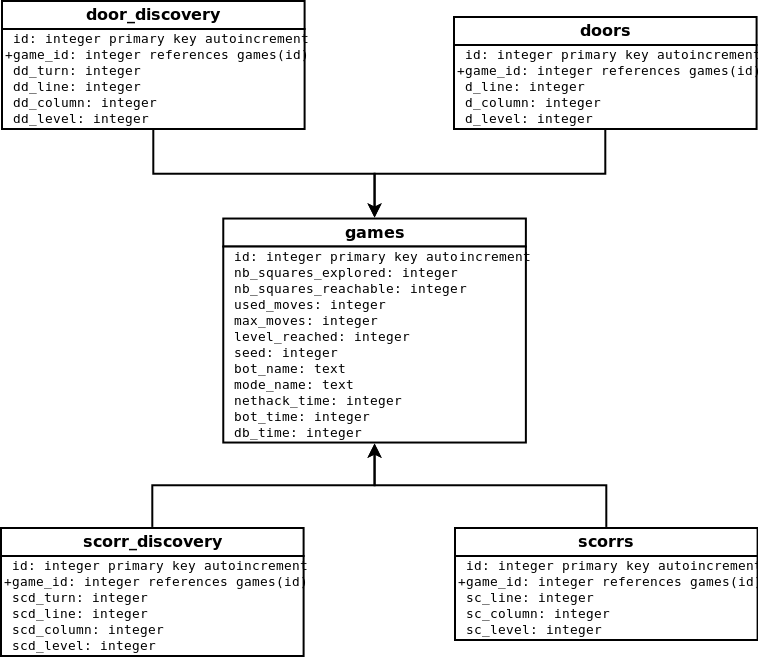
\includegraphics[width=\textwidth]{schema.png}}
	\caption{\label{fig:schema} Schéma de la base de données utilisée.}
\end{figure}
Une vue
fournissant certains détails supplémentaires \footnote{Nombre de portes
secrètes, nombre de portes secrètes trouvées, nombre de couloirs secrets et
nombre de couloirs secrets trouvés.} est aussi disponible afin de faciliter
l'utilisation de la base de données.
\\
Nous avons choisi d'utiliser une base de données {\em sqlite3}, celle-ci étant
assez simple à interfacer avec du {\em C}, mais aussi à interroger directement
par ligne de commande. Le grand avantage pour notre situation est aussi que les
bases de données {\em sqlite3} se présentent sous la forme d'un unique fichier,
celui-ci n'étant pas trop volumineux, il était parfaitement concevable de nous
échanger les bases de données de manière simple.
%TODO Parler des .def etc?


\subsubsection{Scripts de génération de graphiques}

Afin de visualiser les performances des différents bots, de pouvoir les comparer
facilement et de pouvoir vérifier statistiquement des propriétés de nethack,
nous avons mis en place des scripts permettant de générer de façon automatique
différents graphiques à partir d'une base de données. Ces graphiques se séparent
en trois catégories principales :
\begin{itemize}
\item Les graphiques permettant de mieux évaluer la répartition des performances
  des bots. Ceux-ci permettant entre autre de détecter que le bot ne fonctionne
  pas comme souhaité.
\item Les graphiques permettant de comparer les bots entre eux. Ceux-ci
  représentent la performance des bots sur un critère particulier en fonction du
  nombre maximal de mouvements autorisés. Ils permettent de départager les
  différentes stratégies par rapport à des objectifs.
\item Les graphiques analysant des données qui ne sont pas spécifiques au bot
  afin de permettre de vérifier certaines propriétés ou d'observer la
  distribution de certains événements aléatoires propres à nethack.
\end{itemize}
Tous les graphiques sont générés à l'aide de {\em gnuplot}, le type de sortie
peut facilement être modifié et permet ainsi de convenir à ce qui est attendu

\paragraph{Graphiques analysant un bot}

\subparagraph{Exemple}
Nous avons écrit un script permettant de générer un grand nombre de graphiques
indiquant la répartition des performances du bot. Celui-ci génère un graphique
par triplet
$\{\text{Bot},\text{Nb mouvements autorisés},\text{Caractéristique} \}$, il
faut par conséquent faire attention car suivant la base de données utilisée,
le temps de génération peut être conséquent. Voici un exemple d'un des graphes
produits par ce script.

\begin{figure}[H]
  \center{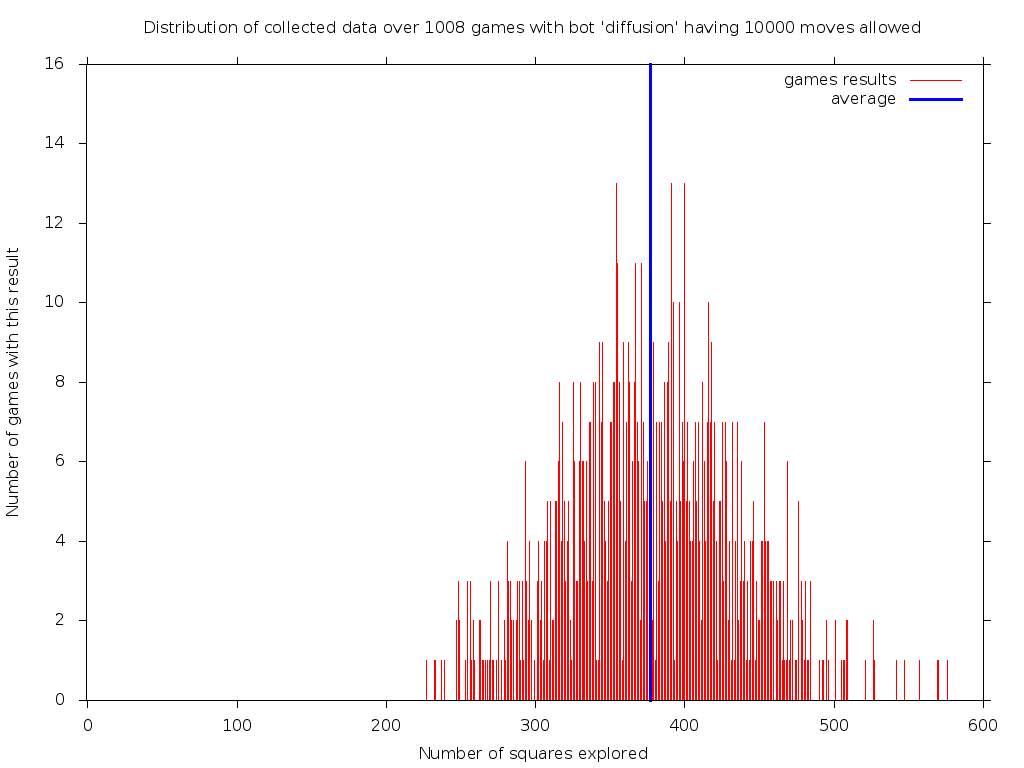
\includegraphics[width=\textwidth]{m_10000_nb_squares_explored.png}}
	\caption{\label{fig:impulse_graph} Un exemple de graphique montrant la
    répartition des performances}
\end{figure}

\subparagraph{Observation de caractéristiques du jeu}
Il est important de noter que ce script ne génère pas des graphes de répartition
que pour les performances du bot, il génère un graph similaire pour le résultat
maximal de chaque caractéristique, ce qui permet aussi d'observer la répartition
de celle-ci pour nethack. Nous avons ainsi constaté que la plupart des
caractéristiques \footnote{Nombre de portes secrètes présentes sur un niveau,
nombre de couloirs secrets présents sur un niveau et nombre de cases
explorables} que nous avons observées suivaient une distribution ayant en tout
cas l'apparence d'une gaussienne.
\\
Suivant les objectifs du bot, on peut donc imaginer qu'un bot se serve des
résultats obtenus afin de déterminer s'il est probable qu'il existe une autre
salle cachée où s'il a déjà tout visité. Cet aspect sera approfondi dans la
section {\em Analyses}.

\subparagraph{Observation de caractéristiques du bot}
Si l'exemple donné ci-dessus présente le nombre de cases explorées par le bot
comme suivant une gaussienne, certains aspects de répartition peuvent donner
plus d'informations, comme c'est le cas sur ce graphique.

\begin{figure}[H]
  \center{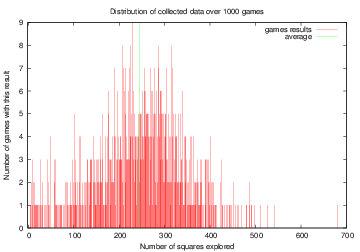
\includegraphics[width=0.5\textwidth]{nb_squares_explored.png}}
  \caption{\label{fig:nb_squares_explored} Un exemple de graphique montrant un
  dysfonctionnement du bot.}
\end{figure}

Le fait que la répartition des résultats ne suit pas une gaussienne n'est pas
forcément flagrant, en revanche, on distingue un nombre non négligeable de
parties ayant un nombre de cases explorées inférieur à 50, ce qui est très
faible en comparaison de la moyenne. En observant plus en détail une des
parties ayant obtenu un tel résultat, nous nous sommes rendus compte que le
problème venait du fait que les portes ne s'ouvraient plus, ce qui était dû à
une légère erreur lors d'une modification du noyau. Ces graphiques peuvent
donc aussi servir à détecter des dysfonctionnements lors de modifications du
noyau.

\paragraph{Graphiques comparant des bots}
Afin de comparer les performances des bots dans différents domaines, nous
avons écrit un script générant des graphiques permettant de visualiser
facilement les différences de résultats entre les différents bots. Celui-ci
génère un graphe par caractéristique observée, permettant ainsi de réduire le
nombre de manipulations à effectuer.

\begin{figure}[H]
  \center{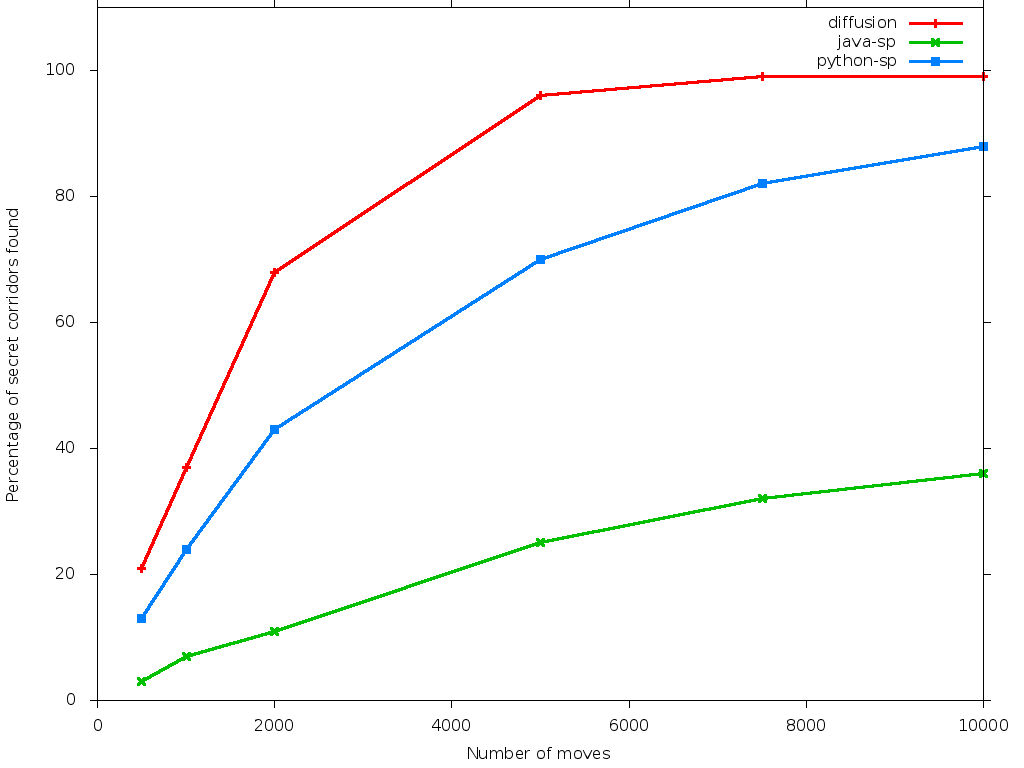
\includegraphics[width=\textwidth]{graph_percent_scorrs_found.png}}
  \caption{\label{fig:move_graph} Un exemple de graphique comparant des bots}
\end{figure}

Il est possible de donner des noms différents au même bot au fur et à mesure
qu'il évolue, en ajoutant des données à la même base, ainsi il est possible de
mesurer l'amélioration des performances. Ce raisonnement s'applique aussi à
des modifications de paramètres sur le bot diffusion par exemple, ce qui
pourrait permettre par exemple de faire de l'apprentissage sur les différents
paramètres afin de trouver les valeurs idéales. Le problème du bot diffusion
étant que lancer de nombreuses parties demande un temps d'exécution important.

\paragraph{Graphiques analysant la distribution des portes et couloirs secrets}
Afin d'observer des informations sur la distribution des portes et couloirs
secrets, nous avons créé des scripts permettant de visualiser le nombre de
portes secrètes ou de couloir secrets pour chaque emplacement. La possibilité de
visualiser l'information en deux ou en trois dimensions est fournie. En deux
dimensions, deux graphiques sont disponibles, l'un représentant le nombre
d'éléments trouvés en fonction de la ligne, l'autre en fonction de la colonne.
Seul le graphique en trois dimensions permet de visualiser les deux
simultanément. S'appuyant sur {\em gnuplot}, les scripts générant les graphiques
en trois dimensions proposent un mode interactif permettant de changer l'angle
de vue.

\begin{figure}[H]
  \center{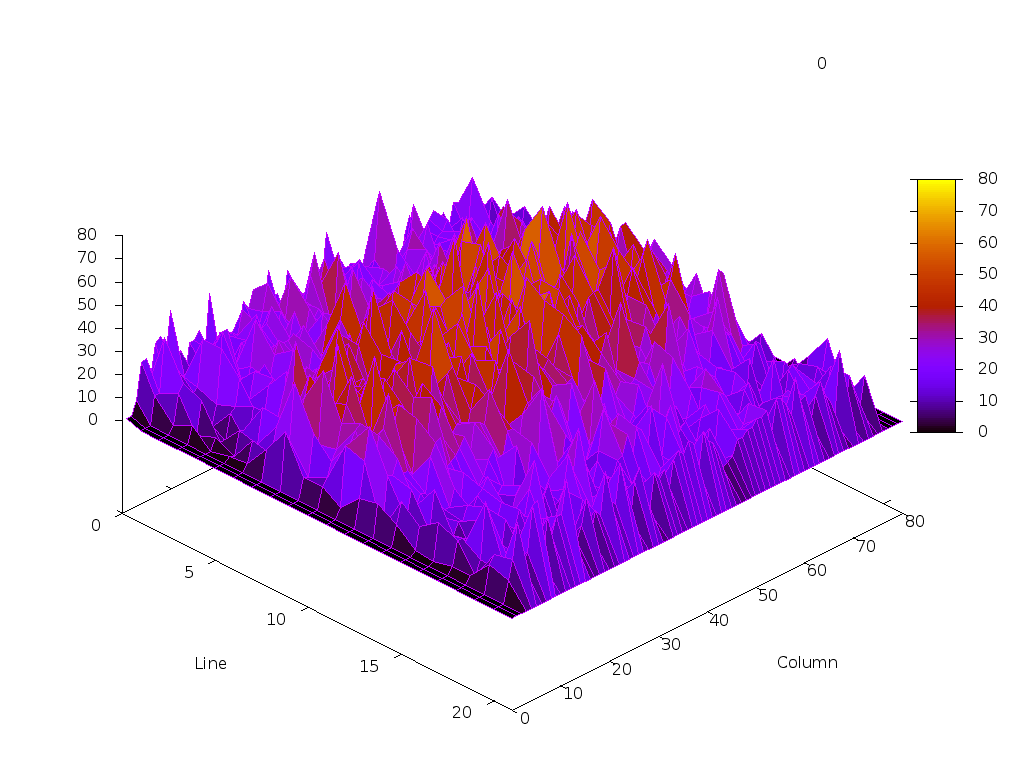
\includegraphics[width=\textwidth]{3d_exemple.png}}
  \caption{\label{fig:move_graph} Aperçu de la visualisation du nombre de
    couloirs secrets en fonction de la position.}
\end{figure}

L'utilité exacte de ce type de graphiques sera approfondie dans la partie
{\em Analyses}.


\section{Analyses}

Le code fourni nous a permis non seulement de comparer l'efficacité des bots
existants dans différents modes de jeu, mais aussi d'analyser certains aspects
de nethack. Pour tous ces tests, nous n'avons finalement utilisé qu'un seul
ensemble de patchs, celui associé à l'exploration. Les modifications de
l'expérience de jeu par rapport à la version originale de nethack sont les
suivantes :

\begin{itemize}
\item Désactivation de la faim.
\item Désactivation de tous les monstres.
\item Désactivation des objets normaux et spéciaux.
\item Désactivation des pièges\footnote{Si le nombre de piège a été grandement
  réduit, il reste malgré tout des portes piégées qui tuent ou assomment parfois
  le personnage lorsque l'on descend dans les niveaux}
\item Disparition des portes lorsqu'elles sont ouvertes ou défoncées
  \footnote{Ce patch s'est révélé pratique afin de simplifier la distinction
    entre les murs et les portes ouvertes, en effet, cela permet de ne pas
    inclure les portes ouvertes dans le protocole.}.
\end{itemize}

\subsection{Recherche d'éléments secrets}
Le but de ce mode est de retrouver toutes les portes secrètes et les couloirs
secrets présents dans le niveau initial. Une des contraintes est donc de ne pas
descendre d'étage. Les descentes accidentelles semblent effectivement avoir été
évitées étant donné que sur plus de 18'000 parties jouées dans ce mode par trois
bots différents, aucune n'a un niveau maximal atteint supérieur à 1.
\\
Nous avons aussi observé le pourcentage de cases visitées, même si ce n'était
pas un but directement affiché, après plusieurs expériences, celle-ci semble
naturellement suivre la même tendance que les deux autres.
\\
Afin de présenter des données à jour, nous avons lancé dans la dernière semaine
plus de 18'000 parties dont les résultats ont servis à générer les graphiques
qui seront présentés par la suite. Pour chacun de ceux-ci, tous les points
représentent la moyenne des résultats sur au moins 1000 parties. Cet ordre de
grandeur nous permet de réduire fortement le risque que les données présentées
soient biaisées par un mauvais échantillons.
\\
Sur tous les graphiques de comparaisons, {\em java-sp} sert de référence, ce bot
étant totalement aléatoire, il donne un exemple des résultats obtenus par un bot
ne présentant aucune intelligence mais qui ne risque pas de tomber dans des
boucles infinies.

\subsubsection{Pourcentage de portes secrètes trouvées}

\begin{figure}[H]
  \center{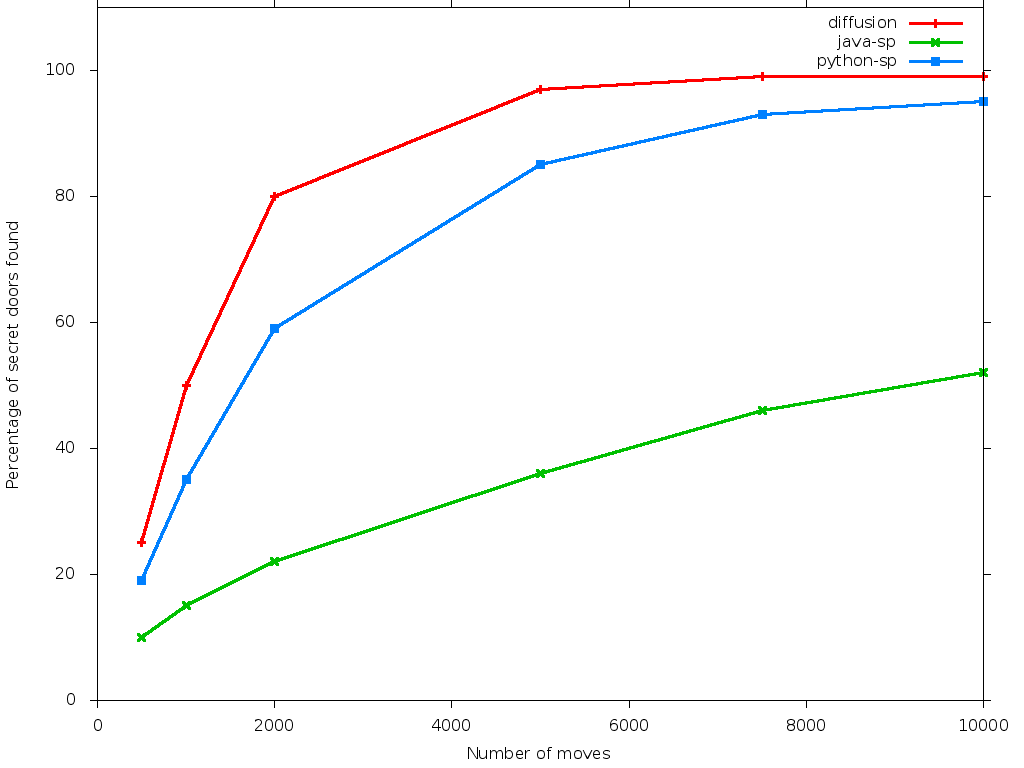
\includegraphics[width=\textwidth]{graph_percent_sdoors_found.png}}
  \caption{\label{fig:sdoors_found} Pourcentage de portes secrètes trouvées en
    fonction du nombre de mouvements autorisé}
\end{figure}

Les deux bots {\em évolués} ont des performances nettement meilleures que le bot
aléatoire, ce qui est assez rassurant sur leur fiabilité. Cette différence
montre aussi que même si le bot aléatoire augmente son pourcentage de détection
lorsque le nombre maximal de mouvements augmente, il nécessitera un nombre de
mouvement bien plus conséquent pour découvrir la moitié des portes secrètes.
\\
Bien que le bot {\em diffusion} trouve les portes plus rapidement que
{\em python-sp}, cette différence ne vaut pas nécessairement le surcoût engendré
par la différence de complexité asymptotique. Les données présentées ici
permettent néanmoins de pouvoir orienter son choix en connaissance de cause.

\subsubsection{Pourcentage de couloirs secrets trouvée}

\begin{figure}[H]
  \center{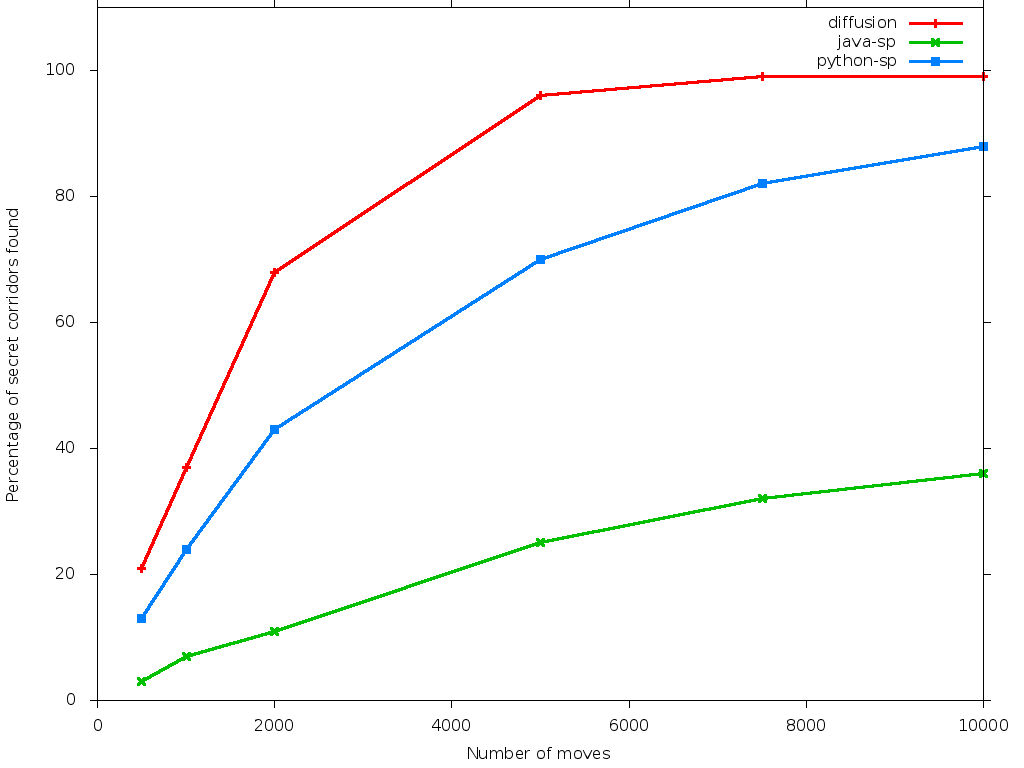
\includegraphics[width=\textwidth]{graph_percent_scorrs_found.png}}
  \caption{\label{fig:scorrs_found} Pourcentage de couloirs secrets trouvés en
    fonction du nombre de mouvements autorisé}
\end{figure}

La tendance générale ressemble beaucoup à celle obtenue pour les portes
secrètes, cependant en s'attardant un peu plus sur le graphique, on s'aperçoit
que la différence entre les bots est plus importante. Ceci peut être expliqué
par le fait que le bot {\em diffusion} accorde une priorité plus grande aux
couloirs aboutissant à des cul-de-sac et que le bot {\em python-sp} une fois
bloqué aura tendance à faire de nombreuses recherches, %TODO verify by Benoit
en revanche, le bot aléatoire aura tendance à faire très peu de recherche dans
ces emplacements là\footnote{Cette différence est illustrée dans la partie
{\em Aperçu du nombre de visites sur chaque case}.}.
\\
On peut constater qu'effectivement le bot aléatoire découvre moins de 30\% des
couloirs secrets avec 10'000 mouvements alors qu'il découvrait plus de 50\% des
portes secrètes avec cette même limite.

\subsubsection{Pourcentage de cases explorées}

\begin{figure}[H]
  \center{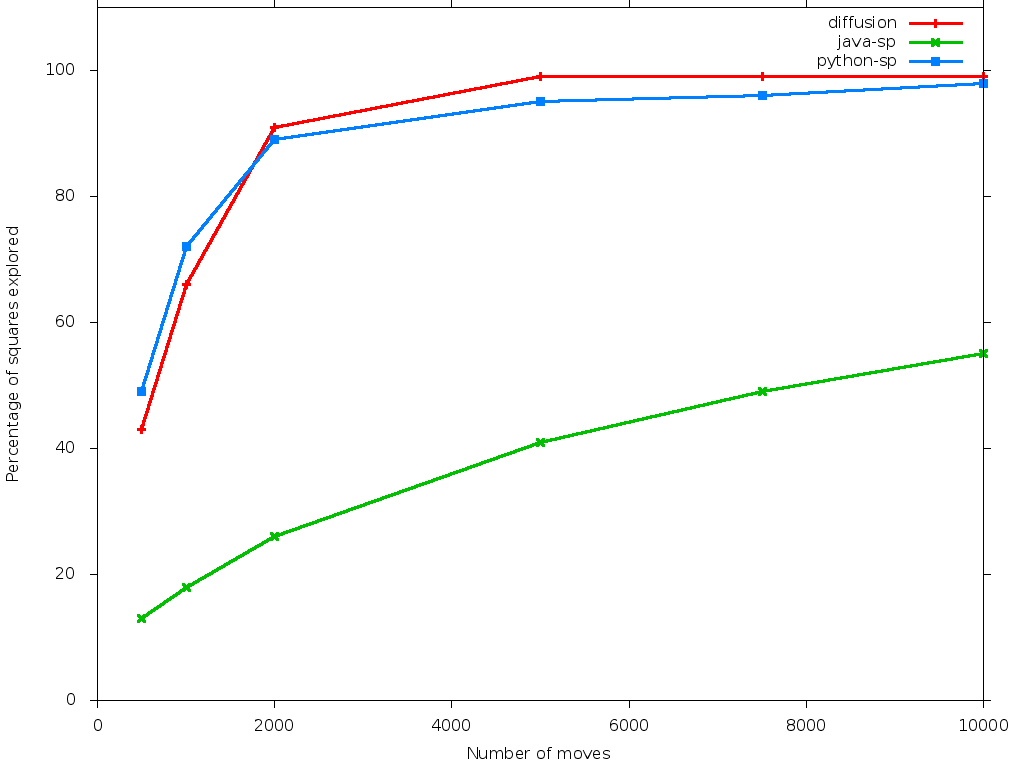
\includegraphics[width=\textwidth]{graph_percent_explored.png}}
  \caption{\label{fig:squares_explored} Pourcentage de cases explorées en
    fonction du nombre de mouvements autorisé}
\end{figure}

La différence entre le bot aléatoire et les autres est aussi grande que pour les
deux catégories précédentes, cependant on peut observer que lorsque le nombre de
mouvements autorisé est faible, le bot {\em python-sp} explore plus de cases que
le bot {\em diffusion}. Cette différence s'explique assez facilement grâce aux
différences de stratégie. Le bot {\em diffusion} n'a pas tendance à explorer
toutes les cases à portée étant donné qu'elles ne sont pas toutes susceptibles
d'être à proximité d'un couloir secret ou d'une porte secrète \footnote{À
  nouveau, observer la visualisation de l'exploration du niveau permet de s'en
  rendre compte rapidement}. Cette tendance s'inverse à un moment donné,
sûrement lorsque le bot {\em python-sp} est bloqué car il doit découvrir une
porte secrète ou un couloir secret pour progresser tandis que le bot diffusion a
découvert toutes les salles. Si l'on souhaite améliorer les performances du bot
{\em diffusion} pour cette caractéristique, il suffit à priori de changer le
score attribué à la découverte d'une nouvelle case\footnote{Celui-ci étant
négligeable dans la version utilisée pour les parties concernées par ce
graphique}.

\subsection{Descente dans les niveaux}

TODO Données manquantes.

\subsection{Évaluation des bots}
Pour un temps de calcul du même ordre que le bot aléatoire, le bot
{\em python-sp} offre une qualité d'exploration incomparablement supérieure.
Cependant, il n'est pas fait pour être adapté à des changements d'objectifs
rapidement contrairement au bot {\em diffusion} qui obtient des scores
d'exploration élevés tout en permettant de changer les buts très facilement. Ces
avantages ont en revanche un coût en complexité très élevé \footnote{ Il devrait
néanmoins être possible d'améliorer grandement le temps d'exécution de ce bot
avec des solutions algorithmiques plus poussées.}.

\subsection{Éléments indépendants des bots}
Certaines de nos analyses ne concernaient pas des bots, mais le jeu lui-même. En
effet, bien que le jeu se base sur un générateur aléatoire, cela ne signifie pas
que toutes les positions ont la même probabilité de contenir une porte par
exemple. Pour répondre à ce type de question, le bot utilisé importe peu, il
n'est même pas nécessaire d'utiliser un bot à priori, il suffit de générer la
carte.
\\
Les éléments que nous avons choisis d'observer sont la probabilité qu'une case
contienne une porte secrète ou un couloir secret en fonction de leurs positions.

\paragraph{Événements dépendants}
Avant de présenter certains résultats que nous avons obtenus, il est important
de préciser quelques points théoriques. Pour ce faire, nous allons utiliser les
notations suivantes :
\begin{itemize}
\item $C_{l,c}$ :
  représente le contenu de la case à ligne $l$ et à la colonne $c$.
\item $A_{l,c}$ :
  représente {\em l'apparence}\footnote{L'apparence signifie ce que perçoit le
    joueur, il peut par exemple percevoir un mur à une position alors que le
    contenu est une porte secrète.} de la case à ligne $l$ et à la colonne $c$.
\item $M$ :
  représente le type {\em mur}.
\item $PS$ :
  représente le type {\em porte secrète}.
\item $CS$ :
  représente le type {\em couloir secret}.
\end{itemize}

Les données qui sont acquises vont donner une estimation pour tout couple
$\{l,c\}$ de $P(C_{l,c} = PS)$ et de $P(C_{l,c} = CS)$. Cependant, ces estimations
ne fournissent pas un résultat directement utilisable pour les bots, car la
probabilité que le contenu soit d'un type donné dépend du type apparent.
\footnote{$P(C_{l,c} = CS | A_{l,c} = M) \neq P(C_{l,c} = CS)$ de manière flagrante
  car si l'apparence est un mur, le contenu ne peut pas être un couloir secret}
\\
Cette dépendance des variables implique que les valeurs qui nous intéressent
réellement sont celles du type $P(C_{l,c} = ... | A_{l_c} = ...)$. Celles-ci ne
peuvent pas être obtenues à partir de la base de données que nous avons
utilisées car il est nécessaire de conserver une trace de l'apparence. En
revanche, à partir du code fournit, il est possible d'apporter des modifications
permettant de calculer ces probabilités.
\\
Bien que les graphiques obtenus ne soient pas directement applicables aux bots,
ils présentent tout de même un intérêt.

\paragraph{Emplacement des portes secrètes}

\begin{figure}[H]
  \center{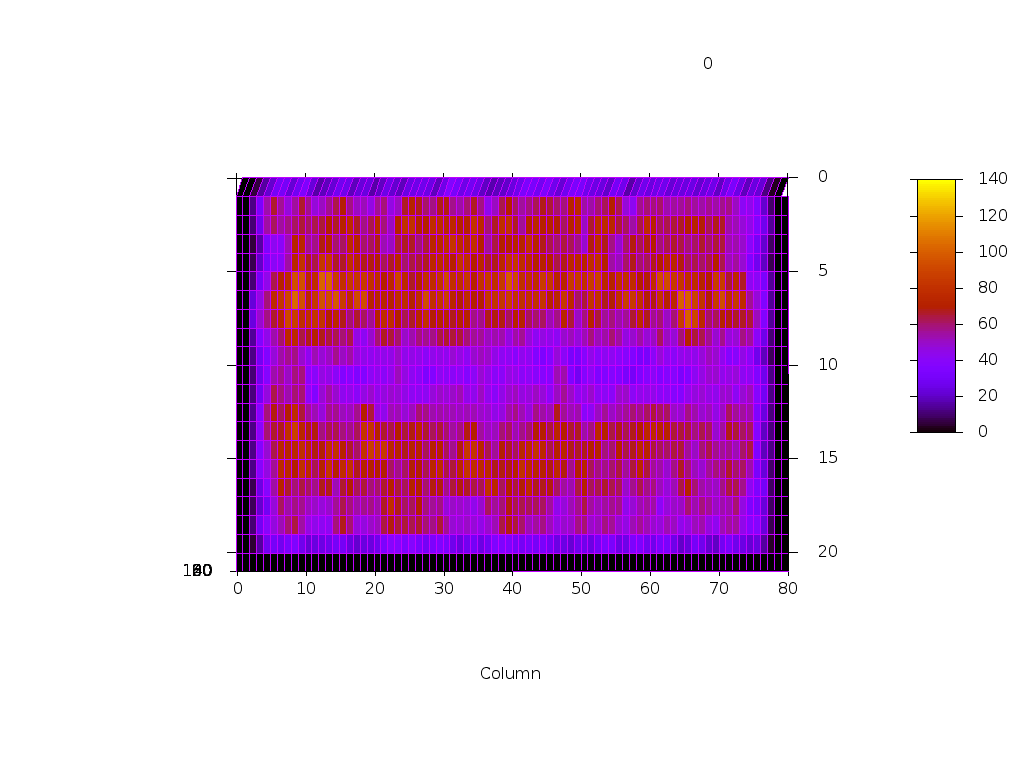
\includegraphics[width=\textwidth]{3d_sdoors_graph.png}}
  \caption{\label{fig:3d_sdoors_graph} Nombre de portes secrètes en fonction
    de la ligne et de la colonne}
\end{figure}

Ce graphique montre incontestablement que $P(C_{l,c} = PS)$ n'est pas indépendant
de $\{l,c\}$. Cette information encourage à approfondir les recherches
mentionnées ci-dessus, car il semble probable qu'il y ait des informations
utilisables si l'on suit la démarche indiquée au paragraphe précédent.
\\
De plus, bien que la probabilité semble être plus élevée suivant deux bandes
horizontales et faible aux alentours de la ligne 10, ce phénomène ne s'observe
pas par rapport aux colonnes. Les emplacements à l'intérieur de ces bandes ne
semblent pas équiprobables et la différence de probabilité y semble même assez
élevée. La probabilité de trouver une porte secrète dans les bords semble nulle.

\paragraph{Emplacement des couloirs secrets}

\begin{figure}[H]
  \center{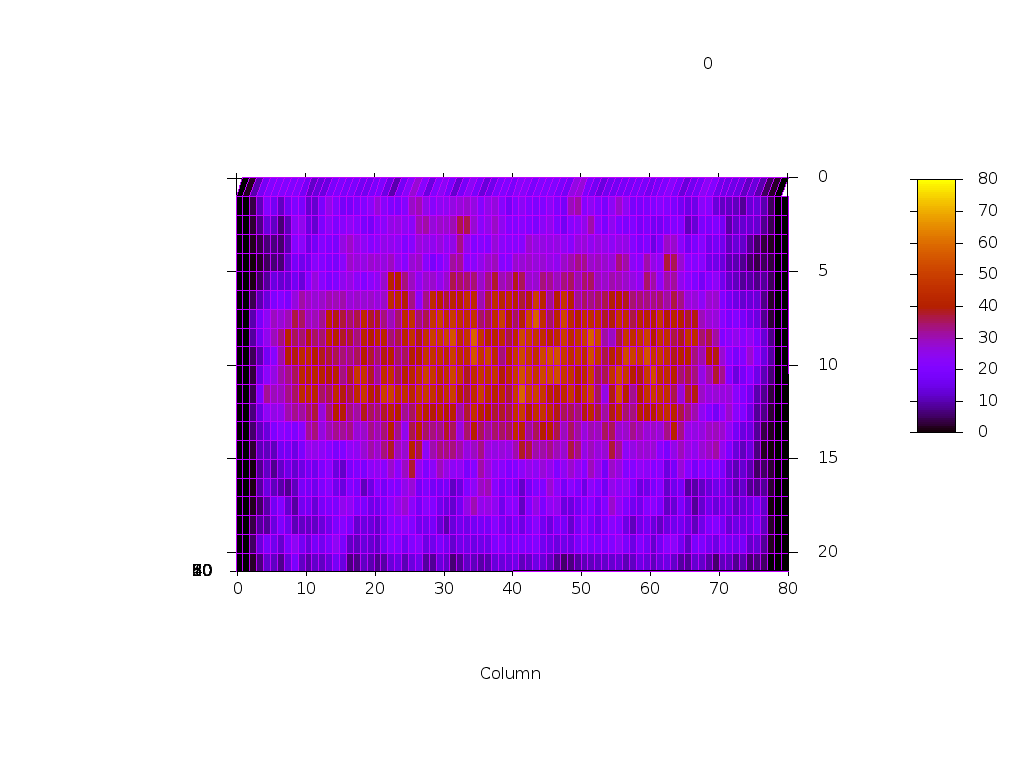
\includegraphics[width=\textwidth]{3d_scorr_graph.png}}
  \caption{\label{fig:3d_scorr_graph} Nombre de couloirs secrets en fonction
    de la ligne et de la colonne}
\end{figure}

Ce graphique indique que les colonnes au bord de la cartes sont très peu
susceptibles de contenir des couloirs secrets tandis que la probabilité que les
lignes aux bord de la carte en contiennent n'est pas négligeable. On peut aussi
voir que les lignes centrales ont bien plus de chances de contenir un couloir
secret que celles du bord\footnote{Peut-être est-ce parce qu'il y a simplement
plus de couloirs au centre de la pièce que dans les bords, comme évoqué dans le
paragraphe {\em Événements indépendants}}.
\\
Ces observations encouragent aussi à approfondir les recherches générales sur
Nethack afin de pouvoir les utiliser pour améliorer des bots.

\subsection{Problème simplifié : sortie d'une salle}

Afin d'étudier le problème de la recherche des portes secrètes de façon plus
théorique, nous avons réduit le nombre de paramètres aléatoires et simplifié
volontairement la situation.
\\
Dans ce niveau particulier :
\begin{itemize}
\item Le personnage apparaît au milieu d'une salle de $10$ lignes par $10$
  colonnes.
\item La salle est entourée de murs et un seul de ceux-ci contient une porte
  secrète.
  \footnote{Il y a {\em exactement} une porte secrète}
\item Tous les emplacements ont la même probabilité de contenir la porte
  secrète.
  \footnote{Ce point a été vérifié par l'expérience en générant un grand nombre
    de parties et en observant la répartition des portes secrètes}
\item Effectuer une recherche dans une des cases adjacentes au mur contenant la
  porte secrète a une probabilité de révéler celle-ci de $\frac{1}{7}$.
\item Le personnage est placé aléatoirement dans la pièce.
\end{itemize}

Ces conditions sont assurées par l'utilisation d'un patch supplémentaire, venant
s'additionner à ceux mentionnés dans la partie {\em Analyses}.
\\
Voici un aperçu de l'apparence de la pièce, les carrés violets étant ceux où la
porte secrète peut se trouver.

\begin{center}
  \begin{tikzpicture}[scale=.5]
    % Drawing Walls part
    \foreach \x in {1,...,10}{
      \draw [fill=violet] (\x,  0) rectangle (\x + 1,  1);
      \draw [fill=violet] (\x, 11) rectangle (\x + 1, 12);
    }
    \foreach \y in {1,...,10}{
      \draw [fill=violet] ( 0, \y) rectangle ( 1, \y + 1);
      \draw [fill=violet] (11, \y) rectangle (12, \y + 1);
    }
    % Drawing internal grid
    \foreach \x in {1,...,10}{
      \foreach \y in {1,...,10}{
        \draw (\x,\y) rectangle (\x + 1,\y + 1);
      }
    }
  \end{tikzpicture}
\end{center}

Être certain d'avoir la meilleure stratégie étant trop complexe à nos yeux, nous
avons décider de chercher plutôt à définir une borne inférieure. Une fois
celle-ci obtenue, il est donc possible de la comparer aux résultats obtenus par
les bots. La différence entre ces deux résultats pourra être réduite de deux
façons :
\begin{itemize}
\item En augmentant la borne inférieure par des résultats théoriques.
\item En diminuant la borne supérieure par des modifications du bot.
\end{itemize}

\subsubsection{Approche théorique}

\paragraph{Dominer la pièce :}
Il est possible de fixer certaines cases où les recherches seront effectuées en
cherchant à minimiser ce nombre de cases, tout en ayant à portée tous les murs.
\footnote{Cette notion est comparable à la domination en théorie des graphes,
  les différences principales étant que l'on ne peut pas choisir n'importe quel
  sommet, certains sommets étant interdits et qu'il n'est pas nécessaire de
  dominer tous les sommets, mais uniquement les interdits.}
\\
En colorant en orange les cases où les recherches seront effectuées, et en
indiquant la portée des recherches par les carrés oranges transparents, le
résultat obtenu est le suivant :

\begin{center}
  \begin{tikzpicture}[scale=.5]
    % Drawing Walls part
    \foreach \x in {1,...,10}{
      \draw [fill=violet] (\x,  0) rectangle (\x + 1,  1);
      \draw [fill=violet] (\x, 11) rectangle (\x + 1, 12);
    }
    \foreach \y in {1,...,10}{
      \draw [fill=violet] ( 0, \y) rectangle ( 1, \y + 1);
      \draw [fill=violet] (11, \y) rectangle (12, \y + 1);
    }
    % Drawing internal grid
    \foreach \x in {1,...,10}{
      \foreach \y in {1,...,10}{
        \draw (\x,\y) rectangle (\x + 1,\y + 1);
      }
    }
    % Coloring squares and ranges of research
    \foreach \x in {1,4,7,10}{
      \draw [fill=orange] (\x,  1) rectangle (\x + 1,  2);
      \draw [fill=orange] (\x, 10) rectangle (\x + 1, 11);
      \draw [ultra thick, orange] (\x - 0.5, 0.5) rectangle (\x + 1.5,  2.5);
      \draw [ultra thick, orange] (\x - 0.5, 9.5) rectangle (\x + 1.5, 11.5);
    }
    \foreach \y in {1,4,7,10}{
      \draw [fill=orange] ( 1, \y) rectangle ( 2, \y + 1);
      \draw [fill=orange] (10, \y) rectangle (11, \y + 1);
      \draw [ultra thick, orange] (0.5, \y - 0.5) rectangle ( 2.5, \y + 1.5);
      \draw [ultra thick, orange] (9.5, \y - 0.5) rectangle (11.5, \y + 1.5);
    }
  \end{tikzpicture}
\end{center}
Il est assez évident qu'il est impossible de recouvrir chaque cases contenant
potentiellement une porte avec moins de carrés, car tous les coins\footnote{Ce
sont eux qui sont a portées du plus grand nombre de sommets à dominer.} sont
utilisés et aucune case n'est à portée de deux emplacements de recherches.

\paragraph{Évolution des probabilités :}
Si l'on ignore le coût des déplacements, prenant en compte uniquement les coûts
de recherche, le meilleur comportement semble être de commencer par chercher
dans les coins et d'utiliser ensuite les autres emplacements, ceci en
considérant qu'ils ont tous le même nombre de recherche au début. Il n'est en
revanche pas évident de déterminer si un coin sur lequel $n+1$ recherches ont
été effectuées a une chance plus élevée d'être à proximité d'une porte secrète
qu'un bord où $n$ recherches ont été effectuées.
\\
La probabilité initiale de découvrir une porte est égale à 
$\frac{1}{40} \times \frac{1}{7}$, la probabilité initiale de trouver une porte
secrète dans un coin est donc de : $4 \times \frac{1}{40} \times \frac{1}{7}$.
Lorsque des recherches sont effectuées, la partie représentant la probabilité de
trouver la porte secrète en sachant que l'on a cherché au bon endroit ne sera
pas modifiée ($\frac{1}{7}$). En revanche, la probabilité que la porte secrète
soit sur une case spécifique dépendra du nombre et de l'emplacement des
recherches déjà effectuées\footnote{Ce problème est semblable au fameux
problème de Mounty Hall, le point clé étant que l'on {\em sait} qu'il y a 
{\em exactement} une porte secrète parmi les 40 cases de murs}. Une intuition de
ce fait peut être donnée par l'exemple suivant : 10'000 recherches ont été
effectuées sur chacun des emplacements de recherches excepté sur celui se
situant en haut à gauche où aucune recherche n'a été effectuée, la probabilité
qu'une recherche sur cette case aboutissent est clairement de plus de 
$\frac{1}{10}$.
\\
Afin de présenter une preuve de cette différence de probabilité, nous allons
simplifier ce problème en considérant qu'il existe uniquement deux emplacements
où la porte secrète peut se trouver et que chaque recherche ne peut être à
portée que d'un seul d'entre eux.\\
On considère les notations suivantes :
\begin{itemize}
\item $Pos(P)$ est la position de la porte.
\item $T$ signifie que la porte a été trouvée.
\item $PT$ signifie que la porte n'a pas été trouvée.
\end{itemize}
Après une recherche en position $1$, on obtient l'arbre de probabilité suivant:

% Set the overall layout of the tree
\tikzstyle{level 1}=[level distance=3.5cm, sibling distance=3.5cm]
\tikzstyle{level 2}=[level distance=3.5cm, sibling distance=2cm]

% Define styles for bags and leafs
\tikzstyle{bag} = [text width=4em, text centered]
\tikzstyle{end} = [circle, minimum width=3pt,fill, inner sep=0pt]
\begin{center}
  \begin{tikzpicture}[grow=right, sloped]
    \node[bag] {Overall}
    child {
      node[bag] {Porte en $1$}        
      child {
        node[end] {}
        edge from parent
        node[above] {$T$}
        node[below]  {$\frac{1}{7}$}
      }
      child {
        node[end] {}
        edge from parent
        node[above] {$NT$}
        node[below]  {$\frac{6}{7}$}
      }
      edge from parent 
      node[above] {$Pos(P) = 1$}
      node[below]  {$\frac{1}{2}$}
    }
    child {
      node[bag] {Porte en $2$}
      child {
        node[end] {}
        edge from parent
        node[above] {$NT$}
        node[below]  {$1$}
      }
      edge from parent         
      node[above] {$Pos(P) = 2$}
      node[below]  {$\frac{1}{2}$}
    };
  \end{tikzpicture}
\end{center}

Si la première recherche a terminée sans que la porte n'ait été trouvée, les
nouvelles probabilités peuvent être aisément calculées :
\begin{itemize}
\item $P(Pos(P) = 1) = \frac{\frac{1}{2} \times \frac{6}{7}}
                            {\frac{1}{2} \times \frac{6}{7} +
                             \frac{1}{2}}
                     = \frac{6}{13}$
\item $P(Pos(P) = 2) = \frac{\frac{1}{2}}
                            {\frac{1}{2} \times \frac{6}{7} +
                             \frac{1}{2}}
                     = \frac{7}{13}$
\end{itemize}

\paragraph{Calcul de la probabilité :}
Nous avons déjà démontré que deux emplacements ne sont plus équiprobables si
plus de recherches ont été effectués sur l'un que sur l'autre. Il est aussi
évident que la méthode présentée ci-dessus sera très difficile à appliquer sur
un grand nombre de recherches. C'est pour cette raison que nous avons développé
une autre approche, permettant de calculer les probabilités de façon plus simple
et aussi beaucoup plus rapide pour un ordinateur.\\
À partir de l'arbre de probabilité présentés précédemment, il est facile de voir
que la probabilité qu'une recherche soit fructueuse dépend uniquement de la
probabilité qu'une porte cachée se situe à portée de l'endroit où est effectuée
la recherche.
\\
Afin de résoudre ce problème dans un cas plus général, nous définissons
certaines notations :
\begin{itemize}
\item $W$ est l'ensemble des emplacements de recherches.
  $W = \{W_0,W_1, ... , W_{|W| -1} \}$
\item $R(W_k)$ représente le nombre de recherche faîtes sur l'emplacement $W_k$.
\item $V(W_k)$ représente le nombre de voisins de l'emplacement $W_k$
  susceptibles de contenir une porte secrètes.
\item $P(W_k = V)$ représente la probabilité que la porte secrète soit voisine
  de l'emplacement $W_k$.
\item $p$ est la probabilité de trouver une porte sachant qu'un de ses voisins
  contient la porte secrète.\footnote{$\frac{1}{7}$ dans le cas étudié ici.}
\end{itemize}

En accord avec les règles de probabilités, on définit donc la probabilité
qu'une recherche aboutisse ainsi :
$$P(W_k = V) = \frac{\text{cas favorables}(W_k)}{\text{cas possibles}}$$
Ces deux éléments peuvent être définis ainsi :
\begin{itemize}
\item $\text{cas favorables}(W_k) = V(W_k) * (1-p)^{R(W_k)}$
\item $\text{cas possibles} = \sum\limits_{k=0}^{|W| - 1}{V(W_k) * (1-p)^{R(W_k)}}$
\end{itemize}

On aboutit donc à la formule suivante pour définir la probabilité que la porte
soit à portée de l'emplacement $W_k$:
$$ P(W_k = V) = \frac{V(W_k) *(1-p)^{R_k}}{\sum\limits_{k=0}^{|W| - 1}{V(W_k) * (1-p) ^{R_k}}}$$
Comme $\text{cas possibles}$ n'est pas fonction de $k$, il est possible de
comparer l'intérêt de différentes cases uniquement en comparant les valeurs de
$\text{cas favorables}(W_k)$.
\\
Dans notre situation:
\begin{itemize}
\item Pour les coins, $V(W_k) = 4$.
\item Pour les bords, $V(W_k) = 3$.
\end{itemize}
Soient $k_1$ et $k_2$ tels que:
\begin{itemize}
\item $W_{k_1}$ est un coin.
\item $W_{k_2}$ est un bord.
\item $R(W_{k_1}) - R(W_{k_2}) = i$ avec $(1-p)^i = \frac{3}{4}$ ce qui implique
  que $i = \frac{\log(\frac{3}{4})}{\log(1-p)}$.\footnote{$i = 1,866$ dans notre
    cas.}
\end{itemize}
On obtient
$$\begin{array}{l c l}
\text{cas favorables}(W_{k_1})
&= &V(W_{k_1}) * (1-p)^{R(W_{k_1})}\\
&= &4 * (1-p)^{R(W_{k_2}) + i}\\
&= &4 * (1-p)^{R(W_{k_2})} * (1-p)^i\\
&= &4 * (1-p)^{R(W_{k_2})} * \frac{3}{4}\\
&= &3 * (1-p)^{R(W_{k_2})}\\
&= &V(W_{k_2}) * (1-p)^{R(W_{k_2})}\\
&= &\text{cas favorables}(W_{k_2})
\end{array}$$
Une implication importante de ce résultat est que pour un nombre de recherches
$n$, l'idéal sera que chaque coin ait eu $i$ recherches de plus que chaque bord.
De plus, la valeur de ce $i$ dépendra uniquement de $p$.

\paragraph{Minoration du nombre moyen de recherches :}
Si l'on désire minimiser le nombre moyen de recherches\footnote{Sans prendre du
  tout en compte le nombre de déplacements nécessaires}, il faut toujours
rechercher à l'emplacement ayant la plus haute probabilité d'être proche d'une
porte secrète. En effet, les chances que la porte soit trouvée sont maximales
pour un nombre de recherches $k$ si l'on se trouve dans un cas où les différents
emplacements de recherches ont des probabilités aussi proches que possibles.
\\
Nous noterons :
\begin{itemize}
\item $P_k$ : La probabilité de trouver la porte secrète en $k$ recherches au
  maximum.
\item $R_k$ : La probabilité de trouver la porte secrète en exactement $k$
  recherches.
\item $P(door)$ : La probabilité que la porte soit à l'emplacement de la
  recherche, cet emplacement est choisi comme étant le plus probable au moment
  de la recherche. Cette probabilité est calculée à l'aide de la formule trouvée
  précédemment.
\item $p$ : La probabilité de trouver la porte sachant qu'elle est voisine de la
  case où la recherche a été effectuée.
\end{itemize}
On obtient donc :
$$P_{k+1} = P_k + (1 - P_k) * P(door) * p$$
$$R_{k+1} = P_{k+1} - P_{k}$$
Quelque soit la stratégie choisie, il est donc évident que le nombre moyen de
recherches sera supérieur ou égal à $\sum\limits_{k=0}^{\infty} k * R_k$.
\\
Nous avons minoré cette valeur à l'aide d'un programme faisant l'addition de ces
termes tant que $R_k > 10^{-10}$ et nous avons obtenu environ $77,75$.

\subsubsection{Comparaison des résultats expérimentaux avec les valeurs
  théoriques}
La moyenne du nombre d'actions nécessaire au bot diffusion pour ouvrir la porte
sur 100 parties était de $158$, ce résultat est relativement proche de la borne
inférieure ($77,75$) si l'on prend en compte que la borne inférieure a été
calculée en ignorant totalement le coût des mouvements. En effet, afin
d'optimiser le nombre d'action moyen, le bot est obligé d'effectuer plusieurs
recherches sur un emplacement tandis que la stratégie utilisée pour calculer la
borne inférieure coûterait un nombre d'action très élevé en raison du nombre de
déplacements élevés qu'elle utilise.
\begin{figure}[H]
  \center{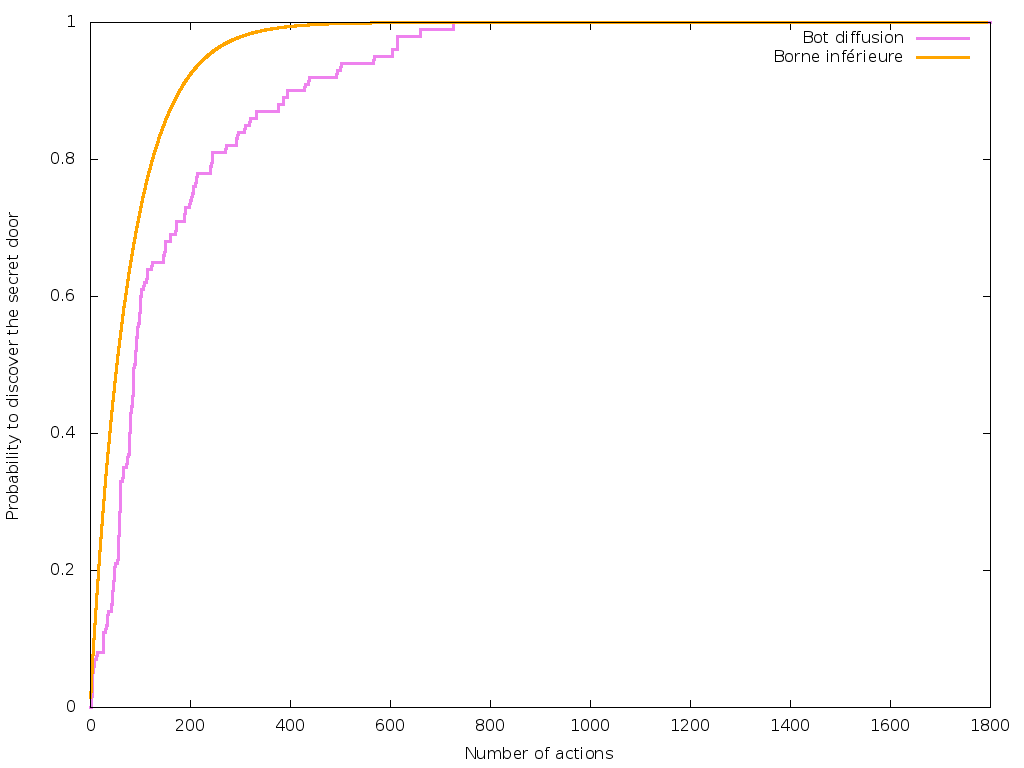
\includegraphics[width=\textwidth]{../images/compare.png}}
	\caption{\label{fig:compare} Graphique comparant les valeurs expérimentales du
  bot diffusion aux valeurs obtenues.}
\end{figure}

Une possibilité d'augmenter la borne inférieure pourrait être de minorer le
nombre de mouvement moyen. En effet, si l'on ignore totalement le coût des
recherches, il reste tout de même un nombre de mouvement non négligeable à
effectuer afin d'arriver à portée de la porte secrète (dont on ignore la
position).

\section{Documentation}
TODO: manuel d'utilisation, nombreux README, commentaires de
code (hors Doxygen), etc.

Doxygen a été utilisé afin de générer de façon automatique une documentation
destinée à de prochains développeurs à partir des commentaires placés dans le
code source des différents modules. Les "commentaires Doxygen" ont été
centralisés dans les fichiers d'en-tête contenus dans le dossier
\verb!include/!. Ces commentaires ont pour but de décrire le fonctionnement
global des modules et des fonctions mais servent aussi parfois à donner
certains détails d'utilisation ou avertir de certains comportements.

Les commentaires utilisés respectent le format suivant :
\begin{verbatim}
  /**
   * @brief Un résumé éventuel de ce que fait la fonction.
   *
   * Des détails sur la fonction.
   *
   * @param nom_parametre1 Description du premier paramètre éventuel.
   * @param nom_parametre2 Description du deuxième paramètre éventuel.
   */
\end{verbatim}

Le choix de rassembler tout les commentaires dans les fichiers d'en-tête n'est
pas anodin, cela facilite la lecture des commentaires dans le code source et
évite de 'polluer' les fichiers \verb!'.c'!, ce qui rendrait la navigation
plus difficile\footnote{Une autre pratique commune est le placement des
détails d'implémentation dans les fichiers \verb!'.c'! et la description de
l'utilité générale des fonctions dans les fichiers d'en-tête, cependant nous
n'avons pas privilégié cette approche ici.}.

\section{Tests}
Bien que nous n'ayons pas développés à proprement parler de tests unitaires au
cours de notre projet, nous n'avons pas négligé le fait de tester notre code. Au
fur et à mesure que notre projet avançait, les possibilités de tester
automatiquement le code et de le tester de manière fiable se sont améliorées.
Commençant par jouer des parties à la main pour vérifier l'absence d'erreur,
nous avons terminé par pouvoir comparer les distributions obtenues pour certains
bots avec les distributions attendues. Nous avons aussi pu collecter les graines
des parties qui posaient certains problèmes et les réutiliser pour vérifier que
nos interventions résolvaient effectivement les problèmes et que nos
modifications n'en faisaient pas réapparaître d'autres.
\paragraph{}
Afin de diagnostiquer les erreurs, nous avons entre autre pu nous servir du
{\em dummy client}, le principal défaut de tous ces tests étant qu'ils restent
des tests experts et ne peuvent donc pas être lancés par n'importe qui, validant
simplement les modifications.
\paragraph{}
Le {\em viewer} et les fichiers de logs nous ont aussi permis d'analyser des
dysfonctionnements qui provenaient des bots afin de les corriger. Le module de
visualisation de l'exploration {\em toTikz} permet aussi de mieux comprendre les
problèmes du bot.

\subsection*{Repérage des problèmes}
Utilisation du viewer pour comprendre ce qui ne va pas, utilisation de gdb,
quelques tentatives infructueuses de test de couverture (gcov), de profilage
(gprof) et mémoire (valgrind).

\section{Travail en équipe, organisation}

Bien que la conception du programme se soit effectuée au sein d'un groupe
de sept personnes, une séparation a eu lieu à mi-parcours, et c'est à trois que
s'est déroulée la phase de développement. Sans s'attarder sur les raisons de
cette séparation, il est nécessaire de l'évoquer afin de comprendre les
comparaisons qui seront faîtes.
\subsection{Utilisation de git :}
Lors de la première partie du projet, nous avions trois profils différents par
rapport à git :
\begin{itemize}
\item Ceux qui ne connaissait pas git et qui n'ont pas réussi à apprendre à s'en
  servir.
\item Ceux qui ne connaissait pas ou peu git et qui ont appréhendé réellement
  cet outil pendant cette phase.
\item Ceux qui connaissaient déjà git.
\end{itemize}
Au cours de la seconde partie en revanche, chacun de nous a pu apprendre à mieux
se servir de cet outil, se familiarisant plus avec la notion de branches et nous
avons réussi à comprendre de mieux en mieux les commits des autres, en essayant
de privilégier autant que possible des commits légers.
\\
L'utilisation des branches et des diff de git nous ont permis de créer les
patchs facilement sans interférer sur d'autres travaux. Nous avons pu réduire
rapidement le nombre de branche et travailler plus facilement les uns avec les
autres\footnote{Ceci étant peut-être dû à la taille de l'équipe.}. Cette façon
de travailler nous a permis de garder en permanence une branche fonctionnelle
tout en réglant certains problèmes en plusieurs commits.
\\
Lorsque nous modifions des détails dans le protocole, en ouvrant une autre
branche, chacun pouvait apporter les modifications nécessaires pour que tous les
bots acceptent ce changement.
\\
Nous avons aussi utilisé les {\em issues} github pour noter les problèmes qui
apparaissaient, entre autre afin de ne pas oublier qu'ils n'étaient pas traités.

\subsection{Différences d'organisation :}
Le fait que l'équipe ait été séparée en deux a modifié la nature du projet et
des difficultés auxquels nous avons du faire face. Il est en effet évident que
les problématiques de gestion de groupe qui se posent lors du développement à
sept personnes ne sont pas les mêmes qu'à trois.
\\
Durant la première partie du développement, bien que les tâches aient été
attribuées, l'équipe n'a pas fonctionné comme elle l'aurait dû. Nous avons
néanmoins pu planifier l'organisation. Les raisons de l'échec organisationnel de
cette première partie ne peuvent pas être définies aisément, mais il est
évident que notre groupe a pu beaucoup mieux fonctionner au cours de cette
seconde partie.
\\
Nous éprouvons tous une certaine frustration quand au fait que cette séparation
ait été nécessaire. En effet, malgré nos efforts, nous n'avons pas réussi à
faire fonctionner cette équipe et nous n'avons donc pas pu nous frotter
réellement aux difficultés qui apparaissent lors du travail dans des équipes
plus grandes. En revanche, pendant la seconde phase, nous avons bien réussi à
collaborer et à apprendre les uns des autres.

\subsection{Conventions}
Comme une partie de notre projet consiste à créer des patchs et à s'insérer dans
du code existant, il nous semblait naturel de chercher à adopter les conventions
utilisées par Nethack afin d'obtenir une certaine homogéneité dans celui-ci.
Les standards de codage variant à l'intérieur du projet et étant assez loin de
ceux auxquels nous sommes habitués, nous avons donc décidé trouver un juste
milieu en s'axant sur certains critères.
\begin{itemize}
\item {\em La langue :}\\
  Bien que le manuel et le rapport soient écrit en français,
  nous avons décidé de conserver l'anglais aussi bien pour le code et ses
  commentaires que pour les readme. Ce choix permet d'éviter de trop mélanger
  les appellations.
\item {\em L'utilisation des tabulations et des espaces :}\\
  Nethack mêlant les tabulations et les espaces, nous avons décidé de vérifier
  que quelque soit la taille d'affichage de la tabulation, nos patchs modifient
  le code de façon cohérente avec le code environnant. Pour le code extérieur à
  Nethack, nous avons choisi d'utiliser des tabulations pour marquer
  l'indentation et des espaces pour l'alignement, permettant ainsi aux
  utilisateurs de visualiser le code avec l'indentation qu'ils préfèrent, sans
  pour autant gâcher les alignements.
\item {\em La largeur de ligne maximale :}\\
  Dans la plupart de nos fichiers textes\footnote{Fichiers sources, README,
    fichiers tex, etc...} nous avons cherché à éviter que les lignes dépassent
  80 caractères, non seulement pour faciliter la lecture quelque soit l'outil
  utilisé, mais aussi pour permettre de visualiser plus facilement les
  différences apportées par des commits.
\item {\em Le nommage des variables et des fonctions :}\\
  Mis à part pour le code des bots en java qui suit un nommage CamelCase,
  nous avons décidé d'adopté un nommage à base d'underscore, comme utilisé dans
  nethack.
\item {\em Les accolades}\\
  Nous avons uniformisés le positionnement des accolades afin de faciliter la
  lecture du code.
\end{itemize}

Toutes les règles présentées ci-dessus sont celles que nous avons essayé de
respecter, néanmoins, nous avons plus considérés ces règles comme des sortes de
guides que comme une procédure stricte, il existe donc certainement des
exceptions à celles-ci dans le projet.

\section{Améliorations possibles}
Ce projet peut servir de base pour essayer différents bots d'exploration,
et pour valider leur efficacité par des expériences pratiques. Il peut aussi
être enrichi afin de présenter plus de fonctionnalités, de modes, de bots ou
encore d'étude théorique. Plusieurs de ces perspectives de continuation seront
décrites ici afin de donner des pistes à quiconque souhaiterait enrichir ce
projet.

\subsection{Fonctionnement de Nethack}
\subsubsection{Désactiver les niveaux spéciaux}
Aucun des patchs que nous avons créé ne modifie la génération des niveaux
original. Si ce fait ne nous a pas posé de problèmes lorsque les bots se
limitaient à l'exploration du premier niveau, cela s'est révélé être un problème
lorsque le but donné aux bots était de descendre dans le niveau le plus bas
possible. En effet, il se retrouvait toujours arrêté par des niveaux prédéfinis
qui présentait une spécificité\footnote{Pour certains niveaux, il était
nécessaire d'accomplir une quête pour pouvoir déverrouiller des portes, ces
interactions n'étant pas spécifiées par notre protocole, il était impossible que
le bot atteigne le niveau suivant.}.
\\
Si l'on souhaite atteindre le niveau le plus profond sans demander aux bots de
faire ces interactions, il peut être nécessaire de désactiver dans le noyau de
Nethack le risque que des niveaux spécifiques soient utilisés, s'assurant ainsi
que tous les niveaux sont générés aléatoirement.
\\
La définition des donjons et de l'utilisation de niveaux spéciaux se fait dans
le fichier \verb!dat/dungeon.def! de
NetHack\footnote{\verb!http://nethack.wikia.com/wiki/Dungeon.def_format!}. Il
est donc possible de désactiver les niveaux spéciaux en modifiant ce fichier.
Cependant NetHack ayant des comportements parfois abscons, nous ne pouvons
garantir le fonctionnement du jeu sans niveaux spéciaux, notamment du fait des
quêtes.

\subsubsection{Désactiver les portes piégées}
Bien que nous ayons pu vérifier par l'expérience que les bots ne rencontraient
plus de pièges dans le premier niveau une fois le patch {\verb|disable-traps|}
appliqué, nous avons encore rencontré des portes piégées dans les niveaux
inférieurs\footnote{Ceci est probablement dû au fait que les pièges au sol ne
sont pas traités de la même façon que les pièges placés sur les portes.}. Afin
d'éviter ces événements qui ne respectent pas la présentation du mode, il serait
nécessaire de faire un patch de plus, assurant que ce type particulier de pièges
disparaisse.

\subsubsection{Stocker la cause de la fin de la partie}
Bien que la plupart des parties se terminent car le nombre de tours autorisés
est épuisé, il est possible que certains événements \footnote{Par exemple la
  mort du personnage, ou la détection d'un trop grand nombre d'ordres
  invalides.} entraînent une fin précoce. Dans ces cas, il serait intéressant
de pouvoir enregistrer la raison de cette fin dans la base de donnée, en vue de
produire des statistiques où simplement pour rejouer ces parties afin de
chercher à résoudre des failles éventuelles.

\subsubsection{Ajouter des causes de fin de partie}
Actuellement, il existe uniquement 3 causes possibles pour qu'une partie se
termine :
\begin{itemize}
\item Utilisation de l'intégralité des mouvements disponibles.
\item Mort du personnage.\footnote{Ceci n'est pas un événement habituel étant
  donné que nous souhaitions retirer toutes les causes potentielles de morts du
  personnage.}
\item Détection d'une boucle infinie.\footnote{Ceci est simplement fait dans le
  cas où un bot envoie trop d'ordre invalides à la suite}
\end{itemize}

Cependant, suivant le mode utilisé, certains événements pourraient déclencher
une fin anticipée afin d'épargner du temps de calcul utilisé inutilement. La
contrainte de ces détections étant de ne pas risquer de modifier les
performances du bot.
\\
Dans le mode qui consiste à rechercher les portes secrètes et les couloirs
secrets d'un niveau, les parties pourraient être arrêtées dès que toutes les
portes et les couloirs secrets ont été trouvés. On peut aussi imaginer que
l'ordre de descendre les escaliers entraîne une fin prématurée pour cause
d'action interdite.
\\
Dans le mode où le bot doit chercher la seule porte cachée, il est aussi
possible d'arrêter le jeu dès que celle-ci a été trouvée, réduisant ainsi de
manière significative la durée moyenne des parties.

\subsubsection{Ajouter des modes différents}
Tous les modes présents actuellement se ressemble beaucoup, puisqu'ils
concernent tous l'exploration et ne diffèrent que par leurs objectifs ou par le
contenu des niveaux. Ajouter des modes où le personnage devrait par exemple
combattre ou encore ramasser le plus d'or possible permettrait une plus grande
diversité et peut-être qu'en combinant les différents bots ensemble, il serait
possible d'obtenir un bot capable d'explorer une version non-modifiée de
Nethack.

\subsubsection{Résoudre le problème du sémaphore}
Dans la version actuelle du projet, lorsqu'un utilisateur tue un processus de
Nethack alors que celui-ci était en train d'écrire dans la base de donnée, il se
termine immédiatement, sans même prendre le temps de libérer le sémaphore qu'il
a bloqué en entrant dans la section critique qu'est l'ajout d'une entrée à la
base de données. À l'aide d'un gestionnaire de signaux, il est peut-être
possible d'assurer le fait que le sémaphore soit tout de même libéré avant
l'extinction de Nethack. Comme cette zone critique contient des appels à des
fonctions appartenant à la bibliothèque {\verb|sqlite3|}, il est envisageable
que la gestion des signaux de celle-ci interfère avec celle définie pour régler
le problème du sémaphore.

\subsubsection{Conserver plus d'historiques}
Lorsqu'une série de partie intensive est lancée à partir d'un script, les
historiques permettant de rejouer une partie ne peuvent pas être conservés.
Fournir aux utilisateurs une fonctionnalité leur permettant de pouvoir revoir la
partie sans avoir à la rejouer peut se révéler utile, pour cela, il est possible
soit d'utiliser une variable d'environnement pour transmettre à Nethack le
chemin désiré pour ce fichier. Soit de déplacer ce fichier après chaque
exécution de Nethack afin de le conserver.
%TODO est-ce envisageable avec la taille du fichier?

\subsection{Bots}
\subsubsection{Diminuer le temps de calcul du bot diffusion}
La partie propagation du bot diffusion n'utilise pas un algorithme de diffusion
optimal. La version utilisée est simple à implémenter mais utilise beaucoup plus
de ressources que nécessaire.
\\
Si l'on souhaite obtenir de meilleure performances, une des solutions serait
d'éviter de recalculer le maximum à chaque fois et d'insérer les cases dans un
{\em tas max}\footnote{L'agencement des noeuds se faisant bien évidemment sur le
  score.}. Il faut ensuite faire attention à bien retirer les voisins pour les
réinsérer si leur valeur doit être mise à jour. Cette optique devrait permettre
de gagner des performances de façon significative.

\subsubsection{Développer d'autres starter packages}
Actuellement, le code présenté permet de commencer assez facilement à coder un
bot en {\em java} ou en {\em python} sans avoir à se soucier de réimplémenter
une compréhension du protocole. Afin de diffuser ce problème à un plus large
public, développer des starter packages dans d'autres langages permettrait un
plus grand choix pour les utilisateurs.

\subsubsection{Complexifier le problème}
Afin de s'approcher de la résolution réelle de Nethack, il est possible
d'ajouter peu à peu des difficultés, par exemple en réintroduisant le fait que
les portes ouvertes ne disparaissent pas ou les monstres.

\subsection{Analyse}
\subsubsection{Approfondir l'étude de la pièce spécifique}
Dans ce rapport, l'étude de la pièce spécifique évalue la borne inférieure en
utilisant uniquement le nombre de recherche moyen minimal pour minorer la
moyenne d'actions, il est possible de réaliser une étude similaire sur le nombre
de mouvements minimal à effectuer en moyenne, en additionnant les deux on
devrait pouvoir augmenter légèrement la borne inférieure\footnote{Une première
estimation serait que l'on obtiendrait de l'ordre de 20 mouvements nécessaire en
moyenne, mais cela nécessite d'être vérifié.}. On peut aussi affiner la borne
maximale en essayant d'optimiser encore un bot sur ce problème, en lui faisant
appliquer une routine à l'aide d'un programme à l'image de celui qui permet de
calculer le nombre de recherches minimales. Cette version théorique pourrait
aussi être comparée à la version pratique en implémentant la même stratégie dans
un bot. Cela permettrait de valider que le modèle de Nethack correspond bien au
modèle théorique.

\subsubsection{Générer des données utilisables par les bots}
Comme expliqué dans la partie analyse, la probabilité absolue qu'une case
contienne une porte secrète en fonction de sa position n'est pas directement
exploitable. Comme l'environnement conditionne la probabilité, il est nécessaire
de l'intégrer à l'étude, pour ce faire, le minimum est d'obtenir la probabilité
en prenant en compte le type perçu de la case. L'idéal étant d'inclure d'autres
paramètres, tel que le barycentre des cases découvertes au moment de la
découverte de la porte secrète, indiquant ainsi dans quel direction l'on doit
se diriger dans un état donné.

\section{Conclusion}
TODO

\end{document}
